\documentclass[twoside]{book}

% Packages required by doxygen
\usepackage{fixltx2e}
\usepackage{calc}
\usepackage{doxygen}
\usepackage[export]{adjustbox} % also loads graphicx
\usepackage{graphicx}
\usepackage[utf8]{inputenc}
\usepackage{makeidx}
\usepackage{multicol}
\usepackage{multirow}
\PassOptionsToPackage{warn}{textcomp}
\usepackage{textcomp}
\usepackage[nointegrals]{wasysym}
\usepackage[table]{xcolor}

% Font selection
\usepackage[T1]{fontenc}
\usepackage[scaled=.90]{helvet}
\usepackage{courier}
\usepackage{amssymb}
\usepackage{sectsty}
\renewcommand{\familydefault}{\sfdefault}
\allsectionsfont{%
  \fontseries{bc}\selectfont%
  \color{darkgray}%
}
\renewcommand{\DoxyLabelFont}{%
  \fontseries{bc}\selectfont%
  \color{darkgray}%
}
\newcommand{\+}{\discretionary{\mbox{\scriptsize$\hookleftarrow$}}{}{}}

% Page & text layout
\usepackage{geometry}
\geometry{%
  a4paper,%
  top=2.5cm,%
  bottom=2.5cm,%
  left=2.5cm,%
  right=2.5cm%
}
\tolerance=750
\hfuzz=15pt
\hbadness=750
\setlength{\emergencystretch}{15pt}
\setlength{\parindent}{0cm}
\setlength{\parskip}{3ex plus 2ex minus 2ex}
\makeatletter
\renewcommand{\paragraph}{%
  \@startsection{paragraph}{4}{0ex}{-1.0ex}{1.0ex}{%
    \normalfont\normalsize\bfseries\SS@parafont%
  }%
}
\renewcommand{\subparagraph}{%
  \@startsection{subparagraph}{5}{0ex}{-1.0ex}{1.0ex}{%
    \normalfont\normalsize\bfseries\SS@subparafont%
  }%
}
\makeatother

% Headers & footers
\usepackage{fancyhdr}
\pagestyle{fancyplain}
\fancyhead[LE]{\fancyplain{}{\bfseries\thepage}}
\fancyhead[CE]{\fancyplain{}{}}
\fancyhead[RE]{\fancyplain{}{\bfseries\leftmark}}
\fancyhead[LO]{\fancyplain{}{\bfseries\rightmark}}
\fancyhead[CO]{\fancyplain{}{}}
\fancyhead[RO]{\fancyplain{}{\bfseries\thepage}}
\fancyfoot[LE]{\fancyplain{}{}}
\fancyfoot[CE]{\fancyplain{}{}}
\fancyfoot[RE]{\fancyplain{}{\bfseries\scriptsize Generated by Doxygen }}
\fancyfoot[LO]{\fancyplain{}{\bfseries\scriptsize Generated by Doxygen }}
\fancyfoot[CO]{\fancyplain{}{}}
\fancyfoot[RO]{\fancyplain{}{}}
\renewcommand{\footrulewidth}{0.4pt}
\renewcommand{\chaptermark}[1]{%
  \markboth{#1}{}%
}
\renewcommand{\sectionmark}[1]{%
  \markright{\thesection\ #1}%
}

% Indices & bibliography
\usepackage{natbib}
\usepackage[titles]{tocloft}
\setcounter{tocdepth}{3}
\setcounter{secnumdepth}{5}
\makeindex

% Hyperlinks (required, but should be loaded last)
\usepackage{ifpdf}
\ifpdf
  \usepackage[pdftex,pagebackref=true]{hyperref}
\else
  \usepackage[ps2pdf,pagebackref=true]{hyperref}
\fi
\hypersetup{%
  colorlinks=true,%
  linkcolor=blue,%
  citecolor=blue,%
  unicode%
}

% Custom commands
\newcommand{\clearemptydoublepage}{%
  \newpage{\pagestyle{empty}\cleardoublepage}%
}

\usepackage{caption}
\captionsetup{labelsep=space,justification=centering,font={bf},singlelinecheck=off,skip=4pt,position=top}

%===== C O N T E N T S =====

\begin{document}

% Titlepage & ToC
\hypersetup{pageanchor=false,
             bookmarksnumbered=true,
             pdfencoding=unicode
            }
\pagenumbering{alph}
\begin{titlepage}
\vspace*{7cm}
\begin{center}%
{\Large C\+H\+A\+IN }\\
\vspace*{1cm}
{\large Generated by Doxygen 1.8.14}\\
\end{center}
\end{titlepage}
\clearemptydoublepage
\pagenumbering{roman}
\tableofcontents
\clearemptydoublepage
\pagenumbering{arabic}
\hypersetup{pageanchor=true}

%--- Begin generated contents ---
\chapter{Namespace Index}
\section{Packages}
Here are the packages with brief descriptions (if available)\+:\begin{DoxyCompactList}
\item\contentsline{section}{\mbox{\hyperlink{namespace_dimension___chain}{Dimension\+\_\+\+Chain}} }{\pageref{namespace_dimension___chain}}{}
\end{DoxyCompactList}

\chapter{Hierarchical Index}
\section{Class Hierarchy}
This inheritance list is sorted roughly, but not completely, alphabetically\+:\begin{DoxyCompactList}
\item Application\begin{DoxyCompactList}
\item \contentsline{section}{Dimension\+\_\+\+Chain.\+App}{\pageref{class_dimension___chain_1_1_app}}{}
\end{DoxyCompactList}
\item \contentsline{section}{Dimension\+\_\+\+Chain.\+Dimension}{\pageref{class_dimension___chain_1_1_dimension}}{}
\item \contentsline{section}{Dimension\+\_\+\+Chain.\+Graph}{\pageref{class_dimension___chain_1_1_graph}}{}
\item \contentsline{section}{Dimension\+\_\+\+Chain.\+I\+Controller}{\pageref{interface_dimension___chain_1_1_i_controller}}{}
\begin{DoxyCompactList}
\item \contentsline{section}{Dimension\+\_\+\+Chain.\+Controller}{\pageref{class_dimension___chain_1_1_controller}}{}
\end{DoxyCompactList}
\item \contentsline{section}{Dimension\+\_\+\+Chain.\+Mega\+Vertex}{\pageref{class_dimension___chain_1_1_mega_vertex}}{}
\item \contentsline{section}{Dimension\+\_\+\+Chain.\+Native\+Methods}{\pageref{class_dimension___chain_1_1_native_methods}}{}
\item \contentsline{section}{Dimension\+\_\+\+Chain.\+Save}{\pageref{class_dimension___chain_1_1_save}}{}
\item \contentsline{section}{Dimension\+\_\+\+Chain.\+Tech\+Graph}{\pageref{class_dimension___chain_1_1_tech_graph}}{}
\item \contentsline{section}{Dimension\+\_\+\+Chain.\+U\+I\+\_\+\+Dimension}{\pageref{class_dimension___chain_1_1_u_i___dimension}}{}
\begin{DoxyCompactList}
\item \contentsline{section}{Dimension\+\_\+\+Chain.\+U\+I\+\_\+\+Constr\+Dimension}{\pageref{class_dimension___chain_1_1_u_i___constr_dimension}}{}
\item \contentsline{section}{Dimension\+\_\+\+Chain.\+U\+I\+\_\+\+Pripusk\+Dimension}{\pageref{class_dimension___chain_1_1_u_i___pripusk_dimension}}{}
\item \contentsline{section}{Dimension\+\_\+\+Chain.\+U\+I\+\_\+\+Tech\+Dimension}{\pageref{class_dimension___chain_1_1_u_i___tech_dimension}}{}
\end{DoxyCompactList}
\item \contentsline{section}{Dimension\+\_\+\+Chain.\+U\+I\+\_\+\+Dimension\+\_\+\+Save}{\pageref{class_dimension___chain_1_1_u_i___dimension___save}}{}
\begin{DoxyCompactList}
\item \contentsline{section}{Dimension\+\_\+\+Chain.\+U\+I\+\_\+\+Constr\+Dimension\+\_\+\+Save}{\pageref{class_dimension___chain_1_1_u_i___constr_dimension___save}}{}
\item \contentsline{section}{Dimension\+\_\+\+Chain.\+U\+I\+\_\+\+Pripusk\+Dimension\+\_\+\+Save}{\pageref{class_dimension___chain_1_1_u_i___pripusk_dimension___save}}{}
\item \contentsline{section}{Dimension\+\_\+\+Chain.\+U\+I\+\_\+\+Tech\+Dimension\+\_\+\+Save}{\pageref{class_dimension___chain_1_1_u_i___tech_dimension___save}}{}
\end{DoxyCompactList}
\item User\+Control\begin{DoxyCompactList}
\item \contentsline{section}{Dimension\+\_\+\+Chain.\+Constructor\+User\+Control}{\pageref{class_dimension___chain_1_1_constructor_user_control}}{}
\item \contentsline{section}{Dimension\+\_\+\+Chain.\+Pripusk\+User\+Control}{\pageref{class_dimension___chain_1_1_pripusk_user_control}}{}
\item \contentsline{section}{Dimension\+\_\+\+Chain.\+Tech\+User\+Control}{\pageref{class_dimension___chain_1_1_tech_user_control}}{}
\end{DoxyCompactList}
\item \contentsline{section}{Dimension\+\_\+\+Chain.\+Value}{\pageref{class_dimension___chain_1_1_value}}{}
\item \contentsline{section}{Dimension\+\_\+\+Chain.\+Vertex}{\pageref{class_dimension___chain_1_1_vertex}}{}
\item Window\begin{DoxyCompactList}
\item \contentsline{section}{Dimension\+\_\+\+Chain.\+Main\+Window}{\pageref{class_dimension___chain_1_1_main_window}}{}
\end{DoxyCompactList}
\end{DoxyCompactList}

\chapter{Class Index}
\section{Class List}
Here are the classes, structs, unions and interfaces with brief descriptions\+:\begin{DoxyCompactList}
\item\contentsline{section}{\mbox{\hyperlink{class_dimension___chain_1_1_app}{Dimension\+\_\+\+Chain.\+App}} \\*Логика взаимодействия для App.\+xaml }{\pageref{class_dimension___chain_1_1_app}}{}
\item\contentsline{section}{\mbox{\hyperlink{class_dimension___chain_1_1_constructor_user_control}{Dimension\+\_\+\+Chain.\+Constructor\+User\+Control}} \\*Логика взаимодействия для Constructor\+User\+Control.\+xaml }{\pageref{class_dimension___chain_1_1_constructor_user_control}}{}
\item\contentsline{section}{\mbox{\hyperlink{class_dimension___chain_1_1_controller}{Dimension\+\_\+\+Chain.\+Controller}} }{\pageref{class_dimension___chain_1_1_controller}}{}
\item\contentsline{section}{\mbox{\hyperlink{class_dimension___chain_1_1_dimension}{Dimension\+\_\+\+Chain.\+Dimension}} }{\pageref{class_dimension___chain_1_1_dimension}}{}
\item\contentsline{section}{\mbox{\hyperlink{class_dimension___chain_1_1_graph}{Dimension\+\_\+\+Chain.\+Graph}} }{\pageref{class_dimension___chain_1_1_graph}}{}
\item\contentsline{section}{\mbox{\hyperlink{interface_dimension___chain_1_1_i_controller}{Dimension\+\_\+\+Chain.\+I\+Controller}} }{\pageref{interface_dimension___chain_1_1_i_controller}}{}
\item\contentsline{section}{\mbox{\hyperlink{class_dimension___chain_1_1_main_window}{Dimension\+\_\+\+Chain.\+Main\+Window}} \\*Логика взаимодействия для Main\+Window.\+xaml -\/ V\+I\+EW }{\pageref{class_dimension___chain_1_1_main_window}}{}
\item\contentsline{section}{\mbox{\hyperlink{class_dimension___chain_1_1_mega_vertex}{Dimension\+\_\+\+Chain.\+Mega\+Vertex}} }{\pageref{class_dimension___chain_1_1_mega_vertex}}{}
\item\contentsline{section}{\mbox{\hyperlink{class_dimension___chain_1_1_native_methods}{Dimension\+\_\+\+Chain.\+Native\+Methods}} }{\pageref{class_dimension___chain_1_1_native_methods}}{}
\item\contentsline{section}{\mbox{\hyperlink{class_dimension___chain_1_1_pripusk_user_control}{Dimension\+\_\+\+Chain.\+Pripusk\+User\+Control}} \\*Логика взаимодействия для Pripusk\+User\+Control.\+xaml }{\pageref{class_dimension___chain_1_1_pripusk_user_control}}{}
\item\contentsline{section}{\mbox{\hyperlink{class_dimension___chain_1_1_save}{Dimension\+\_\+\+Chain.\+Save}} }{\pageref{class_dimension___chain_1_1_save}}{}
\item\contentsline{section}{\mbox{\hyperlink{class_dimension___chain_1_1_tech_graph}{Dimension\+\_\+\+Chain.\+Tech\+Graph}} \\*Граф, состоящий из вершин, которые связаны технологическими дугами }{\pageref{class_dimension___chain_1_1_tech_graph}}{}
\item\contentsline{section}{\mbox{\hyperlink{class_dimension___chain_1_1_tech_user_control}{Dimension\+\_\+\+Chain.\+Tech\+User\+Control}} \\*Логика взаимодействия для Dimension\+User\+Control.\+xaml }{\pageref{class_dimension___chain_1_1_tech_user_control}}{}
\item\contentsline{section}{\mbox{\hyperlink{class_dimension___chain_1_1_u_i___constr_dimension}{Dimension\+\_\+\+Chain.\+U\+I\+\_\+\+Constr\+Dimension}} }{\pageref{class_dimension___chain_1_1_u_i___constr_dimension}}{}
\item\contentsline{section}{\mbox{\hyperlink{class_dimension___chain_1_1_u_i___constr_dimension___save}{Dimension\+\_\+\+Chain.\+U\+I\+\_\+\+Constr\+Dimension\+\_\+\+Save}} }{\pageref{class_dimension___chain_1_1_u_i___constr_dimension___save}}{}
\item\contentsline{section}{\mbox{\hyperlink{class_dimension___chain_1_1_u_i___dimension}{Dimension\+\_\+\+Chain.\+U\+I\+\_\+\+Dimension}} }{\pageref{class_dimension___chain_1_1_u_i___dimension}}{}
\item\contentsline{section}{\mbox{\hyperlink{class_dimension___chain_1_1_u_i___dimension___save}{Dimension\+\_\+\+Chain.\+U\+I\+\_\+\+Dimension\+\_\+\+Save}} }{\pageref{class_dimension___chain_1_1_u_i___dimension___save}}{}
\item\contentsline{section}{\mbox{\hyperlink{class_dimension___chain_1_1_u_i___pripusk_dimension}{Dimension\+\_\+\+Chain.\+U\+I\+\_\+\+Pripusk\+Dimension}} }{\pageref{class_dimension___chain_1_1_u_i___pripusk_dimension}}{}
\item\contentsline{section}{\mbox{\hyperlink{class_dimension___chain_1_1_u_i___pripusk_dimension___save}{Dimension\+\_\+\+Chain.\+U\+I\+\_\+\+Pripusk\+Dimension\+\_\+\+Save}} }{\pageref{class_dimension___chain_1_1_u_i___pripusk_dimension___save}}{}
\item\contentsline{section}{\mbox{\hyperlink{class_dimension___chain_1_1_u_i___tech_dimension}{Dimension\+\_\+\+Chain.\+U\+I\+\_\+\+Tech\+Dimension}} }{\pageref{class_dimension___chain_1_1_u_i___tech_dimension}}{}
\item\contentsline{section}{\mbox{\hyperlink{class_dimension___chain_1_1_u_i___tech_dimension___save}{Dimension\+\_\+\+Chain.\+U\+I\+\_\+\+Tech\+Dimension\+\_\+\+Save}} }{\pageref{class_dimension___chain_1_1_u_i___tech_dimension___save}}{}
\item\contentsline{section}{\mbox{\hyperlink{class_dimension___chain_1_1_value}{Dimension\+\_\+\+Chain.\+Value}} }{\pageref{class_dimension___chain_1_1_value}}{}
\item\contentsline{section}{\mbox{\hyperlink{class_dimension___chain_1_1_vertex}{Dimension\+\_\+\+Chain.\+Vertex}} }{\pageref{class_dimension___chain_1_1_vertex}}{}
\end{DoxyCompactList}

\chapter{File Index}
\section{File List}
Here is a list of all files with brief descriptions\+:\begin{DoxyCompactList}
\item\contentsline{section}{\mbox{\hyperlink{_app_8xaml_8cs}{App.\+xaml.\+cs}} }{\pageref{_app_8xaml_8cs}}{}
\item\contentsline{section}{\mbox{\hyperlink{_constructor_user_control_8xaml_8cs}{Constructor\+User\+Control.\+xaml.\+cs}} }{\pageref{_constructor_user_control_8xaml_8cs}}{}
\item\contentsline{section}{\mbox{\hyperlink{_controller_8cs}{Controller.\+cs}} }{\pageref{_controller_8cs}}{}
\item\contentsline{section}{\mbox{\hyperlink{_dimension_8cs}{Dimension.\+cs}} }{\pageref{_dimension_8cs}}{}
\item\contentsline{section}{\mbox{\hyperlink{_graph_8cs}{Graph.\+cs}} }{\pageref{_graph_8cs}}{}
\item\contentsline{section}{\mbox{\hyperlink{_main_window_8xaml_8cs}{Main\+Window.\+xaml.\+cs}} }{\pageref{_main_window_8xaml_8cs}}{}
\item\contentsline{section}{\mbox{\hyperlink{_mega_vertex_8cs}{Mega\+Vertex.\+cs}} }{\pageref{_mega_vertex_8cs}}{}
\item\contentsline{section}{\mbox{\hyperlink{_methods_8cs}{Methods.\+cs}} }{\pageref{_methods_8cs}}{}
\item\contentsline{section}{\mbox{\hyperlink{_pripusk_user_control_8xaml_8cs}{Pripusk\+User\+Control.\+xaml.\+cs}} }{\pageref{_pripusk_user_control_8xaml_8cs}}{}
\item\contentsline{section}{\mbox{\hyperlink{_save_8cs}{Save.\+cs}} }{\pageref{_save_8cs}}{}
\item\contentsline{section}{\mbox{\hyperlink{_tech_graph_8cs}{Tech\+Graph.\+cs}} }{\pageref{_tech_graph_8cs}}{}
\item\contentsline{section}{\mbox{\hyperlink{_tech_user_control_8xaml_8cs}{Tech\+User\+Control.\+xaml.\+cs}} }{\pageref{_tech_user_control_8xaml_8cs}}{}
\item\contentsline{section}{\mbox{\hyperlink{_u_i___constr_dimension_8cs}{U\+I\+\_\+\+Constr\+Dimension.\+cs}} }{\pageref{_u_i___constr_dimension_8cs}}{}
\item\contentsline{section}{\mbox{\hyperlink{_u_i___dimension_8cs}{U\+I\+\_\+\+Dimension.\+cs}} }{\pageref{_u_i___dimension_8cs}}{}
\item\contentsline{section}{\mbox{\hyperlink{_u_i___dimension_partial_8cs}{U\+I\+\_\+\+Dimension\+Partial.\+cs}} }{\pageref{_u_i___dimension_partial_8cs}}{}
\item\contentsline{section}{\mbox{\hyperlink{_u_i___pripusk_dimension_8cs}{U\+I\+\_\+\+Pripusk\+Dimension.\+cs}} }{\pageref{_u_i___pripusk_dimension_8cs}}{}
\item\contentsline{section}{\mbox{\hyperlink{_u_i___tech_dimension_8cs}{U\+I\+\_\+\+Tech\+Dimension.\+cs}} }{\pageref{_u_i___tech_dimension_8cs}}{}
\item\contentsline{section}{\mbox{\hyperlink{_vertex_8cs}{Vertex.\+cs}} }{\pageref{_vertex_8cs}}{}
\end{DoxyCompactList}

\chapter{Namespace Documentation}
\hypertarget{namespace_dimension___chain}{}\section{Dimension\+\_\+\+Chain Namespace Reference}
\label{namespace_dimension___chain}\index{Dimension\+\_\+\+Chain@{Dimension\+\_\+\+Chain}}
\subsection*{Classes}
\begin{DoxyCompactItemize}
\item 
class \mbox{\hyperlink{class_dimension___chain_1_1_app}{App}}
\begin{DoxyCompactList}\small\item\em Логика взаимодействия для App.\+xaml \end{DoxyCompactList}\item 
class \mbox{\hyperlink{class_dimension___chain_1_1_constructor_user_control}{Constructor\+User\+Control}}
\begin{DoxyCompactList}\small\item\em Логика взаимодействия для Constructor\+User\+Control.\+xaml \end{DoxyCompactList}\item 
class \mbox{\hyperlink{class_dimension___chain_1_1_controller}{Controller}}
\item 
class \mbox{\hyperlink{class_dimension___chain_1_1_dimension}{Dimension}}
\item 
class \mbox{\hyperlink{class_dimension___chain_1_1_graph}{Graph}}
\item 
interface \mbox{\hyperlink{interface_dimension___chain_1_1_i_controller}{I\+Controller}}
\item 
class \mbox{\hyperlink{class_dimension___chain_1_1_main_window}{Main\+Window}}
\begin{DoxyCompactList}\small\item\em Логика взаимодействия для Main\+Window.\+xaml -\/ V\+I\+EW \end{DoxyCompactList}\item 
class \mbox{\hyperlink{class_dimension___chain_1_1_mega_vertex}{Mega\+Vertex}}
\item 
class {\bfseries Methods}
\item 
class \mbox{\hyperlink{class_dimension___chain_1_1_native_methods}{Native\+Methods}}
\item 
class \mbox{\hyperlink{class_dimension___chain_1_1_pripusk_user_control}{Pripusk\+User\+Control}}
\begin{DoxyCompactList}\small\item\em Логика взаимодействия для Pripusk\+User\+Control.\+xaml \end{DoxyCompactList}\item 
class \mbox{\hyperlink{class_dimension___chain_1_1_save}{Save}}
\item 
class \mbox{\hyperlink{class_dimension___chain_1_1_tech_graph}{Tech\+Graph}}
\begin{DoxyCompactList}\small\item\em Граф, состоящий из вершин, которые связаны технологическими дугами \end{DoxyCompactList}\item 
class \mbox{\hyperlink{class_dimension___chain_1_1_tech_user_control}{Tech\+User\+Control}}
\begin{DoxyCompactList}\small\item\em Логика взаимодействия для Dimension\+User\+Control.\+xaml \end{DoxyCompactList}\item 
class \mbox{\hyperlink{class_dimension___chain_1_1_u_i___constr_dimension}{U\+I\+\_\+\+Constr\+Dimension}}
\item 
class \mbox{\hyperlink{class_dimension___chain_1_1_u_i___constr_dimension___save}{U\+I\+\_\+\+Constr\+Dimension\+\_\+\+Save}}
\item 
class \mbox{\hyperlink{class_dimension___chain_1_1_u_i___dimension}{U\+I\+\_\+\+Dimension}}
\item 
class \mbox{\hyperlink{class_dimension___chain_1_1_u_i___dimension___save}{U\+I\+\_\+\+Dimension\+\_\+\+Save}}
\item 
class \mbox{\hyperlink{class_dimension___chain_1_1_u_i___pripusk_dimension}{U\+I\+\_\+\+Pripusk\+Dimension}}
\item 
class \mbox{\hyperlink{class_dimension___chain_1_1_u_i___pripusk_dimension___save}{U\+I\+\_\+\+Pripusk\+Dimension\+\_\+\+Save}}
\item 
class \mbox{\hyperlink{class_dimension___chain_1_1_u_i___tech_dimension}{U\+I\+\_\+\+Tech\+Dimension}}
\item 
class \mbox{\hyperlink{class_dimension___chain_1_1_u_i___tech_dimension___save}{U\+I\+\_\+\+Tech\+Dimension\+\_\+\+Save}}
\item 
class \mbox{\hyperlink{class_dimension___chain_1_1_value}{Value}}
\item 
class \mbox{\hyperlink{class_dimension___chain_1_1_vertex}{Vertex}}
\end{DoxyCompactItemize}
\subsection*{Enumerations}
\begin{DoxyCompactItemize}
\item 
enum \mbox{\hyperlink{namespace_dimension___chain_a6ec9051138598c61cc00acf2547dced4}{type}} \{ \mbox{\hyperlink{namespace_dimension___chain_a6ec9051138598c61cc00acf2547dced4a86476dc11574d5a7c834b43c2b3cb307}{type.\+konstr}}, 
\mbox{\hyperlink{namespace_dimension___chain_a6ec9051138598c61cc00acf2547dced4a7d5fd127b63e3b749194757afe78502e}{type.\+pripusk}}, 
\mbox{\hyperlink{namespace_dimension___chain_a6ec9051138598c61cc00acf2547dced4ad9f9133fb120cd6096870bc2b496805b}{type.\+tech}}, 
\mbox{\hyperlink{namespace_dimension___chain_a6ec9051138598c61cc00acf2547dced4a40a8712b29ac76182ed0c4f632b7d543}{type.\+nul}}
 \}
\end{DoxyCompactItemize}


\subsection{Enumeration Type Documentation}
\mbox{\Hypertarget{namespace_dimension___chain_a6ec9051138598c61cc00acf2547dced4}\label{namespace_dimension___chain_a6ec9051138598c61cc00acf2547dced4}} 
\index{Dimension\+\_\+\+Chain@{Dimension\+\_\+\+Chain}!type@{type}}
\index{type@{type}!Dimension\+\_\+\+Chain@{Dimension\+\_\+\+Chain}}
\subsubsection{\texorpdfstring{type}{type}}
{\footnotesize\ttfamily enum \mbox{\hyperlink{namespace_dimension___chain_a6ec9051138598c61cc00acf2547dced4}{Dimension\+\_\+\+Chain.\+type}}\hspace{0.3cm}{\ttfamily [strong]}}

\begin{DoxyEnumFields}{Enumerator}
\raisebox{\heightof{T}}[0pt][0pt]{\index{konstr@{konstr}!Dimension\+\_\+\+Chain@{Dimension\+\_\+\+Chain}}\index{Dimension\+\_\+\+Chain@{Dimension\+\_\+\+Chain}!konstr@{konstr}}}\mbox{\Hypertarget{namespace_dimension___chain_a6ec9051138598c61cc00acf2547dced4a86476dc11574d5a7c834b43c2b3cb307}\label{namespace_dimension___chain_a6ec9051138598c61cc00acf2547dced4a86476dc11574d5a7c834b43c2b3cb307}} 
konstr&\\
\hline

\raisebox{\heightof{T}}[0pt][0pt]{\index{pripusk@{pripusk}!Dimension\+\_\+\+Chain@{Dimension\+\_\+\+Chain}}\index{Dimension\+\_\+\+Chain@{Dimension\+\_\+\+Chain}!pripusk@{pripusk}}}\mbox{\Hypertarget{namespace_dimension___chain_a6ec9051138598c61cc00acf2547dced4a7d5fd127b63e3b749194757afe78502e}\label{namespace_dimension___chain_a6ec9051138598c61cc00acf2547dced4a7d5fd127b63e3b749194757afe78502e}} 
pripusk&\\
\hline

\raisebox{\heightof{T}}[0pt][0pt]{\index{tech@{tech}!Dimension\+\_\+\+Chain@{Dimension\+\_\+\+Chain}}\index{Dimension\+\_\+\+Chain@{Dimension\+\_\+\+Chain}!tech@{tech}}}\mbox{\Hypertarget{namespace_dimension___chain_a6ec9051138598c61cc00acf2547dced4ad9f9133fb120cd6096870bc2b496805b}\label{namespace_dimension___chain_a6ec9051138598c61cc00acf2547dced4ad9f9133fb120cd6096870bc2b496805b}} 
tech&\\
\hline

\raisebox{\heightof{T}}[0pt][0pt]{\index{nul@{nul}!Dimension\+\_\+\+Chain@{Dimension\+\_\+\+Chain}}\index{Dimension\+\_\+\+Chain@{Dimension\+\_\+\+Chain}!nul@{nul}}}\mbox{\Hypertarget{namespace_dimension___chain_a6ec9051138598c61cc00acf2547dced4a40a8712b29ac76182ed0c4f632b7d543}\label{namespace_dimension___chain_a6ec9051138598c61cc00acf2547dced4a40a8712b29ac76182ed0c4f632b7d543}} 
nul&\\
\hline

\end{DoxyEnumFields}

\chapter{Class Documentation}
\hypertarget{class_dimension___chain_1_1_app}{}\section{Dimension\+\_\+\+Chain.\+App Class Reference}
\label{class_dimension___chain_1_1_app}\index{Dimension\+\_\+\+Chain.\+App@{Dimension\+\_\+\+Chain.\+App}}


Логика взаимодействия для App.\+xaml  


Inheritance diagram for Dimension\+\_\+\+Chain.\+App\+:\begin{figure}[H]
\begin{center}
\leavevmode
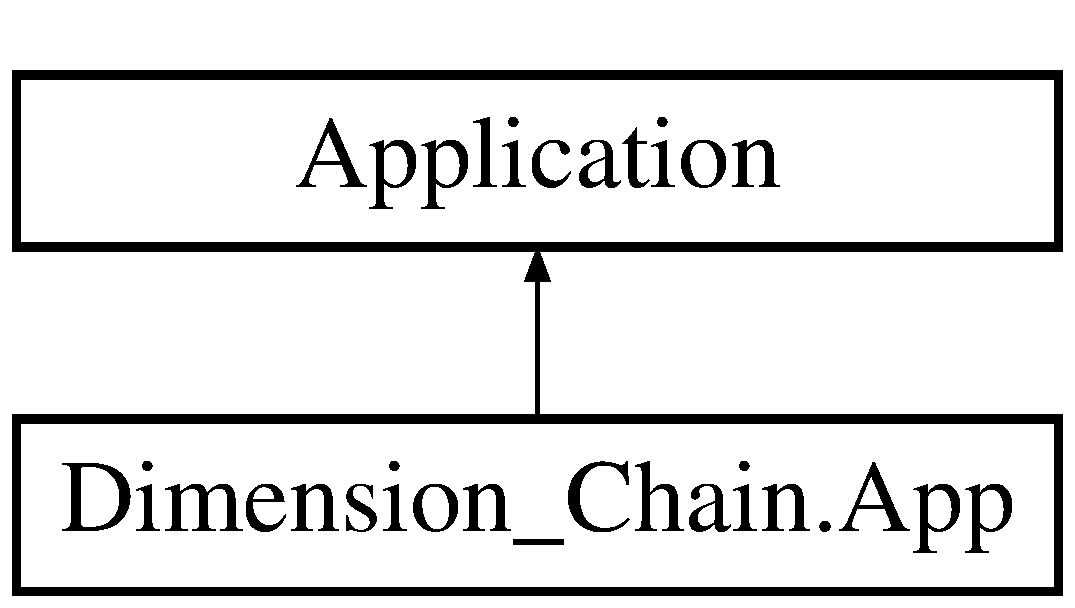
\includegraphics[height=2.000000cm]{class_dimension___chain_1_1_app}
\end{center}
\end{figure}


\subsection{Detailed Description}
Логика взаимодействия для App.\+xaml 



The documentation for this class was generated from the following file\+:\begin{DoxyCompactItemize}
\item 
\mbox{\hyperlink{_app_8xaml_8cs}{App.\+xaml.\+cs}}\end{DoxyCompactItemize}

\hypertarget{class_dimension___chain_1_1_constructor_user_control}{}\section{Dimension\+\_\+\+Chain.\+Constructor\+User\+Control Class Reference}
\label{class_dimension___chain_1_1_constructor_user_control}\index{Dimension\+\_\+\+Chain.\+Constructor\+User\+Control@{Dimension\+\_\+\+Chain.\+Constructor\+User\+Control}}


Логика взаимодействия для Constructor\+User\+Control.\+xaml  


Inheritance diagram for Dimension\+\_\+\+Chain.\+Constructor\+User\+Control\+:\begin{figure}[H]
\begin{center}
\leavevmode
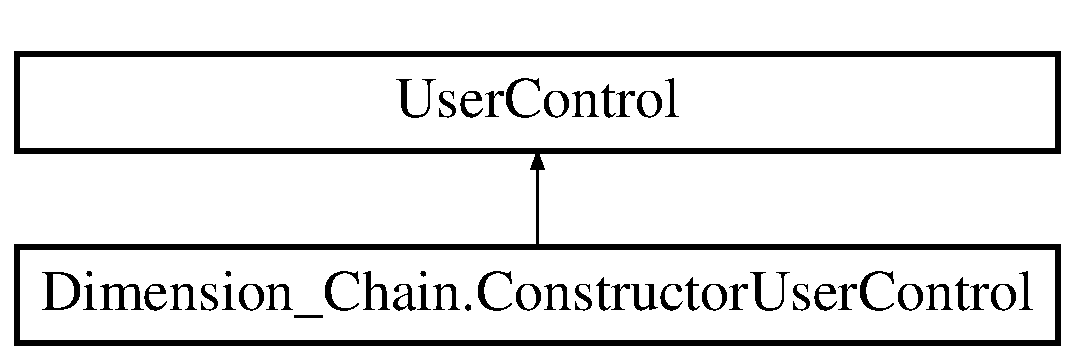
\includegraphics[height=2.000000cm]{class_dimension___chain_1_1_constructor_user_control}
\end{center}
\end{figure}
\subsection*{Public Member Functions}
\begin{DoxyCompactItemize}
\item 
\mbox{\hyperlink{class_dimension___chain_1_1_constructor_user_control_a2f3c1d13b26dcbe5a8e073c0c7ff6b37}{Constructor\+User\+Control}} ()
\item 
void \mbox{\hyperlink{class_dimension___chain_1_1_constructor_user_control_afef7cae9b0adc5fb1bfd6b5973c2fbc0}{Set\+U\+I\+\_\+\+CD}} (\mbox{\hyperlink{class_dimension___chain_1_1_u_i___constr_dimension}{U\+I\+\_\+\+Constr\+Dimension}} U\+I\+\_\+\+CD)
\item 
void \mbox{\hyperlink{class_dimension___chain_1_1_constructor_user_control_a4d13a15d714e5a5d84f3a9118daa42c7}{Re\+Null}} ()
\end{DoxyCompactItemize}


\subsection{Detailed Description}
Логика взаимодействия для Constructor\+User\+Control.\+xaml 



\subsection{Constructor \& Destructor Documentation}
\mbox{\Hypertarget{class_dimension___chain_1_1_constructor_user_control_a2f3c1d13b26dcbe5a8e073c0c7ff6b37}\label{class_dimension___chain_1_1_constructor_user_control_a2f3c1d13b26dcbe5a8e073c0c7ff6b37}} 
\index{Dimension\+\_\+\+Chain\+::\+Constructor\+User\+Control@{Dimension\+\_\+\+Chain\+::\+Constructor\+User\+Control}!Constructor\+User\+Control@{Constructor\+User\+Control}}
\index{Constructor\+User\+Control@{Constructor\+User\+Control}!Dimension\+\_\+\+Chain\+::\+Constructor\+User\+Control@{Dimension\+\_\+\+Chain\+::\+Constructor\+User\+Control}}
\subsubsection{\texorpdfstring{Constructor\+User\+Control()}{ConstructorUserControl()}}
{\footnotesize\ttfamily Dimension\+\_\+\+Chain.\+Constructor\+User\+Control.\+Constructor\+User\+Control (\begin{DoxyParamCaption}{ }\end{DoxyParamCaption})}



\subsection{Member Function Documentation}
\mbox{\Hypertarget{class_dimension___chain_1_1_constructor_user_control_a4d13a15d714e5a5d84f3a9118daa42c7}\label{class_dimension___chain_1_1_constructor_user_control_a4d13a15d714e5a5d84f3a9118daa42c7}} 
\index{Dimension\+\_\+\+Chain\+::\+Constructor\+User\+Control@{Dimension\+\_\+\+Chain\+::\+Constructor\+User\+Control}!Re\+Null@{Re\+Null}}
\index{Re\+Null@{Re\+Null}!Dimension\+\_\+\+Chain\+::\+Constructor\+User\+Control@{Dimension\+\_\+\+Chain\+::\+Constructor\+User\+Control}}
\subsubsection{\texorpdfstring{Re\+Null()}{ReNull()}}
{\footnotesize\ttfamily void Dimension\+\_\+\+Chain.\+Constructor\+User\+Control.\+Re\+Null (\begin{DoxyParamCaption}{ }\end{DoxyParamCaption})}

\mbox{\Hypertarget{class_dimension___chain_1_1_constructor_user_control_afef7cae9b0adc5fb1bfd6b5973c2fbc0}\label{class_dimension___chain_1_1_constructor_user_control_afef7cae9b0adc5fb1bfd6b5973c2fbc0}} 
\index{Dimension\+\_\+\+Chain\+::\+Constructor\+User\+Control@{Dimension\+\_\+\+Chain\+::\+Constructor\+User\+Control}!Set\+U\+I\+\_\+\+CD@{Set\+U\+I\+\_\+\+CD}}
\index{Set\+U\+I\+\_\+\+CD@{Set\+U\+I\+\_\+\+CD}!Dimension\+\_\+\+Chain\+::\+Constructor\+User\+Control@{Dimension\+\_\+\+Chain\+::\+Constructor\+User\+Control}}
\subsubsection{\texorpdfstring{Set\+U\+I\+\_\+\+C\+D()}{SetUI\_CD()}}
{\footnotesize\ttfamily void Dimension\+\_\+\+Chain.\+Constructor\+User\+Control.\+Set\+U\+I\+\_\+\+CD (\begin{DoxyParamCaption}\item[{\mbox{\hyperlink{class_dimension___chain_1_1_u_i___constr_dimension}{U\+I\+\_\+\+Constr\+Dimension}}}]{U\+I\+\_\+\+CD }\end{DoxyParamCaption})}



The documentation for this class was generated from the following file\+:\begin{DoxyCompactItemize}
\item 
\mbox{\hyperlink{_constructor_user_control_8xaml_8cs}{Constructor\+User\+Control.\+xaml.\+cs}}\end{DoxyCompactItemize}

\hypertarget{class_dimension___chain_1_1_controller}{}\section{Dimension\+\_\+\+Chain.\+Controller Class Reference}
\label{class_dimension___chain_1_1_controller}\index{Dimension\+\_\+\+Chain.\+Controller@{Dimension\+\_\+\+Chain.\+Controller}}
Inheritance diagram for Dimension\+\_\+\+Chain.\+Controller\+:\begin{figure}[H]
\begin{center}
\leavevmode
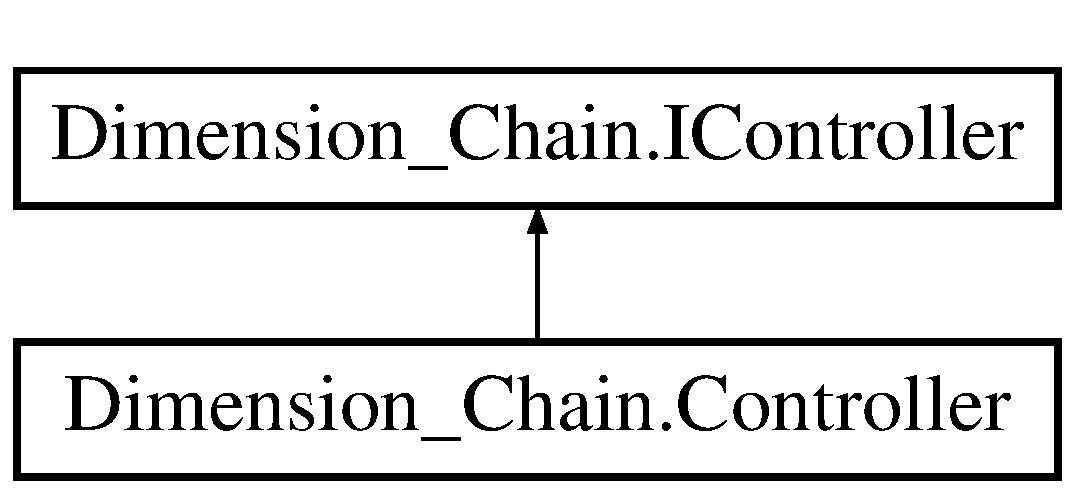
\includegraphics[height=2.000000cm]{class_dimension___chain_1_1_controller}
\end{center}
\end{figure}
\subsection*{Public Member Functions}
\begin{DoxyCompactItemize}
\item 
bool \mbox{\hyperlink{class_dimension___chain_1_1_controller_ae8c6a98ffe1507c958ca65e93d533c87}{is\+Create\+Dimension}} ()
\item 
\mbox{\hyperlink{class_dimension___chain_1_1_controller_a74201e6ac926c9d9028d0f465f037704}{Controller}} (Canvas canvas, Stack\+Panel left\+Stack\+Panel, Stack\+Panel right\+Stack\+Panel, \mbox{\hyperlink{class_dimension___chain_1_1_main_window}{Main\+Window}} window)
\item 
void \mbox{\hyperlink{class_dimension___chain_1_1_controller_a9e7eca33518de3a62888f2a6272cdeb6}{New\+Tech\+Dimension}} ()
\item 
void \mbox{\hyperlink{class_dimension___chain_1_1_controller_a5c809db2364ca8fd973b737cee2659b3}{New\+Prirusk}} ()
\begin{DoxyCompactList}\small\item\em Создание припуска \end{DoxyCompactList}\item 
void \mbox{\hyperlink{class_dimension___chain_1_1_controller_ac398246345f2b29698291b468aa0f491}{New\+Constr}} ()
\begin{DoxyCompactList}\small\item\em Создание конструкторского размера \end{DoxyCompactList}\end{DoxyCompactItemize}
\subsection*{Public Attributes}
\begin{DoxyCompactItemize}
\item 
\mbox{\hyperlink{class_dimension___chain_1_1_graph}{Graph}} \mbox{\hyperlink{class_dimension___chain_1_1_controller_ae84586e81da96ca1cc20a4044140769b}{graph}}
\item 
List$<$ \mbox{\hyperlink{class_dimension___chain_1_1_u_i___dimension}{U\+I\+\_\+\+Dimension}} $>$ \mbox{\hyperlink{class_dimension___chain_1_1_controller_acbb1b92f0d75262909a5d909afc99800}{list\+Of\+Dimensions}}
\end{DoxyCompactItemize}
\subsection*{Static Public Attributes}
\begin{DoxyCompactItemize}
\item 
static \mbox{\hyperlink{class_dimension___chain_1_1_tech_user_control}{Tech\+User\+Control}} \mbox{\hyperlink{class_dimension___chain_1_1_controller_a1547436a62102acbfce6b42eaabe4218}{T\+UC}} = new \mbox{\hyperlink{class_dimension___chain_1_1_tech_user_control}{Tech\+User\+Control}}()
\item 
static \mbox{\hyperlink{class_dimension___chain_1_1_pripusk_user_control}{Pripusk\+User\+Control}} \mbox{\hyperlink{class_dimension___chain_1_1_controller_a04aadf04988418c18ea1f1bb1f0fd59a}{P\+UC}} = new \mbox{\hyperlink{class_dimension___chain_1_1_pripusk_user_control}{Pripusk\+User\+Control}}()
\item 
static \mbox{\hyperlink{class_dimension___chain_1_1_constructor_user_control}{Constructor\+User\+Control}} \mbox{\hyperlink{class_dimension___chain_1_1_controller_a8541e9fa22540265ba3ca9bc0f8835da}{C\+UC}} = new \mbox{\hyperlink{class_dimension___chain_1_1_constructor_user_control}{Constructor\+User\+Control}}()
\end{DoxyCompactItemize}


\subsection{Constructor \& Destructor Documentation}
\mbox{\Hypertarget{class_dimension___chain_1_1_controller_a74201e6ac926c9d9028d0f465f037704}\label{class_dimension___chain_1_1_controller_a74201e6ac926c9d9028d0f465f037704}} 
\index{Dimension\+\_\+\+Chain\+::\+Controller@{Dimension\+\_\+\+Chain\+::\+Controller}!Controller@{Controller}}
\index{Controller@{Controller}!Dimension\+\_\+\+Chain\+::\+Controller@{Dimension\+\_\+\+Chain\+::\+Controller}}
\subsubsection{\texorpdfstring{Controller()}{Controller()}}
{\footnotesize\ttfamily Dimension\+\_\+\+Chain.\+Controller.\+Controller (\begin{DoxyParamCaption}\item[{Canvas}]{canvas,  }\item[{Stack\+Panel}]{left\+Stack\+Panel,  }\item[{Stack\+Panel}]{right\+Stack\+Panel,  }\item[{\mbox{\hyperlink{class_dimension___chain_1_1_main_window}{Main\+Window}}}]{window }\end{DoxyParamCaption})}



\subsection{Member Function Documentation}
\mbox{\Hypertarget{class_dimension___chain_1_1_controller_ae8c6a98ffe1507c958ca65e93d533c87}\label{class_dimension___chain_1_1_controller_ae8c6a98ffe1507c958ca65e93d533c87}} 
\index{Dimension\+\_\+\+Chain\+::\+Controller@{Dimension\+\_\+\+Chain\+::\+Controller}!is\+Create\+Dimension@{is\+Create\+Dimension}}
\index{is\+Create\+Dimension@{is\+Create\+Dimension}!Dimension\+\_\+\+Chain\+::\+Controller@{Dimension\+\_\+\+Chain\+::\+Controller}}
\subsubsection{\texorpdfstring{is\+Create\+Dimension()}{isCreateDimension()}}
{\footnotesize\ttfamily bool Dimension\+\_\+\+Chain.\+Controller.\+is\+Create\+Dimension (\begin{DoxyParamCaption}{ }\end{DoxyParamCaption})}



Implements \mbox{\hyperlink{interface_dimension___chain_1_1_i_controller_a228ee16ef616fee00fc5141e3ebef9db}{Dimension\+\_\+\+Chain.\+I\+Controller}}.

\mbox{\Hypertarget{class_dimension___chain_1_1_controller_ac398246345f2b29698291b468aa0f491}\label{class_dimension___chain_1_1_controller_ac398246345f2b29698291b468aa0f491}} 
\index{Dimension\+\_\+\+Chain\+::\+Controller@{Dimension\+\_\+\+Chain\+::\+Controller}!New\+Constr@{New\+Constr}}
\index{New\+Constr@{New\+Constr}!Dimension\+\_\+\+Chain\+::\+Controller@{Dimension\+\_\+\+Chain\+::\+Controller}}
\subsubsection{\texorpdfstring{New\+Constr()}{NewConstr()}}
{\footnotesize\ttfamily void Dimension\+\_\+\+Chain.\+Controller.\+New\+Constr (\begin{DoxyParamCaption}{ }\end{DoxyParamCaption})}



Создание конструкторского размера 

\mbox{\Hypertarget{class_dimension___chain_1_1_controller_a5c809db2364ca8fd973b737cee2659b3}\label{class_dimension___chain_1_1_controller_a5c809db2364ca8fd973b737cee2659b3}} 
\index{Dimension\+\_\+\+Chain\+::\+Controller@{Dimension\+\_\+\+Chain\+::\+Controller}!New\+Prirusk@{New\+Prirusk}}
\index{New\+Prirusk@{New\+Prirusk}!Dimension\+\_\+\+Chain\+::\+Controller@{Dimension\+\_\+\+Chain\+::\+Controller}}
\subsubsection{\texorpdfstring{New\+Prirusk()}{NewPrirusk()}}
{\footnotesize\ttfamily void Dimension\+\_\+\+Chain.\+Controller.\+New\+Prirusk (\begin{DoxyParamCaption}{ }\end{DoxyParamCaption})}



Создание припуска 

\mbox{\Hypertarget{class_dimension___chain_1_1_controller_a9e7eca33518de3a62888f2a6272cdeb6}\label{class_dimension___chain_1_1_controller_a9e7eca33518de3a62888f2a6272cdeb6}} 
\index{Dimension\+\_\+\+Chain\+::\+Controller@{Dimension\+\_\+\+Chain\+::\+Controller}!New\+Tech\+Dimension@{New\+Tech\+Dimension}}
\index{New\+Tech\+Dimension@{New\+Tech\+Dimension}!Dimension\+\_\+\+Chain\+::\+Controller@{Dimension\+\_\+\+Chain\+::\+Controller}}
\subsubsection{\texorpdfstring{New\+Tech\+Dimension()}{NewTechDimension()}}
{\footnotesize\ttfamily void Dimension\+\_\+\+Chain.\+Controller.\+New\+Tech\+Dimension (\begin{DoxyParamCaption}{ }\end{DoxyParamCaption})}





Создание технологического размера 

\subsection{Member Data Documentation}
\mbox{\Hypertarget{class_dimension___chain_1_1_controller_a8541e9fa22540265ba3ca9bc0f8835da}\label{class_dimension___chain_1_1_controller_a8541e9fa22540265ba3ca9bc0f8835da}} 
\index{Dimension\+\_\+\+Chain\+::\+Controller@{Dimension\+\_\+\+Chain\+::\+Controller}!C\+UC@{C\+UC}}
\index{C\+UC@{C\+UC}!Dimension\+\_\+\+Chain\+::\+Controller@{Dimension\+\_\+\+Chain\+::\+Controller}}
\subsubsection{\texorpdfstring{C\+UC}{CUC}}
{\footnotesize\ttfamily \mbox{\hyperlink{class_dimension___chain_1_1_constructor_user_control}{Constructor\+User\+Control}} Dimension\+\_\+\+Chain.\+Controller.\+C\+UC = new \mbox{\hyperlink{class_dimension___chain_1_1_constructor_user_control}{Constructor\+User\+Control}}()\hspace{0.3cm}{\ttfamily [static]}}

\mbox{\Hypertarget{class_dimension___chain_1_1_controller_ae84586e81da96ca1cc20a4044140769b}\label{class_dimension___chain_1_1_controller_ae84586e81da96ca1cc20a4044140769b}} 
\index{Dimension\+\_\+\+Chain\+::\+Controller@{Dimension\+\_\+\+Chain\+::\+Controller}!graph@{graph}}
\index{graph@{graph}!Dimension\+\_\+\+Chain\+::\+Controller@{Dimension\+\_\+\+Chain\+::\+Controller}}
\subsubsection{\texorpdfstring{graph}{graph}}
{\footnotesize\ttfamily \mbox{\hyperlink{class_dimension___chain_1_1_graph}{Graph}} Dimension\+\_\+\+Chain.\+Controller.\+graph}

\mbox{\Hypertarget{class_dimension___chain_1_1_controller_acbb1b92f0d75262909a5d909afc99800}\label{class_dimension___chain_1_1_controller_acbb1b92f0d75262909a5d909afc99800}} 
\index{Dimension\+\_\+\+Chain\+::\+Controller@{Dimension\+\_\+\+Chain\+::\+Controller}!list\+Of\+Dimensions@{list\+Of\+Dimensions}}
\index{list\+Of\+Dimensions@{list\+Of\+Dimensions}!Dimension\+\_\+\+Chain\+::\+Controller@{Dimension\+\_\+\+Chain\+::\+Controller}}
\subsubsection{\texorpdfstring{list\+Of\+Dimensions}{listOfDimensions}}
{\footnotesize\ttfamily List$<$\mbox{\hyperlink{class_dimension___chain_1_1_u_i___dimension}{U\+I\+\_\+\+Dimension}}$>$ Dimension\+\_\+\+Chain.\+Controller.\+list\+Of\+Dimensions}

\mbox{\Hypertarget{class_dimension___chain_1_1_controller_a04aadf04988418c18ea1f1bb1f0fd59a}\label{class_dimension___chain_1_1_controller_a04aadf04988418c18ea1f1bb1f0fd59a}} 
\index{Dimension\+\_\+\+Chain\+::\+Controller@{Dimension\+\_\+\+Chain\+::\+Controller}!P\+UC@{P\+UC}}
\index{P\+UC@{P\+UC}!Dimension\+\_\+\+Chain\+::\+Controller@{Dimension\+\_\+\+Chain\+::\+Controller}}
\subsubsection{\texorpdfstring{P\+UC}{PUC}}
{\footnotesize\ttfamily \mbox{\hyperlink{class_dimension___chain_1_1_pripusk_user_control}{Pripusk\+User\+Control}} Dimension\+\_\+\+Chain.\+Controller.\+P\+UC = new \mbox{\hyperlink{class_dimension___chain_1_1_pripusk_user_control}{Pripusk\+User\+Control}}()\hspace{0.3cm}{\ttfamily [static]}}

\mbox{\Hypertarget{class_dimension___chain_1_1_controller_a1547436a62102acbfce6b42eaabe4218}\label{class_dimension___chain_1_1_controller_a1547436a62102acbfce6b42eaabe4218}} 
\index{Dimension\+\_\+\+Chain\+::\+Controller@{Dimension\+\_\+\+Chain\+::\+Controller}!T\+UC@{T\+UC}}
\index{T\+UC@{T\+UC}!Dimension\+\_\+\+Chain\+::\+Controller@{Dimension\+\_\+\+Chain\+::\+Controller}}
\subsubsection{\texorpdfstring{T\+UC}{TUC}}
{\footnotesize\ttfamily \mbox{\hyperlink{class_dimension___chain_1_1_tech_user_control}{Tech\+User\+Control}} Dimension\+\_\+\+Chain.\+Controller.\+T\+UC = new \mbox{\hyperlink{class_dimension___chain_1_1_tech_user_control}{Tech\+User\+Control}}()\hspace{0.3cm}{\ttfamily [static]}}



The documentation for this class was generated from the following file\+:\begin{DoxyCompactItemize}
\item 
\mbox{\hyperlink{_controller_8cs}{Controller.\+cs}}\end{DoxyCompactItemize}

\hypertarget{class_dimension___chain_1_1_dimension}{}\section{Dimension\+\_\+\+Chain.\+Dimension Class Reference}
\label{class_dimension___chain_1_1_dimension}\index{Dimension\+\_\+\+Chain.\+Dimension@{Dimension\+\_\+\+Chain.\+Dimension}}
\subsection*{Public Member Functions}
\begin{DoxyCompactItemize}
\item 
\mbox{\hyperlink{class_dimension___chain_1_1_dimension_a4d20f1328ddc226bcbdf693ab62782d2}{Dimension}} (\mbox{\hyperlink{class_dimension___chain_1_1_vertex}{Vertex}} \mbox{\hyperlink{class_dimension___chain_1_1_dimension_a2eba65a35b73d444960c5b7640f3a44a}{first\+Vertex}}, \mbox{\hyperlink{class_dimension___chain_1_1_vertex}{Vertex}} \mbox{\hyperlink{class_dimension___chain_1_1_dimension_af58340b2d25b2de18c1fc796ad5aedeb}{second\+Vertex}}, \mbox{\hyperlink{namespace_dimension___chain_a6ec9051138598c61cc00acf2547dced4}{type}} \mbox{\hyperlink{class_dimension___chain_1_1_dimension_ac18f5f8b3700a2ce95008310acf6213f}{\+\_\+type}}, \mbox{\hyperlink{class_dimension___chain_1_1_value}{Value}} \mbox{\hyperlink{class_dimension___chain_1_1_dimension_a742090c0440d5a7474adf61c071f5e47}{value}})
\end{DoxyCompactItemize}
\subsection*{Public Attributes}
\begin{DoxyCompactItemize}
\item 
\mbox{\hyperlink{class_dimension___chain_1_1_vertex}{Vertex}} \mbox{\hyperlink{class_dimension___chain_1_1_dimension_a2eba65a35b73d444960c5b7640f3a44a}{first\+Vertex}}
\item 
\mbox{\hyperlink{class_dimension___chain_1_1_vertex}{Vertex}} \mbox{\hyperlink{class_dimension___chain_1_1_dimension_af58340b2d25b2de18c1fc796ad5aedeb}{second\+Vertex}}
\item 
\mbox{\hyperlink{namespace_dimension___chain_a6ec9051138598c61cc00acf2547dced4}{type}} \mbox{\hyperlink{class_dimension___chain_1_1_dimension_ac18f5f8b3700a2ce95008310acf6213f}{\+\_\+type}}
\item 
\mbox{\hyperlink{class_dimension___chain_1_1_value}{Value}} \mbox{\hyperlink{class_dimension___chain_1_1_dimension_a742090c0440d5a7474adf61c071f5e47}{value}}
\item 
bool \mbox{\hyperlink{class_dimension___chain_1_1_dimension_ab0492cdbb367b933ad455eacfd2e9c71}{visited}}
\end{DoxyCompactItemize}


\subsection{Constructor \& Destructor Documentation}
\mbox{\Hypertarget{class_dimension___chain_1_1_dimension_a4d20f1328ddc226bcbdf693ab62782d2}\label{class_dimension___chain_1_1_dimension_a4d20f1328ddc226bcbdf693ab62782d2}} 
\index{Dimension\+\_\+\+Chain\+::\+Dimension@{Dimension\+\_\+\+Chain\+::\+Dimension}!Dimension@{Dimension}}
\index{Dimension@{Dimension}!Dimension\+\_\+\+Chain\+::\+Dimension@{Dimension\+\_\+\+Chain\+::\+Dimension}}
\subsubsection{\texorpdfstring{Dimension()}{Dimension()}}
{\footnotesize\ttfamily Dimension\+\_\+\+Chain.\+Dimension.\+Dimension (\begin{DoxyParamCaption}\item[{\mbox{\hyperlink{class_dimension___chain_1_1_vertex}{Vertex}}}]{first\+Vertex,  }\item[{\mbox{\hyperlink{class_dimension___chain_1_1_vertex}{Vertex}}}]{second\+Vertex,  }\item[{\mbox{\hyperlink{namespace_dimension___chain_a6ec9051138598c61cc00acf2547dced4}{type}}}]{\+\_\+type,  }\item[{\mbox{\hyperlink{class_dimension___chain_1_1_value}{Value}}}]{value }\end{DoxyParamCaption})}



\subsection{Member Data Documentation}
\mbox{\Hypertarget{class_dimension___chain_1_1_dimension_ac18f5f8b3700a2ce95008310acf6213f}\label{class_dimension___chain_1_1_dimension_ac18f5f8b3700a2ce95008310acf6213f}} 
\index{Dimension\+\_\+\+Chain\+::\+Dimension@{Dimension\+\_\+\+Chain\+::\+Dimension}!\+\_\+type@{\+\_\+type}}
\index{\+\_\+type@{\+\_\+type}!Dimension\+\_\+\+Chain\+::\+Dimension@{Dimension\+\_\+\+Chain\+::\+Dimension}}
\subsubsection{\texorpdfstring{\+\_\+type}{\_type}}
{\footnotesize\ttfamily \mbox{\hyperlink{namespace_dimension___chain_a6ec9051138598c61cc00acf2547dced4}{type}} Dimension\+\_\+\+Chain.\+Dimension.\+\_\+type}

\mbox{\Hypertarget{class_dimension___chain_1_1_dimension_a2eba65a35b73d444960c5b7640f3a44a}\label{class_dimension___chain_1_1_dimension_a2eba65a35b73d444960c5b7640f3a44a}} 
\index{Dimension\+\_\+\+Chain\+::\+Dimension@{Dimension\+\_\+\+Chain\+::\+Dimension}!first\+Vertex@{first\+Vertex}}
\index{first\+Vertex@{first\+Vertex}!Dimension\+\_\+\+Chain\+::\+Dimension@{Dimension\+\_\+\+Chain\+::\+Dimension}}
\subsubsection{\texorpdfstring{first\+Vertex}{firstVertex}}
{\footnotesize\ttfamily \mbox{\hyperlink{class_dimension___chain_1_1_vertex}{Vertex}} Dimension\+\_\+\+Chain.\+Dimension.\+first\+Vertex}

\mbox{\Hypertarget{class_dimension___chain_1_1_dimension_af58340b2d25b2de18c1fc796ad5aedeb}\label{class_dimension___chain_1_1_dimension_af58340b2d25b2de18c1fc796ad5aedeb}} 
\index{Dimension\+\_\+\+Chain\+::\+Dimension@{Dimension\+\_\+\+Chain\+::\+Dimension}!second\+Vertex@{second\+Vertex}}
\index{second\+Vertex@{second\+Vertex}!Dimension\+\_\+\+Chain\+::\+Dimension@{Dimension\+\_\+\+Chain\+::\+Dimension}}
\subsubsection{\texorpdfstring{second\+Vertex}{secondVertex}}
{\footnotesize\ttfamily \mbox{\hyperlink{class_dimension___chain_1_1_vertex}{Vertex}} Dimension\+\_\+\+Chain.\+Dimension.\+second\+Vertex}

\mbox{\Hypertarget{class_dimension___chain_1_1_dimension_a742090c0440d5a7474adf61c071f5e47}\label{class_dimension___chain_1_1_dimension_a742090c0440d5a7474adf61c071f5e47}} 
\index{Dimension\+\_\+\+Chain\+::\+Dimension@{Dimension\+\_\+\+Chain\+::\+Dimension}!value@{value}}
\index{value@{value}!Dimension\+\_\+\+Chain\+::\+Dimension@{Dimension\+\_\+\+Chain\+::\+Dimension}}
\subsubsection{\texorpdfstring{value}{value}}
{\footnotesize\ttfamily \mbox{\hyperlink{class_dimension___chain_1_1_value}{Value}} Dimension\+\_\+\+Chain.\+Dimension.\+value}

\mbox{\Hypertarget{class_dimension___chain_1_1_dimension_ab0492cdbb367b933ad455eacfd2e9c71}\label{class_dimension___chain_1_1_dimension_ab0492cdbb367b933ad455eacfd2e9c71}} 
\index{Dimension\+\_\+\+Chain\+::\+Dimension@{Dimension\+\_\+\+Chain\+::\+Dimension}!visited@{visited}}
\index{visited@{visited}!Dimension\+\_\+\+Chain\+::\+Dimension@{Dimension\+\_\+\+Chain\+::\+Dimension}}
\subsubsection{\texorpdfstring{visited}{visited}}
{\footnotesize\ttfamily bool Dimension\+\_\+\+Chain.\+Dimension.\+visited}



The documentation for this class was generated from the following file\+:\begin{DoxyCompactItemize}
\item 
\mbox{\hyperlink{_dimension_8cs}{Dimension.\+cs}}\end{DoxyCompactItemize}

\hypertarget{class_dimension___chain_1_1_graph}{}\section{Dimension\+\_\+\+Chain.\+Graph Class Reference}
\label{class_dimension___chain_1_1_graph}\index{Dimension\+\_\+\+Chain.\+Graph@{Dimension\+\_\+\+Chain.\+Graph}}
\subsection*{Public Member Functions}
\begin{DoxyCompactItemize}
\item 
\mbox{\hyperlink{class_dimension___chain_1_1_vertex}{Vertex}} \mbox{\hyperlink{class_dimension___chain_1_1_graph_ac175fc4299e2577a99d7b6c197bae4d2}{Create\+Vertex}} ()
\item 
bool \mbox{\hyperlink{class_dimension___chain_1_1_graph_a7b424d53464cbb322db7944f2ad6bb7a}{Create\+Nul}} (\mbox{\hyperlink{class_dimension___chain_1_1_vertex}{Vertex}} v1, \mbox{\hyperlink{class_dimension___chain_1_1_vertex}{Vertex}} v2)
\item 
\mbox{\hyperlink{class_dimension___chain_1_1_dimension}{Dimension}} \mbox{\hyperlink{class_dimension___chain_1_1_graph_ada5a731ebbb09267d501292d27db32fc}{Create\+Closing\+Link}} (\mbox{\hyperlink{class_dimension___chain_1_1_vertex}{Vertex}} v1, \mbox{\hyperlink{class_dimension___chain_1_1_vertex}{Vertex}} v2, \mbox{\hyperlink{namespace_dimension___chain_a6ec9051138598c61cc00acf2547dced4}{type}} typ)
\item 
\mbox{\hyperlink{class_dimension___chain_1_1_dimension}{Dimension}} \mbox{\hyperlink{class_dimension___chain_1_1_graph_a2a5db4af48b7b6c7595a79912b47c81e}{Create\+Tech\+Dimension}} (\mbox{\hyperlink{class_dimension___chain_1_1_vertex}{Vertex}} v1, \mbox{\hyperlink{class_dimension___chain_1_1_vertex}{Vertex}} v2, \mbox{\hyperlink{class_dimension___chain_1_1_value}{Value}} val)
\item 
void \mbox{\hyperlink{class_dimension___chain_1_1_graph_a781ea9fd0f61ebf19698b1964b7a9f15}{Delete\+Dimension}} (\mbox{\hyperlink{class_dimension___chain_1_1_dimension}{Dimension}} dim)
\begin{DoxyCompactList}\small\item\em Удаление размера и всех связанных с ним вершин и всех связанных с ними размерами \end{DoxyCompactList}\item 
\mbox{\hyperlink{class_dimension___chain_1_1_value}{Value}} \mbox{\hyperlink{class_dimension___chain_1_1_graph_a3817dc05a66fc09a8655ac35a63434a2}{B\+F\+S\+\_\+\+Find\+Short\+Way}} (\mbox{\hyperlink{class_dimension___chain_1_1_vertex}{Vertex}} source, \mbox{\hyperlink{class_dimension___chain_1_1_vertex}{Vertex}} destination, List$<$ \mbox{\hyperlink{class_dimension___chain_1_1_dimension}{Dimension}} $>$ received\+List)
\item 
void \mbox{\hyperlink{class_dimension___chain_1_1_graph_af94dc71f4cffd52f1eba00301d9e450b}{Visited\+False}} ()
\end{DoxyCompactItemize}
\subsection*{Public Attributes}
\begin{DoxyCompactItemize}
\item 
int \mbox{\hyperlink{class_dimension___chain_1_1_graph_a787a940fcdc7c2a3e65a53762b983d4f}{num}} = 0
\item 
List$<$ \mbox{\hyperlink{class_dimension___chain_1_1_vertex}{Vertex}} $>$ \mbox{\hyperlink{class_dimension___chain_1_1_graph_a74a6519101a76d81f7ad02c72915648a}{vertex\+List}} = new List$<$\mbox{\hyperlink{class_dimension___chain_1_1_vertex}{Vertex}}$>$()
\item 
List$<$ \mbox{\hyperlink{class_dimension___chain_1_1_dimension}{Dimension}} $>$ \mbox{\hyperlink{class_dimension___chain_1_1_graph_a97809fd98170fabe659b9de4c9202605}{dimension\+List}} = new List$<$\mbox{\hyperlink{class_dimension___chain_1_1_dimension}{Dimension}}$>$()
\end{DoxyCompactItemize}
\subsection*{Properties}
\begin{DoxyCompactItemize}
\item 
bool \mbox{\hyperlink{class_dimension___chain_1_1_graph_a3b83aa20522a80c1e33ee1975a705278}{is\+Cicle}}\hspace{0.3cm}{\ttfamily  \mbox{[}get\mbox{]}}
\end{DoxyCompactItemize}


\subsection{Member Function Documentation}
\mbox{\Hypertarget{class_dimension___chain_1_1_graph_a3817dc05a66fc09a8655ac35a63434a2}\label{class_dimension___chain_1_1_graph_a3817dc05a66fc09a8655ac35a63434a2}} 
\index{Dimension\+\_\+\+Chain\+::\+Graph@{Dimension\+\_\+\+Chain\+::\+Graph}!B\+F\+S\+\_\+\+Find\+Short\+Way@{B\+F\+S\+\_\+\+Find\+Short\+Way}}
\index{B\+F\+S\+\_\+\+Find\+Short\+Way@{B\+F\+S\+\_\+\+Find\+Short\+Way}!Dimension\+\_\+\+Chain\+::\+Graph@{Dimension\+\_\+\+Chain\+::\+Graph}}
\subsubsection{\texorpdfstring{B\+F\+S\+\_\+\+Find\+Short\+Way()}{BFS\_FindShortWay()}}
{\footnotesize\ttfamily \mbox{\hyperlink{class_dimension___chain_1_1_value}{Value}} Dimension\+\_\+\+Chain.\+Graph.\+B\+F\+S\+\_\+\+Find\+Short\+Way (\begin{DoxyParamCaption}\item[{\mbox{\hyperlink{class_dimension___chain_1_1_vertex}{Vertex}}}]{source,  }\item[{\mbox{\hyperlink{class_dimension___chain_1_1_vertex}{Vertex}}}]{destination,  }\item[{List$<$ \mbox{\hyperlink{class_dimension___chain_1_1_dimension}{Dimension}} $>$}]{received\+List }\end{DoxyParamCaption})}

\mbox{\Hypertarget{class_dimension___chain_1_1_graph_ada5a731ebbb09267d501292d27db32fc}\label{class_dimension___chain_1_1_graph_ada5a731ebbb09267d501292d27db32fc}} 
\index{Dimension\+\_\+\+Chain\+::\+Graph@{Dimension\+\_\+\+Chain\+::\+Graph}!Create\+Closing\+Link@{Create\+Closing\+Link}}
\index{Create\+Closing\+Link@{Create\+Closing\+Link}!Dimension\+\_\+\+Chain\+::\+Graph@{Dimension\+\_\+\+Chain\+::\+Graph}}
\subsubsection{\texorpdfstring{Create\+Closing\+Link()}{CreateClosingLink()}}
{\footnotesize\ttfamily \mbox{\hyperlink{class_dimension___chain_1_1_dimension}{Dimension}} Dimension\+\_\+\+Chain.\+Graph.\+Create\+Closing\+Link (\begin{DoxyParamCaption}\item[{\mbox{\hyperlink{class_dimension___chain_1_1_vertex}{Vertex}}}]{v1,  }\item[{\mbox{\hyperlink{class_dimension___chain_1_1_vertex}{Vertex}}}]{v2,  }\item[{\mbox{\hyperlink{namespace_dimension___chain_a6ec9051138598c61cc00acf2547dced4}{type}}}]{typ }\end{DoxyParamCaption})}

\mbox{\Hypertarget{class_dimension___chain_1_1_graph_a7b424d53464cbb322db7944f2ad6bb7a}\label{class_dimension___chain_1_1_graph_a7b424d53464cbb322db7944f2ad6bb7a}} 
\index{Dimension\+\_\+\+Chain\+::\+Graph@{Dimension\+\_\+\+Chain\+::\+Graph}!Create\+Nul@{Create\+Nul}}
\index{Create\+Nul@{Create\+Nul}!Dimension\+\_\+\+Chain\+::\+Graph@{Dimension\+\_\+\+Chain\+::\+Graph}}
\subsubsection{\texorpdfstring{Create\+Nul()}{CreateNul()}}
{\footnotesize\ttfamily bool Dimension\+\_\+\+Chain.\+Graph.\+Create\+Nul (\begin{DoxyParamCaption}\item[{\mbox{\hyperlink{class_dimension___chain_1_1_vertex}{Vertex}}}]{v1,  }\item[{\mbox{\hyperlink{class_dimension___chain_1_1_vertex}{Vertex}}}]{v2 }\end{DoxyParamCaption})}

\mbox{\Hypertarget{class_dimension___chain_1_1_graph_a2a5db4af48b7b6c7595a79912b47c81e}\label{class_dimension___chain_1_1_graph_a2a5db4af48b7b6c7595a79912b47c81e}} 
\index{Dimension\+\_\+\+Chain\+::\+Graph@{Dimension\+\_\+\+Chain\+::\+Graph}!Create\+Tech\+Dimension@{Create\+Tech\+Dimension}}
\index{Create\+Tech\+Dimension@{Create\+Tech\+Dimension}!Dimension\+\_\+\+Chain\+::\+Graph@{Dimension\+\_\+\+Chain\+::\+Graph}}
\subsubsection{\texorpdfstring{Create\+Tech\+Dimension()}{CreateTechDimension()}}
{\footnotesize\ttfamily \mbox{\hyperlink{class_dimension___chain_1_1_dimension}{Dimension}} Dimension\+\_\+\+Chain.\+Graph.\+Create\+Tech\+Dimension (\begin{DoxyParamCaption}\item[{\mbox{\hyperlink{class_dimension___chain_1_1_vertex}{Vertex}}}]{v1,  }\item[{\mbox{\hyperlink{class_dimension___chain_1_1_vertex}{Vertex}}}]{v2,  }\item[{\mbox{\hyperlink{class_dimension___chain_1_1_value}{Value}}}]{val }\end{DoxyParamCaption})}

\mbox{\Hypertarget{class_dimension___chain_1_1_graph_ac175fc4299e2577a99d7b6c197bae4d2}\label{class_dimension___chain_1_1_graph_ac175fc4299e2577a99d7b6c197bae4d2}} 
\index{Dimension\+\_\+\+Chain\+::\+Graph@{Dimension\+\_\+\+Chain\+::\+Graph}!Create\+Vertex@{Create\+Vertex}}
\index{Create\+Vertex@{Create\+Vertex}!Dimension\+\_\+\+Chain\+::\+Graph@{Dimension\+\_\+\+Chain\+::\+Graph}}
\subsubsection{\texorpdfstring{Create\+Vertex()}{CreateVertex()}}
{\footnotesize\ttfamily \mbox{\hyperlink{class_dimension___chain_1_1_vertex}{Vertex}} Dimension\+\_\+\+Chain.\+Graph.\+Create\+Vertex (\begin{DoxyParamCaption}{ }\end{DoxyParamCaption})}

\mbox{\Hypertarget{class_dimension___chain_1_1_graph_a781ea9fd0f61ebf19698b1964b7a9f15}\label{class_dimension___chain_1_1_graph_a781ea9fd0f61ebf19698b1964b7a9f15}} 
\index{Dimension\+\_\+\+Chain\+::\+Graph@{Dimension\+\_\+\+Chain\+::\+Graph}!Delete\+Dimension@{Delete\+Dimension}}
\index{Delete\+Dimension@{Delete\+Dimension}!Dimension\+\_\+\+Chain\+::\+Graph@{Dimension\+\_\+\+Chain\+::\+Graph}}
\subsubsection{\texorpdfstring{Delete\+Dimension()}{DeleteDimension()}}
{\footnotesize\ttfamily void Dimension\+\_\+\+Chain.\+Graph.\+Delete\+Dimension (\begin{DoxyParamCaption}\item[{\mbox{\hyperlink{class_dimension___chain_1_1_dimension}{Dimension}}}]{dim }\end{DoxyParamCaption})}



Удаление размера и всех связанных с ним вершин и всех связанных с ними размерами 


\begin{DoxyParams}{Parameters}
{\em dim} & Удаляемый размер\\
\hline
\end{DoxyParams}
\mbox{\Hypertarget{class_dimension___chain_1_1_graph_af94dc71f4cffd52f1eba00301d9e450b}\label{class_dimension___chain_1_1_graph_af94dc71f4cffd52f1eba00301d9e450b}} 
\index{Dimension\+\_\+\+Chain\+::\+Graph@{Dimension\+\_\+\+Chain\+::\+Graph}!Visited\+False@{Visited\+False}}
\index{Visited\+False@{Visited\+False}!Dimension\+\_\+\+Chain\+::\+Graph@{Dimension\+\_\+\+Chain\+::\+Graph}}
\subsubsection{\texorpdfstring{Visited\+False()}{VisitedFalse()}}
{\footnotesize\ttfamily void Dimension\+\_\+\+Chain.\+Graph.\+Visited\+False (\begin{DoxyParamCaption}{ }\end{DoxyParamCaption})}



\subsection{Member Data Documentation}
\mbox{\Hypertarget{class_dimension___chain_1_1_graph_a97809fd98170fabe659b9de4c9202605}\label{class_dimension___chain_1_1_graph_a97809fd98170fabe659b9de4c9202605}} 
\index{Dimension\+\_\+\+Chain\+::\+Graph@{Dimension\+\_\+\+Chain\+::\+Graph}!dimension\+List@{dimension\+List}}
\index{dimension\+List@{dimension\+List}!Dimension\+\_\+\+Chain\+::\+Graph@{Dimension\+\_\+\+Chain\+::\+Graph}}
\subsubsection{\texorpdfstring{dimension\+List}{dimensionList}}
{\footnotesize\ttfamily List$<$\mbox{\hyperlink{class_dimension___chain_1_1_dimension}{Dimension}}$>$ Dimension\+\_\+\+Chain.\+Graph.\+dimension\+List = new List$<$\mbox{\hyperlink{class_dimension___chain_1_1_dimension}{Dimension}}$>$()}

\mbox{\Hypertarget{class_dimension___chain_1_1_graph_a787a940fcdc7c2a3e65a53762b983d4f}\label{class_dimension___chain_1_1_graph_a787a940fcdc7c2a3e65a53762b983d4f}} 
\index{Dimension\+\_\+\+Chain\+::\+Graph@{Dimension\+\_\+\+Chain\+::\+Graph}!num@{num}}
\index{num@{num}!Dimension\+\_\+\+Chain\+::\+Graph@{Dimension\+\_\+\+Chain\+::\+Graph}}
\subsubsection{\texorpdfstring{num}{num}}
{\footnotesize\ttfamily int Dimension\+\_\+\+Chain.\+Graph.\+num = 0}

\mbox{\Hypertarget{class_dimension___chain_1_1_graph_a74a6519101a76d81f7ad02c72915648a}\label{class_dimension___chain_1_1_graph_a74a6519101a76d81f7ad02c72915648a}} 
\index{Dimension\+\_\+\+Chain\+::\+Graph@{Dimension\+\_\+\+Chain\+::\+Graph}!vertex\+List@{vertex\+List}}
\index{vertex\+List@{vertex\+List}!Dimension\+\_\+\+Chain\+::\+Graph@{Dimension\+\_\+\+Chain\+::\+Graph}}
\subsubsection{\texorpdfstring{vertex\+List}{vertexList}}
{\footnotesize\ttfamily List$<$\mbox{\hyperlink{class_dimension___chain_1_1_vertex}{Vertex}}$>$ Dimension\+\_\+\+Chain.\+Graph.\+vertex\+List = new List$<$\mbox{\hyperlink{class_dimension___chain_1_1_vertex}{Vertex}}$>$()}



\subsection{Property Documentation}
\mbox{\Hypertarget{class_dimension___chain_1_1_graph_a3b83aa20522a80c1e33ee1975a705278}\label{class_dimension___chain_1_1_graph_a3b83aa20522a80c1e33ee1975a705278}} 
\index{Dimension\+\_\+\+Chain\+::\+Graph@{Dimension\+\_\+\+Chain\+::\+Graph}!is\+Cicle@{is\+Cicle}}
\index{is\+Cicle@{is\+Cicle}!Dimension\+\_\+\+Chain\+::\+Graph@{Dimension\+\_\+\+Chain\+::\+Graph}}
\subsubsection{\texorpdfstring{is\+Cicle}{isCicle}}
{\footnotesize\ttfamily bool Dimension\+\_\+\+Chain.\+Graph.\+is\+Cicle\hspace{0.3cm}{\ttfamily [get]}}



The documentation for this class was generated from the following file\+:\begin{DoxyCompactItemize}
\item 
\mbox{\hyperlink{_graph_8cs}{Graph.\+cs}}\end{DoxyCompactItemize}

\hypertarget{interface_dimension___chain_1_1_i_controller}{}\section{Dimension\+\_\+\+Chain.\+I\+Controller Interface Reference}
\label{interface_dimension___chain_1_1_i_controller}\index{Dimension\+\_\+\+Chain.\+I\+Controller@{Dimension\+\_\+\+Chain.\+I\+Controller}}
Inheritance diagram for Dimension\+\_\+\+Chain.\+I\+Controller\+:\begin{figure}[H]
\begin{center}
\leavevmode
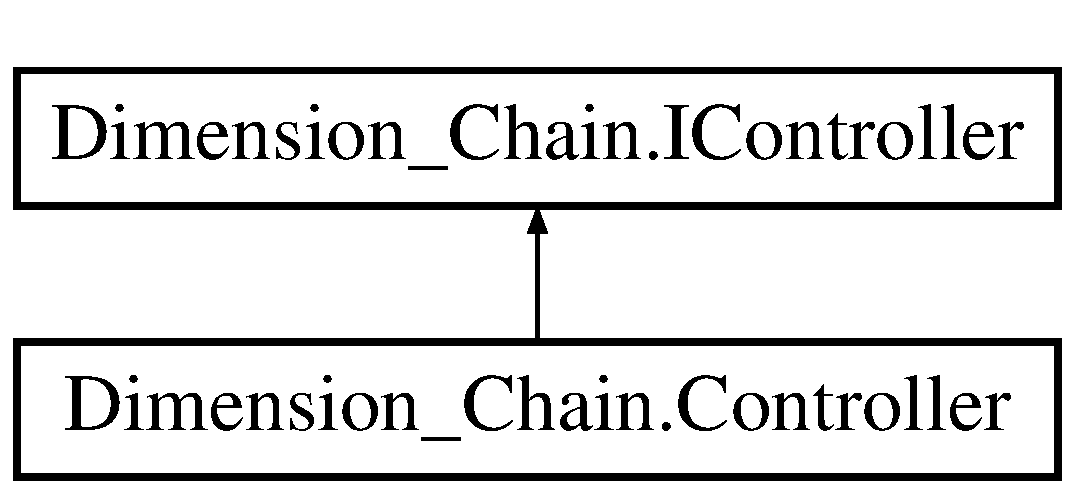
\includegraphics[height=2.000000cm]{interface_dimension___chain_1_1_i_controller}
\end{center}
\end{figure}
\subsection*{Public Member Functions}
\begin{DoxyCompactItemize}
\item 
bool \mbox{\hyperlink{interface_dimension___chain_1_1_i_controller_a228ee16ef616fee00fc5141e3ebef9db}{is\+Create\+Dimension}} ()
\end{DoxyCompactItemize}


\subsection{Member Function Documentation}
\mbox{\Hypertarget{interface_dimension___chain_1_1_i_controller_a228ee16ef616fee00fc5141e3ebef9db}\label{interface_dimension___chain_1_1_i_controller_a228ee16ef616fee00fc5141e3ebef9db}} 
\index{Dimension\+\_\+\+Chain\+::\+I\+Controller@{Dimension\+\_\+\+Chain\+::\+I\+Controller}!is\+Create\+Dimension@{is\+Create\+Dimension}}
\index{is\+Create\+Dimension@{is\+Create\+Dimension}!Dimension\+\_\+\+Chain\+::\+I\+Controller@{Dimension\+\_\+\+Chain\+::\+I\+Controller}}
\subsubsection{\texorpdfstring{is\+Create\+Dimension()}{isCreateDimension()}}
{\footnotesize\ttfamily bool Dimension\+\_\+\+Chain.\+I\+Controller.\+is\+Create\+Dimension (\begin{DoxyParamCaption}{ }\end{DoxyParamCaption})}



Implemented in \mbox{\hyperlink{class_dimension___chain_1_1_controller_ae8c6a98ffe1507c958ca65e93d533c87}{Dimension\+\_\+\+Chain.\+Controller}}.



The documentation for this interface was generated from the following file\+:\begin{DoxyCompactItemize}
\item 
\mbox{\hyperlink{_controller_8cs}{Controller.\+cs}}\end{DoxyCompactItemize}

\hypertarget{class_dimension___chain_1_1_main_window}{}\section{Dimension\+\_\+\+Chain.\+Main\+Window Class Reference}
\label{class_dimension___chain_1_1_main_window}\index{Dimension\+\_\+\+Chain.\+Main\+Window@{Dimension\+\_\+\+Chain.\+Main\+Window}}


Логика взаимодействия для Main\+Window.\+xaml -\/ V\+I\+EW  


Inheritance diagram for Dimension\+\_\+\+Chain.\+Main\+Window\+:\begin{figure}[H]
\begin{center}
\leavevmode
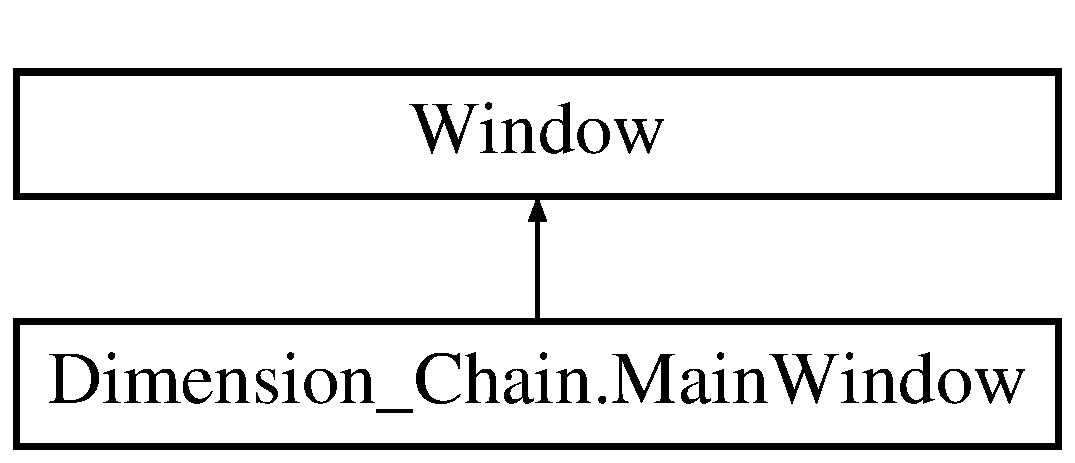
\includegraphics[height=2.000000cm]{class_dimension___chain_1_1_main_window}
\end{center}
\end{figure}
\subsection*{Public Member Functions}
\begin{DoxyCompactItemize}
\item 
delegate void \mbox{\hyperlink{class_dimension___chain_1_1_main_window_a34a91a946df99f170f8961d961a1fa8f}{Del\+Pressed\+Event\+Handler}} ()
\item 
delegate void \mbox{\hyperlink{class_dimension___chain_1_1_main_window_acfa98ee5bdb96cc53214007d560dd087}{Esc\+Pressed\+Event\+Handler}} ()
\item 
delegate void \mbox{\hyperlink{class_dimension___chain_1_1_main_window_ad49f6daca6cd98a445ca9d17d46b04ee}{Wheel\+Event\+Handler}} (Point p)
\item 
delegate void \mbox{\hyperlink{class_dimension___chain_1_1_main_window_a8474fa1057f9cae2aa47066564dc69ee}{Mouse\+Left\+Button\+Down\+On\+Canvas\+Event\+Handler}} ()
\item 
delegate void \mbox{\hyperlink{class_dimension___chain_1_1_main_window_a91ca9eba3ad3e48423c7a28f4fa5bcc2}{Save\+Event\+Handler}} ()
\item 
delegate void \mbox{\hyperlink{class_dimension___chain_1_1_main_window_aad640b4de47e0ac6ac018cc8e612a792}{Open\+Event\+Handler}} ()
\item 
delegate void \mbox{\hyperlink{class_dimension___chain_1_1_main_window_a973bbb7ae10c9591b950d4b1b5d9eea3}{New\+Project\+Event\+Handler}} ()
\item 
\mbox{\hyperlink{class_dimension___chain_1_1_main_window_a0ebc5549460f612ea2a5072bf25e5178}{Main\+Window}} ()
\item 
void \mbox{\hyperlink{class_dimension___chain_1_1_main_window_a77a7bface86a04e6f19dd6071437dd3b}{Set\+Save\+Enable}} (bool is\+Enabled)
\end{DoxyCompactItemize}
\subsection*{Static Public Attributes}
\begin{DoxyCompactItemize}
\item 
static Text\+Box \mbox{\hyperlink{class_dimension___chain_1_1_main_window_ac9471cc1c0e1856c8d4602c21ca6fc1b}{test\+TB}}
\end{DoxyCompactItemize}
\subsection*{Events}
\begin{DoxyCompactItemize}
\item 
static \mbox{\hyperlink{class_dimension___chain_1_1_main_window_a34a91a946df99f170f8961d961a1fa8f}{Del\+Pressed\+Event\+Handler}} \mbox{\hyperlink{class_dimension___chain_1_1_main_window_add4063327d2d2bca0a70fa0040dc6ee5}{Del\+Pressed}}
\item 
static \mbox{\hyperlink{class_dimension___chain_1_1_main_window_acfa98ee5bdb96cc53214007d560dd087}{Esc\+Pressed\+Event\+Handler}} \mbox{\hyperlink{class_dimension___chain_1_1_main_window_a2587a8d2c35cf0e2722dd0704ca4c763}{Esc\+Pressed}}
\item 
static \mbox{\hyperlink{class_dimension___chain_1_1_main_window_ad49f6daca6cd98a445ca9d17d46b04ee}{Wheel\+Event\+Handler}} \mbox{\hyperlink{class_dimension___chain_1_1_main_window_a03c4a933fc8b36209bd22ef959ba87a2}{Wheel\+Up}}
\item 
static \mbox{\hyperlink{class_dimension___chain_1_1_main_window_ad49f6daca6cd98a445ca9d17d46b04ee}{Wheel\+Event\+Handler}} \mbox{\hyperlink{class_dimension___chain_1_1_main_window_a5b9d3178e029918e243295f9f7bdf21a}{Wheel\+Down}}
\item 
static \mbox{\hyperlink{class_dimension___chain_1_1_main_window_a8474fa1057f9cae2aa47066564dc69ee}{Mouse\+Left\+Button\+Down\+On\+Canvas\+Event\+Handler}} \mbox{\hyperlink{class_dimension___chain_1_1_main_window_a375f69d6d40a39909d9298824d7cf133}{Mouse\+Left\+Button\+Down\+On\+Canvas}}
\item 
static \mbox{\hyperlink{class_dimension___chain_1_1_main_window_a91ca9eba3ad3e48423c7a28f4fa5bcc2}{Save\+Event\+Handler}} \mbox{\hyperlink{class_dimension___chain_1_1_main_window_a631b06f923cbd0704faa23ba6abc381c}{Save\+All\+As}}
\item 
static \mbox{\hyperlink{class_dimension___chain_1_1_main_window_a91ca9eba3ad3e48423c7a28f4fa5bcc2}{Save\+Event\+Handler}} \mbox{\hyperlink{class_dimension___chain_1_1_main_window_a121618b4d573a4127931b905ff7bdee4}{Save\+All}}
\item 
static \mbox{\hyperlink{class_dimension___chain_1_1_main_window_aad640b4de47e0ac6ac018cc8e612a792}{Open\+Event\+Handler}} \mbox{\hyperlink{class_dimension___chain_1_1_main_window_a800583b52dc2b7c26852d45bfab4b73f}{Open\+Saved}}
\item 
static \mbox{\hyperlink{class_dimension___chain_1_1_main_window_a973bbb7ae10c9591b950d4b1b5d9eea3}{New\+Project\+Event\+Handler}} \mbox{\hyperlink{class_dimension___chain_1_1_main_window_adf110c4fad0a5ccd89268bd6ce7f675c}{New\+Proj}}
\end{DoxyCompactItemize}


\subsection{Detailed Description}
Логика взаимодействия для Main\+Window.\+xaml -\/ V\+I\+EW 



\subsection{Constructor \& Destructor Documentation}
\mbox{\Hypertarget{class_dimension___chain_1_1_main_window_a0ebc5549460f612ea2a5072bf25e5178}\label{class_dimension___chain_1_1_main_window_a0ebc5549460f612ea2a5072bf25e5178}} 
\index{Dimension\+\_\+\+Chain\+::\+Main\+Window@{Dimension\+\_\+\+Chain\+::\+Main\+Window}!Main\+Window@{Main\+Window}}
\index{Main\+Window@{Main\+Window}!Dimension\+\_\+\+Chain\+::\+Main\+Window@{Dimension\+\_\+\+Chain\+::\+Main\+Window}}
\subsubsection{\texorpdfstring{Main\+Window()}{MainWindow()}}
{\footnotesize\ttfamily Dimension\+\_\+\+Chain.\+Main\+Window.\+Main\+Window (\begin{DoxyParamCaption}{ }\end{DoxyParamCaption})}



\subsection{Member Function Documentation}
\mbox{\Hypertarget{class_dimension___chain_1_1_main_window_a34a91a946df99f170f8961d961a1fa8f}\label{class_dimension___chain_1_1_main_window_a34a91a946df99f170f8961d961a1fa8f}} 
\index{Dimension\+\_\+\+Chain\+::\+Main\+Window@{Dimension\+\_\+\+Chain\+::\+Main\+Window}!Del\+Pressed\+Event\+Handler@{Del\+Pressed\+Event\+Handler}}
\index{Del\+Pressed\+Event\+Handler@{Del\+Pressed\+Event\+Handler}!Dimension\+\_\+\+Chain\+::\+Main\+Window@{Dimension\+\_\+\+Chain\+::\+Main\+Window}}
\subsubsection{\texorpdfstring{Del\+Pressed\+Event\+Handler()}{DelPressedEventHandler()}}
{\footnotesize\ttfamily delegate void Dimension\+\_\+\+Chain.\+Main\+Window.\+Del\+Pressed\+Event\+Handler (\begin{DoxyParamCaption}{ }\end{DoxyParamCaption})}

\mbox{\Hypertarget{class_dimension___chain_1_1_main_window_acfa98ee5bdb96cc53214007d560dd087}\label{class_dimension___chain_1_1_main_window_acfa98ee5bdb96cc53214007d560dd087}} 
\index{Dimension\+\_\+\+Chain\+::\+Main\+Window@{Dimension\+\_\+\+Chain\+::\+Main\+Window}!Esc\+Pressed\+Event\+Handler@{Esc\+Pressed\+Event\+Handler}}
\index{Esc\+Pressed\+Event\+Handler@{Esc\+Pressed\+Event\+Handler}!Dimension\+\_\+\+Chain\+::\+Main\+Window@{Dimension\+\_\+\+Chain\+::\+Main\+Window}}
\subsubsection{\texorpdfstring{Esc\+Pressed\+Event\+Handler()}{EscPressedEventHandler()}}
{\footnotesize\ttfamily delegate void Dimension\+\_\+\+Chain.\+Main\+Window.\+Esc\+Pressed\+Event\+Handler (\begin{DoxyParamCaption}{ }\end{DoxyParamCaption})}

\mbox{\Hypertarget{class_dimension___chain_1_1_main_window_a8474fa1057f9cae2aa47066564dc69ee}\label{class_dimension___chain_1_1_main_window_a8474fa1057f9cae2aa47066564dc69ee}} 
\index{Dimension\+\_\+\+Chain\+::\+Main\+Window@{Dimension\+\_\+\+Chain\+::\+Main\+Window}!Mouse\+Left\+Button\+Down\+On\+Canvas\+Event\+Handler@{Mouse\+Left\+Button\+Down\+On\+Canvas\+Event\+Handler}}
\index{Mouse\+Left\+Button\+Down\+On\+Canvas\+Event\+Handler@{Mouse\+Left\+Button\+Down\+On\+Canvas\+Event\+Handler}!Dimension\+\_\+\+Chain\+::\+Main\+Window@{Dimension\+\_\+\+Chain\+::\+Main\+Window}}
\subsubsection{\texorpdfstring{Mouse\+Left\+Button\+Down\+On\+Canvas\+Event\+Handler()}{MouseLeftButtonDownOnCanvasEventHandler()}}
{\footnotesize\ttfamily delegate void Dimension\+\_\+\+Chain.\+Main\+Window.\+Mouse\+Left\+Button\+Down\+On\+Canvas\+Event\+Handler (\begin{DoxyParamCaption}{ }\end{DoxyParamCaption})}

\mbox{\Hypertarget{class_dimension___chain_1_1_main_window_a973bbb7ae10c9591b950d4b1b5d9eea3}\label{class_dimension___chain_1_1_main_window_a973bbb7ae10c9591b950d4b1b5d9eea3}} 
\index{Dimension\+\_\+\+Chain\+::\+Main\+Window@{Dimension\+\_\+\+Chain\+::\+Main\+Window}!New\+Project\+Event\+Handler@{New\+Project\+Event\+Handler}}
\index{New\+Project\+Event\+Handler@{New\+Project\+Event\+Handler}!Dimension\+\_\+\+Chain\+::\+Main\+Window@{Dimension\+\_\+\+Chain\+::\+Main\+Window}}
\subsubsection{\texorpdfstring{New\+Project\+Event\+Handler()}{NewProjectEventHandler()}}
{\footnotesize\ttfamily delegate void Dimension\+\_\+\+Chain.\+Main\+Window.\+New\+Project\+Event\+Handler (\begin{DoxyParamCaption}{ }\end{DoxyParamCaption})}

\mbox{\Hypertarget{class_dimension___chain_1_1_main_window_aad640b4de47e0ac6ac018cc8e612a792}\label{class_dimension___chain_1_1_main_window_aad640b4de47e0ac6ac018cc8e612a792}} 
\index{Dimension\+\_\+\+Chain\+::\+Main\+Window@{Dimension\+\_\+\+Chain\+::\+Main\+Window}!Open\+Event\+Handler@{Open\+Event\+Handler}}
\index{Open\+Event\+Handler@{Open\+Event\+Handler}!Dimension\+\_\+\+Chain\+::\+Main\+Window@{Dimension\+\_\+\+Chain\+::\+Main\+Window}}
\subsubsection{\texorpdfstring{Open\+Event\+Handler()}{OpenEventHandler()}}
{\footnotesize\ttfamily delegate void Dimension\+\_\+\+Chain.\+Main\+Window.\+Open\+Event\+Handler (\begin{DoxyParamCaption}{ }\end{DoxyParamCaption})}

\mbox{\Hypertarget{class_dimension___chain_1_1_main_window_a91ca9eba3ad3e48423c7a28f4fa5bcc2}\label{class_dimension___chain_1_1_main_window_a91ca9eba3ad3e48423c7a28f4fa5bcc2}} 
\index{Dimension\+\_\+\+Chain\+::\+Main\+Window@{Dimension\+\_\+\+Chain\+::\+Main\+Window}!Save\+Event\+Handler@{Save\+Event\+Handler}}
\index{Save\+Event\+Handler@{Save\+Event\+Handler}!Dimension\+\_\+\+Chain\+::\+Main\+Window@{Dimension\+\_\+\+Chain\+::\+Main\+Window}}
\subsubsection{\texorpdfstring{Save\+Event\+Handler()}{SaveEventHandler()}}
{\footnotesize\ttfamily delegate void Dimension\+\_\+\+Chain.\+Main\+Window.\+Save\+Event\+Handler (\begin{DoxyParamCaption}{ }\end{DoxyParamCaption})}

\mbox{\Hypertarget{class_dimension___chain_1_1_main_window_a77a7bface86a04e6f19dd6071437dd3b}\label{class_dimension___chain_1_1_main_window_a77a7bface86a04e6f19dd6071437dd3b}} 
\index{Dimension\+\_\+\+Chain\+::\+Main\+Window@{Dimension\+\_\+\+Chain\+::\+Main\+Window}!Set\+Save\+Enable@{Set\+Save\+Enable}}
\index{Set\+Save\+Enable@{Set\+Save\+Enable}!Dimension\+\_\+\+Chain\+::\+Main\+Window@{Dimension\+\_\+\+Chain\+::\+Main\+Window}}
\subsubsection{\texorpdfstring{Set\+Save\+Enable()}{SetSaveEnable()}}
{\footnotesize\ttfamily void Dimension\+\_\+\+Chain.\+Main\+Window.\+Set\+Save\+Enable (\begin{DoxyParamCaption}\item[{bool}]{is\+Enabled }\end{DoxyParamCaption})}

\mbox{\Hypertarget{class_dimension___chain_1_1_main_window_ad49f6daca6cd98a445ca9d17d46b04ee}\label{class_dimension___chain_1_1_main_window_ad49f6daca6cd98a445ca9d17d46b04ee}} 
\index{Dimension\+\_\+\+Chain\+::\+Main\+Window@{Dimension\+\_\+\+Chain\+::\+Main\+Window}!Wheel\+Event\+Handler@{Wheel\+Event\+Handler}}
\index{Wheel\+Event\+Handler@{Wheel\+Event\+Handler}!Dimension\+\_\+\+Chain\+::\+Main\+Window@{Dimension\+\_\+\+Chain\+::\+Main\+Window}}
\subsubsection{\texorpdfstring{Wheel\+Event\+Handler()}{WheelEventHandler()}}
{\footnotesize\ttfamily delegate void Dimension\+\_\+\+Chain.\+Main\+Window.\+Wheel\+Event\+Handler (\begin{DoxyParamCaption}\item[{Point}]{p }\end{DoxyParamCaption})}



\subsection{Member Data Documentation}
\mbox{\Hypertarget{class_dimension___chain_1_1_main_window_ac9471cc1c0e1856c8d4602c21ca6fc1b}\label{class_dimension___chain_1_1_main_window_ac9471cc1c0e1856c8d4602c21ca6fc1b}} 
\index{Dimension\+\_\+\+Chain\+::\+Main\+Window@{Dimension\+\_\+\+Chain\+::\+Main\+Window}!test\+TB@{test\+TB}}
\index{test\+TB@{test\+TB}!Dimension\+\_\+\+Chain\+::\+Main\+Window@{Dimension\+\_\+\+Chain\+::\+Main\+Window}}
\subsubsection{\texorpdfstring{test\+TB}{testTB}}
{\footnotesize\ttfamily Text\+Box Dimension\+\_\+\+Chain.\+Main\+Window.\+test\+TB\hspace{0.3cm}{\ttfamily [static]}}



\subsection{Event Documentation}
\mbox{\Hypertarget{class_dimension___chain_1_1_main_window_add4063327d2d2bca0a70fa0040dc6ee5}\label{class_dimension___chain_1_1_main_window_add4063327d2d2bca0a70fa0040dc6ee5}} 
\index{Dimension\+\_\+\+Chain\+::\+Main\+Window@{Dimension\+\_\+\+Chain\+::\+Main\+Window}!Del\+Pressed@{Del\+Pressed}}
\index{Del\+Pressed@{Del\+Pressed}!Dimension\+\_\+\+Chain\+::\+Main\+Window@{Dimension\+\_\+\+Chain\+::\+Main\+Window}}
\subsubsection{\texorpdfstring{Del\+Pressed}{DelPressed}}
{\footnotesize\ttfamily \mbox{\hyperlink{class_dimension___chain_1_1_main_window_a34a91a946df99f170f8961d961a1fa8f}{Del\+Pressed\+Event\+Handler}} Dimension\+\_\+\+Chain.\+Main\+Window.\+Del\+Pressed\hspace{0.3cm}{\ttfamily [static]}}

\mbox{\Hypertarget{class_dimension___chain_1_1_main_window_a2587a8d2c35cf0e2722dd0704ca4c763}\label{class_dimension___chain_1_1_main_window_a2587a8d2c35cf0e2722dd0704ca4c763}} 
\index{Dimension\+\_\+\+Chain\+::\+Main\+Window@{Dimension\+\_\+\+Chain\+::\+Main\+Window}!Esc\+Pressed@{Esc\+Pressed}}
\index{Esc\+Pressed@{Esc\+Pressed}!Dimension\+\_\+\+Chain\+::\+Main\+Window@{Dimension\+\_\+\+Chain\+::\+Main\+Window}}
\subsubsection{\texorpdfstring{Esc\+Pressed}{EscPressed}}
{\footnotesize\ttfamily \mbox{\hyperlink{class_dimension___chain_1_1_main_window_acfa98ee5bdb96cc53214007d560dd087}{Esc\+Pressed\+Event\+Handler}} Dimension\+\_\+\+Chain.\+Main\+Window.\+Esc\+Pressed\hspace{0.3cm}{\ttfamily [static]}}

\mbox{\Hypertarget{class_dimension___chain_1_1_main_window_a375f69d6d40a39909d9298824d7cf133}\label{class_dimension___chain_1_1_main_window_a375f69d6d40a39909d9298824d7cf133}} 
\index{Dimension\+\_\+\+Chain\+::\+Main\+Window@{Dimension\+\_\+\+Chain\+::\+Main\+Window}!Mouse\+Left\+Button\+Down\+On\+Canvas@{Mouse\+Left\+Button\+Down\+On\+Canvas}}
\index{Mouse\+Left\+Button\+Down\+On\+Canvas@{Mouse\+Left\+Button\+Down\+On\+Canvas}!Dimension\+\_\+\+Chain\+::\+Main\+Window@{Dimension\+\_\+\+Chain\+::\+Main\+Window}}
\subsubsection{\texorpdfstring{Mouse\+Left\+Button\+Down\+On\+Canvas}{MouseLeftButtonDownOnCanvas}}
{\footnotesize\ttfamily \mbox{\hyperlink{class_dimension___chain_1_1_main_window_a8474fa1057f9cae2aa47066564dc69ee}{Mouse\+Left\+Button\+Down\+On\+Canvas\+Event\+Handler}} Dimension\+\_\+\+Chain.\+Main\+Window.\+Mouse\+Left\+Button\+Down\+On\+Canvas\hspace{0.3cm}{\ttfamily [static]}}

\mbox{\Hypertarget{class_dimension___chain_1_1_main_window_adf110c4fad0a5ccd89268bd6ce7f675c}\label{class_dimension___chain_1_1_main_window_adf110c4fad0a5ccd89268bd6ce7f675c}} 
\index{Dimension\+\_\+\+Chain\+::\+Main\+Window@{Dimension\+\_\+\+Chain\+::\+Main\+Window}!New\+Proj@{New\+Proj}}
\index{New\+Proj@{New\+Proj}!Dimension\+\_\+\+Chain\+::\+Main\+Window@{Dimension\+\_\+\+Chain\+::\+Main\+Window}}
\subsubsection{\texorpdfstring{New\+Proj}{NewProj}}
{\footnotesize\ttfamily \mbox{\hyperlink{class_dimension___chain_1_1_main_window_a973bbb7ae10c9591b950d4b1b5d9eea3}{New\+Project\+Event\+Handler}} Dimension\+\_\+\+Chain.\+Main\+Window.\+New\+Proj\hspace{0.3cm}{\ttfamily [static]}}

\mbox{\Hypertarget{class_dimension___chain_1_1_main_window_a800583b52dc2b7c26852d45bfab4b73f}\label{class_dimension___chain_1_1_main_window_a800583b52dc2b7c26852d45bfab4b73f}} 
\index{Dimension\+\_\+\+Chain\+::\+Main\+Window@{Dimension\+\_\+\+Chain\+::\+Main\+Window}!Open\+Saved@{Open\+Saved}}
\index{Open\+Saved@{Open\+Saved}!Dimension\+\_\+\+Chain\+::\+Main\+Window@{Dimension\+\_\+\+Chain\+::\+Main\+Window}}
\subsubsection{\texorpdfstring{Open\+Saved}{OpenSaved}}
{\footnotesize\ttfamily \mbox{\hyperlink{class_dimension___chain_1_1_main_window_aad640b4de47e0ac6ac018cc8e612a792}{Open\+Event\+Handler}} Dimension\+\_\+\+Chain.\+Main\+Window.\+Open\+Saved\hspace{0.3cm}{\ttfamily [static]}}

\mbox{\Hypertarget{class_dimension___chain_1_1_main_window_a121618b4d573a4127931b905ff7bdee4}\label{class_dimension___chain_1_1_main_window_a121618b4d573a4127931b905ff7bdee4}} 
\index{Dimension\+\_\+\+Chain\+::\+Main\+Window@{Dimension\+\_\+\+Chain\+::\+Main\+Window}!Save\+All@{Save\+All}}
\index{Save\+All@{Save\+All}!Dimension\+\_\+\+Chain\+::\+Main\+Window@{Dimension\+\_\+\+Chain\+::\+Main\+Window}}
\subsubsection{\texorpdfstring{Save\+All}{SaveAll}}
{\footnotesize\ttfamily \mbox{\hyperlink{class_dimension___chain_1_1_main_window_a91ca9eba3ad3e48423c7a28f4fa5bcc2}{Save\+Event\+Handler}} Dimension\+\_\+\+Chain.\+Main\+Window.\+Save\+All\hspace{0.3cm}{\ttfamily [static]}}

\mbox{\Hypertarget{class_dimension___chain_1_1_main_window_a631b06f923cbd0704faa23ba6abc381c}\label{class_dimension___chain_1_1_main_window_a631b06f923cbd0704faa23ba6abc381c}} 
\index{Dimension\+\_\+\+Chain\+::\+Main\+Window@{Dimension\+\_\+\+Chain\+::\+Main\+Window}!Save\+All\+As@{Save\+All\+As}}
\index{Save\+All\+As@{Save\+All\+As}!Dimension\+\_\+\+Chain\+::\+Main\+Window@{Dimension\+\_\+\+Chain\+::\+Main\+Window}}
\subsubsection{\texorpdfstring{Save\+All\+As}{SaveAllAs}}
{\footnotesize\ttfamily \mbox{\hyperlink{class_dimension___chain_1_1_main_window_a91ca9eba3ad3e48423c7a28f4fa5bcc2}{Save\+Event\+Handler}} Dimension\+\_\+\+Chain.\+Main\+Window.\+Save\+All\+As\hspace{0.3cm}{\ttfamily [static]}}

\mbox{\Hypertarget{class_dimension___chain_1_1_main_window_a5b9d3178e029918e243295f9f7bdf21a}\label{class_dimension___chain_1_1_main_window_a5b9d3178e029918e243295f9f7bdf21a}} 
\index{Dimension\+\_\+\+Chain\+::\+Main\+Window@{Dimension\+\_\+\+Chain\+::\+Main\+Window}!Wheel\+Down@{Wheel\+Down}}
\index{Wheel\+Down@{Wheel\+Down}!Dimension\+\_\+\+Chain\+::\+Main\+Window@{Dimension\+\_\+\+Chain\+::\+Main\+Window}}
\subsubsection{\texorpdfstring{Wheel\+Down}{WheelDown}}
{\footnotesize\ttfamily \mbox{\hyperlink{class_dimension___chain_1_1_main_window_ad49f6daca6cd98a445ca9d17d46b04ee}{Wheel\+Event\+Handler}} Dimension\+\_\+\+Chain.\+Main\+Window.\+Wheel\+Down\hspace{0.3cm}{\ttfamily [static]}}

\mbox{\Hypertarget{class_dimension___chain_1_1_main_window_a03c4a933fc8b36209bd22ef959ba87a2}\label{class_dimension___chain_1_1_main_window_a03c4a933fc8b36209bd22ef959ba87a2}} 
\index{Dimension\+\_\+\+Chain\+::\+Main\+Window@{Dimension\+\_\+\+Chain\+::\+Main\+Window}!Wheel\+Up@{Wheel\+Up}}
\index{Wheel\+Up@{Wheel\+Up}!Dimension\+\_\+\+Chain\+::\+Main\+Window@{Dimension\+\_\+\+Chain\+::\+Main\+Window}}
\subsubsection{\texorpdfstring{Wheel\+Up}{WheelUp}}
{\footnotesize\ttfamily \mbox{\hyperlink{class_dimension___chain_1_1_main_window_ad49f6daca6cd98a445ca9d17d46b04ee}{Wheel\+Event\+Handler}} Dimension\+\_\+\+Chain.\+Main\+Window.\+Wheel\+Up\hspace{0.3cm}{\ttfamily [static]}}



The documentation for this class was generated from the following file\+:\begin{DoxyCompactItemize}
\item 
\mbox{\hyperlink{_main_window_8xaml_8cs}{Main\+Window.\+xaml.\+cs}}\end{DoxyCompactItemize}

\hypertarget{class_dimension___chain_1_1_mega_vertex}{}\section{Dimension\+\_\+\+Chain.\+Mega\+Vertex Class Reference}
\label{class_dimension___chain_1_1_mega_vertex}\index{Dimension\+\_\+\+Chain.\+Mega\+Vertex@{Dimension\+\_\+\+Chain.\+Mega\+Vertex}}
\subsection*{Public Attributes}
\begin{DoxyCompactItemize}
\item 
List$<$ \mbox{\hyperlink{class_dimension___chain_1_1_vertex}{Vertex}} $>$ \mbox{\hyperlink{class_dimension___chain_1_1_mega_vertex_a6436cd17c7b224a2f5bc70706ab1e113}{vertex\+List}} = new List$<$\mbox{\hyperlink{class_dimension___chain_1_1_vertex}{Vertex}}$>$()
\item 
List$<$ \mbox{\hyperlink{class_dimension___chain_1_1_mega_vertex}{Mega\+Vertex}} $>$ \mbox{\hyperlink{class_dimension___chain_1_1_mega_vertex_ab0e8d9f1b5bcd0250a4eb0af29474dbd}{neighbors}} = new List$<$\mbox{\hyperlink{class_dimension___chain_1_1_mega_vertex}{Mega\+Vertex}}$>$()
\item 
bool \mbox{\hyperlink{class_dimension___chain_1_1_mega_vertex_a3b3d1b34b302a30828f1402a62c01004}{visited}} = false
\end{DoxyCompactItemize}


\subsection{Member Data Documentation}
\mbox{\Hypertarget{class_dimension___chain_1_1_mega_vertex_ab0e8d9f1b5bcd0250a4eb0af29474dbd}\label{class_dimension___chain_1_1_mega_vertex_ab0e8d9f1b5bcd0250a4eb0af29474dbd}} 
\index{Dimension\+\_\+\+Chain\+::\+Mega\+Vertex@{Dimension\+\_\+\+Chain\+::\+Mega\+Vertex}!neighbors@{neighbors}}
\index{neighbors@{neighbors}!Dimension\+\_\+\+Chain\+::\+Mega\+Vertex@{Dimension\+\_\+\+Chain\+::\+Mega\+Vertex}}
\subsubsection{\texorpdfstring{neighbors}{neighbors}}
{\footnotesize\ttfamily List$<$\mbox{\hyperlink{class_dimension___chain_1_1_mega_vertex}{Mega\+Vertex}}$>$ Dimension\+\_\+\+Chain.\+Mega\+Vertex.\+neighbors = new List$<$\mbox{\hyperlink{class_dimension___chain_1_1_mega_vertex}{Mega\+Vertex}}$>$()}

\mbox{\Hypertarget{class_dimension___chain_1_1_mega_vertex_a6436cd17c7b224a2f5bc70706ab1e113}\label{class_dimension___chain_1_1_mega_vertex_a6436cd17c7b224a2f5bc70706ab1e113}} 
\index{Dimension\+\_\+\+Chain\+::\+Mega\+Vertex@{Dimension\+\_\+\+Chain\+::\+Mega\+Vertex}!vertex\+List@{vertex\+List}}
\index{vertex\+List@{vertex\+List}!Dimension\+\_\+\+Chain\+::\+Mega\+Vertex@{Dimension\+\_\+\+Chain\+::\+Mega\+Vertex}}
\subsubsection{\texorpdfstring{vertex\+List}{vertexList}}
{\footnotesize\ttfamily List$<$\mbox{\hyperlink{class_dimension___chain_1_1_vertex}{Vertex}}$>$ Dimension\+\_\+\+Chain.\+Mega\+Vertex.\+vertex\+List = new List$<$\mbox{\hyperlink{class_dimension___chain_1_1_vertex}{Vertex}}$>$()}

\mbox{\Hypertarget{class_dimension___chain_1_1_mega_vertex_a3b3d1b34b302a30828f1402a62c01004}\label{class_dimension___chain_1_1_mega_vertex_a3b3d1b34b302a30828f1402a62c01004}} 
\index{Dimension\+\_\+\+Chain\+::\+Mega\+Vertex@{Dimension\+\_\+\+Chain\+::\+Mega\+Vertex}!visited@{visited}}
\index{visited@{visited}!Dimension\+\_\+\+Chain\+::\+Mega\+Vertex@{Dimension\+\_\+\+Chain\+::\+Mega\+Vertex}}
\subsubsection{\texorpdfstring{visited}{visited}}
{\footnotesize\ttfamily bool Dimension\+\_\+\+Chain.\+Mega\+Vertex.\+visited = false}



The documentation for this class was generated from the following file\+:\begin{DoxyCompactItemize}
\item 
\mbox{\hyperlink{_mega_vertex_8cs}{Mega\+Vertex.\+cs}}\end{DoxyCompactItemize}

\hypertarget{class_dimension___chain_1_1_native_methods}{}\section{Dimension\+\_\+\+Chain.\+Native\+Methods Class Reference}
\label{class_dimension___chain_1_1_native_methods}\index{Dimension\+\_\+\+Chain.\+Native\+Methods@{Dimension\+\_\+\+Chain.\+Native\+Methods}}
\subsection*{Public Member Functions}
\begin{DoxyCompactItemize}
\item 
static bool \mbox{\hyperlink{class_dimension___chain_1_1_native_methods_ab0debd810a872bbc9c47448dd23c0ff3}{Set\+Cursor\+Pos}} (int X, int Y)
\end{DoxyCompactItemize}


\subsection{Member Function Documentation}
\mbox{\Hypertarget{class_dimension___chain_1_1_native_methods_ab0debd810a872bbc9c47448dd23c0ff3}\label{class_dimension___chain_1_1_native_methods_ab0debd810a872bbc9c47448dd23c0ff3}} 
\index{Dimension\+\_\+\+Chain\+::\+Native\+Methods@{Dimension\+\_\+\+Chain\+::\+Native\+Methods}!Set\+Cursor\+Pos@{Set\+Cursor\+Pos}}
\index{Set\+Cursor\+Pos@{Set\+Cursor\+Pos}!Dimension\+\_\+\+Chain\+::\+Native\+Methods@{Dimension\+\_\+\+Chain\+::\+Native\+Methods}}
\subsubsection{\texorpdfstring{Set\+Cursor\+Pos()}{SetCursorPos()}}
{\footnotesize\ttfamily static bool Dimension\+\_\+\+Chain.\+Native\+Methods.\+Set\+Cursor\+Pos (\begin{DoxyParamCaption}\item[{int}]{X,  }\item[{int}]{Y }\end{DoxyParamCaption})}

Return Type\+: B\+O\+O\+L-\/$>$int ~\newline
X\+: int ~\newline
Y\+: int 

The documentation for this class was generated from the following file\+:\begin{DoxyCompactItemize}
\item 
\mbox{\hyperlink{_u_i___dimension_8cs}{U\+I\+\_\+\+Dimension.\+cs}}\end{DoxyCompactItemize}

\hypertarget{class_dimension___chain_1_1_pripusk_user_control}{}\section{Dimension\+\_\+\+Chain.\+Pripusk\+User\+Control Class Reference}
\label{class_dimension___chain_1_1_pripusk_user_control}\index{Dimension\+\_\+\+Chain.\+Pripusk\+User\+Control@{Dimension\+\_\+\+Chain.\+Pripusk\+User\+Control}}


Логика взаимодействия для Pripusk\+User\+Control.\+xaml  


Inheritance diagram for Dimension\+\_\+\+Chain.\+Pripusk\+User\+Control\+:\begin{figure}[H]
\begin{center}
\leavevmode
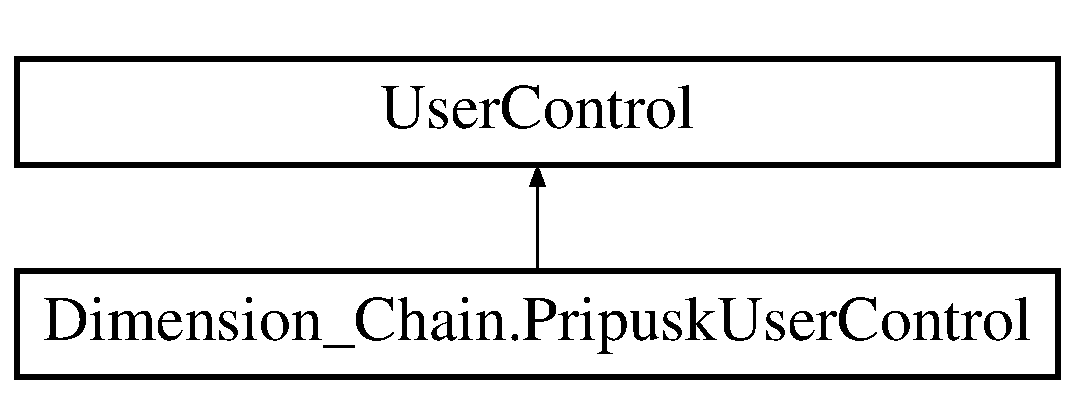
\includegraphics[height=2.000000cm]{class_dimension___chain_1_1_pripusk_user_control}
\end{center}
\end{figure}
\subsection*{Public Member Functions}
\begin{DoxyCompactItemize}
\item 
\mbox{\hyperlink{class_dimension___chain_1_1_pripusk_user_control_a47b71047602454b227feb662ca976281}{Pripusk\+User\+Control}} ()
\item 
void \mbox{\hyperlink{class_dimension___chain_1_1_pripusk_user_control_a4907b2646788dd49f089d3e1e2fd6af4}{Set\+U\+I\+\_\+\+PD}} (\mbox{\hyperlink{class_dimension___chain_1_1_u_i___pripusk_dimension}{U\+I\+\_\+\+Pripusk\+Dimension}} U\+I\+\_\+\+PD)
\item 
void \mbox{\hyperlink{class_dimension___chain_1_1_pripusk_user_control_a15805f1227585bd517f428f0c773d803}{Re\+Null}} ()
\end{DoxyCompactItemize}


\subsection{Detailed Description}
Логика взаимодействия для Pripusk\+User\+Control.\+xaml 



\subsection{Constructor \& Destructor Documentation}
\mbox{\Hypertarget{class_dimension___chain_1_1_pripusk_user_control_a47b71047602454b227feb662ca976281}\label{class_dimension___chain_1_1_pripusk_user_control_a47b71047602454b227feb662ca976281}} 
\index{Dimension\+\_\+\+Chain\+::\+Pripusk\+User\+Control@{Dimension\+\_\+\+Chain\+::\+Pripusk\+User\+Control}!Pripusk\+User\+Control@{Pripusk\+User\+Control}}
\index{Pripusk\+User\+Control@{Pripusk\+User\+Control}!Dimension\+\_\+\+Chain\+::\+Pripusk\+User\+Control@{Dimension\+\_\+\+Chain\+::\+Pripusk\+User\+Control}}
\subsubsection{\texorpdfstring{Pripusk\+User\+Control()}{PripuskUserControl()}}
{\footnotesize\ttfamily Dimension\+\_\+\+Chain.\+Pripusk\+User\+Control.\+Pripusk\+User\+Control (\begin{DoxyParamCaption}{ }\end{DoxyParamCaption})}



\subsection{Member Function Documentation}
\mbox{\Hypertarget{class_dimension___chain_1_1_pripusk_user_control_a15805f1227585bd517f428f0c773d803}\label{class_dimension___chain_1_1_pripusk_user_control_a15805f1227585bd517f428f0c773d803}} 
\index{Dimension\+\_\+\+Chain\+::\+Pripusk\+User\+Control@{Dimension\+\_\+\+Chain\+::\+Pripusk\+User\+Control}!Re\+Null@{Re\+Null}}
\index{Re\+Null@{Re\+Null}!Dimension\+\_\+\+Chain\+::\+Pripusk\+User\+Control@{Dimension\+\_\+\+Chain\+::\+Pripusk\+User\+Control}}
\subsubsection{\texorpdfstring{Re\+Null()}{ReNull()}}
{\footnotesize\ttfamily void Dimension\+\_\+\+Chain.\+Pripusk\+User\+Control.\+Re\+Null (\begin{DoxyParamCaption}{ }\end{DoxyParamCaption})}

\mbox{\Hypertarget{class_dimension___chain_1_1_pripusk_user_control_a4907b2646788dd49f089d3e1e2fd6af4}\label{class_dimension___chain_1_1_pripusk_user_control_a4907b2646788dd49f089d3e1e2fd6af4}} 
\index{Dimension\+\_\+\+Chain\+::\+Pripusk\+User\+Control@{Dimension\+\_\+\+Chain\+::\+Pripusk\+User\+Control}!Set\+U\+I\+\_\+\+PD@{Set\+U\+I\+\_\+\+PD}}
\index{Set\+U\+I\+\_\+\+PD@{Set\+U\+I\+\_\+\+PD}!Dimension\+\_\+\+Chain\+::\+Pripusk\+User\+Control@{Dimension\+\_\+\+Chain\+::\+Pripusk\+User\+Control}}
\subsubsection{\texorpdfstring{Set\+U\+I\+\_\+\+P\+D()}{SetUI\_PD()}}
{\footnotesize\ttfamily void Dimension\+\_\+\+Chain.\+Pripusk\+User\+Control.\+Set\+U\+I\+\_\+\+PD (\begin{DoxyParamCaption}\item[{\mbox{\hyperlink{class_dimension___chain_1_1_u_i___pripusk_dimension}{U\+I\+\_\+\+Pripusk\+Dimension}}}]{U\+I\+\_\+\+PD }\end{DoxyParamCaption})}



The documentation for this class was generated from the following file\+:\begin{DoxyCompactItemize}
\item 
\mbox{\hyperlink{_pripusk_user_control_8xaml_8cs}{Pripusk\+User\+Control.\+xaml.\+cs}}\end{DoxyCompactItemize}

\hypertarget{class_dimension___chain_1_1_save}{}\section{Dimension\+\_\+\+Chain.\+Save Class Reference}
\label{class_dimension___chain_1_1_save}\index{Dimension\+\_\+\+Chain.\+Save@{Dimension\+\_\+\+Chain.\+Save}}
\subsection*{Public Member Functions}
\begin{DoxyCompactItemize}
\item 
\mbox{\hyperlink{class_dimension___chain_1_1_save_a609755b7e3eb7769c2679869f93cf8eb}{Save}} (\mbox{\hyperlink{class_dimension___chain_1_1_graph}{Graph}} \mbox{\hyperlink{class_dimension___chain_1_1_save_ae83ba48253eae3156de679a361ac853a}{graph}}, Dictionary$<$ \mbox{\hyperlink{class_dimension___chain_1_1_u_i___dimension}{U\+I\+\_\+\+Dimension}}, \mbox{\hyperlink{class_dimension___chain_1_1_dimension}{Dimension}} $>$ dic\+U\+I\+\_\+\+Dim)
\end{DoxyCompactItemize}
\subsection*{Public Attributes}
\begin{DoxyCompactItemize}
\item 
\mbox{\hyperlink{class_dimension___chain_1_1_graph}{Graph}} \mbox{\hyperlink{class_dimension___chain_1_1_save_ae83ba48253eae3156de679a361ac853a}{graph}}
\item 
Dictionary$<$ \mbox{\hyperlink{class_dimension___chain_1_1_u_i___dimension___save}{U\+I\+\_\+\+Dimension\+\_\+\+Save}}, \mbox{\hyperlink{class_dimension___chain_1_1_dimension}{Dimension}} $>$ \mbox{\hyperlink{class_dimension___chain_1_1_save_a89f0c6170a8dc6940853086f8d84ab5f}{dic\+\_\+\+U\+I\+Save\+\_\+\+Dim}} = new Dictionary$<$\mbox{\hyperlink{class_dimension___chain_1_1_u_i___dimension___save}{U\+I\+\_\+\+Dimension\+\_\+\+Save}}, \mbox{\hyperlink{class_dimension___chain_1_1_dimension}{Dimension}}$>$()
\end{DoxyCompactItemize}


\subsection{Constructor \& Destructor Documentation}
\mbox{\Hypertarget{class_dimension___chain_1_1_save_a609755b7e3eb7769c2679869f93cf8eb}\label{class_dimension___chain_1_1_save_a609755b7e3eb7769c2679869f93cf8eb}} 
\index{Dimension\+\_\+\+Chain\+::\+Save@{Dimension\+\_\+\+Chain\+::\+Save}!Save@{Save}}
\index{Save@{Save}!Dimension\+\_\+\+Chain\+::\+Save@{Dimension\+\_\+\+Chain\+::\+Save}}
\subsubsection{\texorpdfstring{Save()}{Save()}}
{\footnotesize\ttfamily Dimension\+\_\+\+Chain.\+Save.\+Save (\begin{DoxyParamCaption}\item[{\mbox{\hyperlink{class_dimension___chain_1_1_graph}{Graph}}}]{graph,  }\item[{Dictionary$<$ \mbox{\hyperlink{class_dimension___chain_1_1_u_i___dimension}{U\+I\+\_\+\+Dimension}}, \mbox{\hyperlink{class_dimension___chain_1_1_dimension}{Dimension}} $>$}]{dic\+U\+I\+\_\+\+Dim }\end{DoxyParamCaption})}



\subsection{Member Data Documentation}
\mbox{\Hypertarget{class_dimension___chain_1_1_save_a89f0c6170a8dc6940853086f8d84ab5f}\label{class_dimension___chain_1_1_save_a89f0c6170a8dc6940853086f8d84ab5f}} 
\index{Dimension\+\_\+\+Chain\+::\+Save@{Dimension\+\_\+\+Chain\+::\+Save}!dic\+\_\+\+U\+I\+Save\+\_\+\+Dim@{dic\+\_\+\+U\+I\+Save\+\_\+\+Dim}}
\index{dic\+\_\+\+U\+I\+Save\+\_\+\+Dim@{dic\+\_\+\+U\+I\+Save\+\_\+\+Dim}!Dimension\+\_\+\+Chain\+::\+Save@{Dimension\+\_\+\+Chain\+::\+Save}}
\subsubsection{\texorpdfstring{dic\+\_\+\+U\+I\+Save\+\_\+\+Dim}{dic\_UISave\_Dim}}
{\footnotesize\ttfamily Dictionary$<$\mbox{\hyperlink{class_dimension___chain_1_1_u_i___dimension___save}{U\+I\+\_\+\+Dimension\+\_\+\+Save}}, \mbox{\hyperlink{class_dimension___chain_1_1_dimension}{Dimension}}$>$ Dimension\+\_\+\+Chain.\+Save.\+dic\+\_\+\+U\+I\+Save\+\_\+\+Dim = new Dictionary$<$\mbox{\hyperlink{class_dimension___chain_1_1_u_i___dimension___save}{U\+I\+\_\+\+Dimension\+\_\+\+Save}}, \mbox{\hyperlink{class_dimension___chain_1_1_dimension}{Dimension}}$>$()}

\mbox{\Hypertarget{class_dimension___chain_1_1_save_ae83ba48253eae3156de679a361ac853a}\label{class_dimension___chain_1_1_save_ae83ba48253eae3156de679a361ac853a}} 
\index{Dimension\+\_\+\+Chain\+::\+Save@{Dimension\+\_\+\+Chain\+::\+Save}!graph@{graph}}
\index{graph@{graph}!Dimension\+\_\+\+Chain\+::\+Save@{Dimension\+\_\+\+Chain\+::\+Save}}
\subsubsection{\texorpdfstring{graph}{graph}}
{\footnotesize\ttfamily \mbox{\hyperlink{class_dimension___chain_1_1_graph}{Graph}} Dimension\+\_\+\+Chain.\+Save.\+graph}



The documentation for this class was generated from the following file\+:\begin{DoxyCompactItemize}
\item 
\mbox{\hyperlink{_save_8cs}{Save.\+cs}}\end{DoxyCompactItemize}

\hypertarget{class_dimension___chain_1_1_tech_graph}{}\section{Dimension\+\_\+\+Chain.\+Tech\+Graph Class Reference}
\label{class_dimension___chain_1_1_tech_graph}\index{Dimension\+\_\+\+Chain.\+Tech\+Graph@{Dimension\+\_\+\+Chain.\+Tech\+Graph}}


Граф, состоящий из вершин, которые связаны технологическими дугами  


\subsection*{Public Member Functions}
\begin{DoxyCompactItemize}
\item 
void \mbox{\hyperlink{class_dimension___chain_1_1_tech_graph_a49d45bd79eaf34122021af1118156575}{Create\+Tech\+Dimension}} (\mbox{\hyperlink{class_dimension___chain_1_1_dimension}{Dimension}} d)
\item 
void \mbox{\hyperlink{class_dimension___chain_1_1_tech_graph_a23f591d1b16a26f6f5a8b3fb19928efd}{Delete\+Dimension}} (\mbox{\hyperlink{class_dimension___chain_1_1_dimension}{Dimension}} d)
\item 
void \mbox{\hyperlink{class_dimension___chain_1_1_tech_graph_a718d1eefbf5548e20411ef4563522cd8}{connected\+Component\+Search}} ()
\item 
void \mbox{\hyperlink{class_dimension___chain_1_1_tech_graph_ac4b9d760e7b6a890bc09988a2f25c0b4}{Search\+Circle}} ()
\begin{DoxyCompactList}\small\item\em Поиск цикла, -\/ проверка на замкнутость размерной цепи \end{DoxyCompactList}\item 
void \mbox{\hyperlink{class_dimension___chain_1_1_tech_graph_a4957fc3a457f3fc25a4dd468b149f442}{Visited\+False}} ()
\end{DoxyCompactItemize}
\subsection*{Public Attributes}
\begin{DoxyCompactItemize}
\item 
Dictionary$<$ \mbox{\hyperlink{class_dimension___chain_1_1_vertex}{Vertex}}, \mbox{\hyperlink{class_dimension___chain_1_1_mega_vertex}{Mega\+Vertex}} $>$ \mbox{\hyperlink{class_dimension___chain_1_1_tech_graph_a80c1cd831ba29a79fd9cedd2ef96e0d6}{dic\+V\+\_\+M}} = new Dictionary$<$\mbox{\hyperlink{class_dimension___chain_1_1_vertex}{Vertex}}, \mbox{\hyperlink{class_dimension___chain_1_1_mega_vertex}{Mega\+Vertex}}$>$()
\item 
List$<$ \mbox{\hyperlink{class_dimension___chain_1_1_mega_vertex}{Mega\+Vertex}} $>$ \mbox{\hyperlink{class_dimension___chain_1_1_tech_graph_a8ae5de1b7b7cc6438d8dc879cc7baa5d}{mega\+List}} = new List$<$\mbox{\hyperlink{class_dimension___chain_1_1_mega_vertex}{Mega\+Vertex}}$>$()
\item 
List$<$ \mbox{\hyperlink{class_dimension___chain_1_1_mega_vertex}{Mega\+Vertex}} $>$ \mbox{\hyperlink{class_dimension___chain_1_1_tech_graph_a6a1f06b67ab3ec7ced24c72f67ca93fe}{connected\+Component\+List}} = new List$<$\mbox{\hyperlink{class_dimension___chain_1_1_mega_vertex}{Mega\+Vertex}}$>$()
\item 
bool \mbox{\hyperlink{class_dimension___chain_1_1_tech_graph_a56efac5fd6affbd1f2f4db5e4c7ec3f0}{cicle}} = false
\end{DoxyCompactItemize}


\subsection{Detailed Description}
Граф, состоящий из вершин, которые связаны технологическими дугами 



\subsection{Member Function Documentation}
\mbox{\Hypertarget{class_dimension___chain_1_1_tech_graph_a718d1eefbf5548e20411ef4563522cd8}\label{class_dimension___chain_1_1_tech_graph_a718d1eefbf5548e20411ef4563522cd8}} 
\index{Dimension\+\_\+\+Chain\+::\+Tech\+Graph@{Dimension\+\_\+\+Chain\+::\+Tech\+Graph}!connected\+Component\+Search@{connected\+Component\+Search}}
\index{connected\+Component\+Search@{connected\+Component\+Search}!Dimension\+\_\+\+Chain\+::\+Tech\+Graph@{Dimension\+\_\+\+Chain\+::\+Tech\+Graph}}
\subsubsection{\texorpdfstring{connected\+Component\+Search()}{connectedComponentSearch()}}
{\footnotesize\ttfamily void Dimension\+\_\+\+Chain.\+Tech\+Graph.\+connected\+Component\+Search (\begin{DoxyParamCaption}{ }\end{DoxyParamCaption})}

\mbox{\Hypertarget{class_dimension___chain_1_1_tech_graph_a49d45bd79eaf34122021af1118156575}\label{class_dimension___chain_1_1_tech_graph_a49d45bd79eaf34122021af1118156575}} 
\index{Dimension\+\_\+\+Chain\+::\+Tech\+Graph@{Dimension\+\_\+\+Chain\+::\+Tech\+Graph}!Create\+Tech\+Dimension@{Create\+Tech\+Dimension}}
\index{Create\+Tech\+Dimension@{Create\+Tech\+Dimension}!Dimension\+\_\+\+Chain\+::\+Tech\+Graph@{Dimension\+\_\+\+Chain\+::\+Tech\+Graph}}
\subsubsection{\texorpdfstring{Create\+Tech\+Dimension()}{CreateTechDimension()}}
{\footnotesize\ttfamily void Dimension\+\_\+\+Chain.\+Tech\+Graph.\+Create\+Tech\+Dimension (\begin{DoxyParamCaption}\item[{\mbox{\hyperlink{class_dimension___chain_1_1_dimension}{Dimension}}}]{d }\end{DoxyParamCaption})}

\mbox{\Hypertarget{class_dimension___chain_1_1_tech_graph_a23f591d1b16a26f6f5a8b3fb19928efd}\label{class_dimension___chain_1_1_tech_graph_a23f591d1b16a26f6f5a8b3fb19928efd}} 
\index{Dimension\+\_\+\+Chain\+::\+Tech\+Graph@{Dimension\+\_\+\+Chain\+::\+Tech\+Graph}!Delete\+Dimension@{Delete\+Dimension}}
\index{Delete\+Dimension@{Delete\+Dimension}!Dimension\+\_\+\+Chain\+::\+Tech\+Graph@{Dimension\+\_\+\+Chain\+::\+Tech\+Graph}}
\subsubsection{\texorpdfstring{Delete\+Dimension()}{DeleteDimension()}}
{\footnotesize\ttfamily void Dimension\+\_\+\+Chain.\+Tech\+Graph.\+Delete\+Dimension (\begin{DoxyParamCaption}\item[{\mbox{\hyperlink{class_dimension___chain_1_1_dimension}{Dimension}}}]{d }\end{DoxyParamCaption})}

\mbox{\Hypertarget{class_dimension___chain_1_1_tech_graph_ac4b9d760e7b6a890bc09988a2f25c0b4}\label{class_dimension___chain_1_1_tech_graph_ac4b9d760e7b6a890bc09988a2f25c0b4}} 
\index{Dimension\+\_\+\+Chain\+::\+Tech\+Graph@{Dimension\+\_\+\+Chain\+::\+Tech\+Graph}!Search\+Circle@{Search\+Circle}}
\index{Search\+Circle@{Search\+Circle}!Dimension\+\_\+\+Chain\+::\+Tech\+Graph@{Dimension\+\_\+\+Chain\+::\+Tech\+Graph}}
\subsubsection{\texorpdfstring{Search\+Circle()}{SearchCircle()}}
{\footnotesize\ttfamily void Dimension\+\_\+\+Chain.\+Tech\+Graph.\+Search\+Circle (\begin{DoxyParamCaption}{ }\end{DoxyParamCaption})}



Поиск цикла, -\/ проверка на замкнутость размерной цепи 

\mbox{\Hypertarget{class_dimension___chain_1_1_tech_graph_a4957fc3a457f3fc25a4dd468b149f442}\label{class_dimension___chain_1_1_tech_graph_a4957fc3a457f3fc25a4dd468b149f442}} 
\index{Dimension\+\_\+\+Chain\+::\+Tech\+Graph@{Dimension\+\_\+\+Chain\+::\+Tech\+Graph}!Visited\+False@{Visited\+False}}
\index{Visited\+False@{Visited\+False}!Dimension\+\_\+\+Chain\+::\+Tech\+Graph@{Dimension\+\_\+\+Chain\+::\+Tech\+Graph}}
\subsubsection{\texorpdfstring{Visited\+False()}{VisitedFalse()}}
{\footnotesize\ttfamily void Dimension\+\_\+\+Chain.\+Tech\+Graph.\+Visited\+False (\begin{DoxyParamCaption}{ }\end{DoxyParamCaption})}



\subsection{Member Data Documentation}
\mbox{\Hypertarget{class_dimension___chain_1_1_tech_graph_a56efac5fd6affbd1f2f4db5e4c7ec3f0}\label{class_dimension___chain_1_1_tech_graph_a56efac5fd6affbd1f2f4db5e4c7ec3f0}} 
\index{Dimension\+\_\+\+Chain\+::\+Tech\+Graph@{Dimension\+\_\+\+Chain\+::\+Tech\+Graph}!cicle@{cicle}}
\index{cicle@{cicle}!Dimension\+\_\+\+Chain\+::\+Tech\+Graph@{Dimension\+\_\+\+Chain\+::\+Tech\+Graph}}
\subsubsection{\texorpdfstring{cicle}{cicle}}
{\footnotesize\ttfamily bool Dimension\+\_\+\+Chain.\+Tech\+Graph.\+cicle = false}

\mbox{\Hypertarget{class_dimension___chain_1_1_tech_graph_a6a1f06b67ab3ec7ced24c72f67ca93fe}\label{class_dimension___chain_1_1_tech_graph_a6a1f06b67ab3ec7ced24c72f67ca93fe}} 
\index{Dimension\+\_\+\+Chain\+::\+Tech\+Graph@{Dimension\+\_\+\+Chain\+::\+Tech\+Graph}!connected\+Component\+List@{connected\+Component\+List}}
\index{connected\+Component\+List@{connected\+Component\+List}!Dimension\+\_\+\+Chain\+::\+Tech\+Graph@{Dimension\+\_\+\+Chain\+::\+Tech\+Graph}}
\subsubsection{\texorpdfstring{connected\+Component\+List}{connectedComponentList}}
{\footnotesize\ttfamily List$<$\mbox{\hyperlink{class_dimension___chain_1_1_mega_vertex}{Mega\+Vertex}}$>$ Dimension\+\_\+\+Chain.\+Tech\+Graph.\+connected\+Component\+List = new List$<$\mbox{\hyperlink{class_dimension___chain_1_1_mega_vertex}{Mega\+Vertex}}$>$()}

\mbox{\Hypertarget{class_dimension___chain_1_1_tech_graph_a80c1cd831ba29a79fd9cedd2ef96e0d6}\label{class_dimension___chain_1_1_tech_graph_a80c1cd831ba29a79fd9cedd2ef96e0d6}} 
\index{Dimension\+\_\+\+Chain\+::\+Tech\+Graph@{Dimension\+\_\+\+Chain\+::\+Tech\+Graph}!dic\+V\+\_\+M@{dic\+V\+\_\+M}}
\index{dic\+V\+\_\+M@{dic\+V\+\_\+M}!Dimension\+\_\+\+Chain\+::\+Tech\+Graph@{Dimension\+\_\+\+Chain\+::\+Tech\+Graph}}
\subsubsection{\texorpdfstring{dic\+V\+\_\+M}{dicV\_M}}
{\footnotesize\ttfamily Dictionary$<$\mbox{\hyperlink{class_dimension___chain_1_1_vertex}{Vertex}}, \mbox{\hyperlink{class_dimension___chain_1_1_mega_vertex}{Mega\+Vertex}}$>$ Dimension\+\_\+\+Chain.\+Tech\+Graph.\+dic\+V\+\_\+M = new Dictionary$<$\mbox{\hyperlink{class_dimension___chain_1_1_vertex}{Vertex}}, \mbox{\hyperlink{class_dimension___chain_1_1_mega_vertex}{Mega\+Vertex}}$>$()}

\mbox{\Hypertarget{class_dimension___chain_1_1_tech_graph_a8ae5de1b7b7cc6438d8dc879cc7baa5d}\label{class_dimension___chain_1_1_tech_graph_a8ae5de1b7b7cc6438d8dc879cc7baa5d}} 
\index{Dimension\+\_\+\+Chain\+::\+Tech\+Graph@{Dimension\+\_\+\+Chain\+::\+Tech\+Graph}!mega\+List@{mega\+List}}
\index{mega\+List@{mega\+List}!Dimension\+\_\+\+Chain\+::\+Tech\+Graph@{Dimension\+\_\+\+Chain\+::\+Tech\+Graph}}
\subsubsection{\texorpdfstring{mega\+List}{megaList}}
{\footnotesize\ttfamily List$<$\mbox{\hyperlink{class_dimension___chain_1_1_mega_vertex}{Mega\+Vertex}}$>$ Dimension\+\_\+\+Chain.\+Tech\+Graph.\+mega\+List = new List$<$\mbox{\hyperlink{class_dimension___chain_1_1_mega_vertex}{Mega\+Vertex}}$>$()}



The documentation for this class was generated from the following file\+:\begin{DoxyCompactItemize}
\item 
\mbox{\hyperlink{_tech_graph_8cs}{Tech\+Graph.\+cs}}\end{DoxyCompactItemize}

\hypertarget{class_dimension___chain_1_1_tech_user_control}{}\section{Dimension\+\_\+\+Chain.\+Tech\+User\+Control Class Reference}
\label{class_dimension___chain_1_1_tech_user_control}\index{Dimension\+\_\+\+Chain.\+Tech\+User\+Control@{Dimension\+\_\+\+Chain.\+Tech\+User\+Control}}


Логика взаимодействия для Dimension\+User\+Control.\+xaml  


Inheritance diagram for Dimension\+\_\+\+Chain.\+Tech\+User\+Control\+:\begin{figure}[H]
\begin{center}
\leavevmode
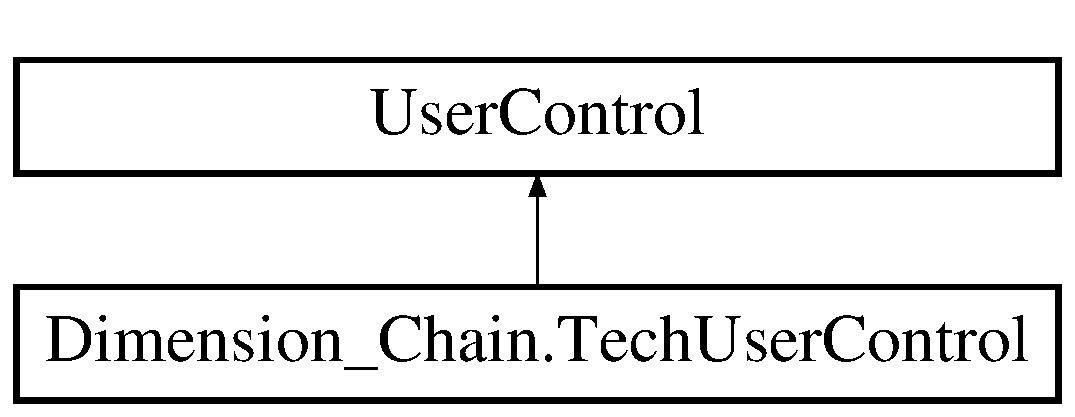
\includegraphics[height=2.000000cm]{class_dimension___chain_1_1_tech_user_control}
\end{center}
\end{figure}
\subsection*{Public Member Functions}
\begin{DoxyCompactItemize}
\item 
\mbox{\hyperlink{class_dimension___chain_1_1_tech_user_control_ae271e2a4e73a066d449e8653dbaf3ce1}{Tech\+User\+Control}} ()
\item 
void \mbox{\hyperlink{class_dimension___chain_1_1_tech_user_control_ae876b7a21937a3221ab9562fa5f30465}{Set\+U\+I\+\_\+\+TD}} (\mbox{\hyperlink{class_dimension___chain_1_1_u_i___tech_dimension}{U\+I\+\_\+\+Tech\+Dimension}} U\+I\+\_\+\+TD)
\item 
void \mbox{\hyperlink{class_dimension___chain_1_1_tech_user_control_a339e3419d46f0cda9188b3335ff57f4d}{Re\+Null}} ()
\end{DoxyCompactItemize}


\subsection{Detailed Description}
Логика взаимодействия для Dimension\+User\+Control.\+xaml 



\subsection{Constructor \& Destructor Documentation}
\mbox{\Hypertarget{class_dimension___chain_1_1_tech_user_control_ae271e2a4e73a066d449e8653dbaf3ce1}\label{class_dimension___chain_1_1_tech_user_control_ae271e2a4e73a066d449e8653dbaf3ce1}} 
\index{Dimension\+\_\+\+Chain\+::\+Tech\+User\+Control@{Dimension\+\_\+\+Chain\+::\+Tech\+User\+Control}!Tech\+User\+Control@{Tech\+User\+Control}}
\index{Tech\+User\+Control@{Tech\+User\+Control}!Dimension\+\_\+\+Chain\+::\+Tech\+User\+Control@{Dimension\+\_\+\+Chain\+::\+Tech\+User\+Control}}
\subsubsection{\texorpdfstring{Tech\+User\+Control()}{TechUserControl()}}
{\footnotesize\ttfamily Dimension\+\_\+\+Chain.\+Tech\+User\+Control.\+Tech\+User\+Control (\begin{DoxyParamCaption}{ }\end{DoxyParamCaption})}



\subsection{Member Function Documentation}
\mbox{\Hypertarget{class_dimension___chain_1_1_tech_user_control_a339e3419d46f0cda9188b3335ff57f4d}\label{class_dimension___chain_1_1_tech_user_control_a339e3419d46f0cda9188b3335ff57f4d}} 
\index{Dimension\+\_\+\+Chain\+::\+Tech\+User\+Control@{Dimension\+\_\+\+Chain\+::\+Tech\+User\+Control}!Re\+Null@{Re\+Null}}
\index{Re\+Null@{Re\+Null}!Dimension\+\_\+\+Chain\+::\+Tech\+User\+Control@{Dimension\+\_\+\+Chain\+::\+Tech\+User\+Control}}
\subsubsection{\texorpdfstring{Re\+Null()}{ReNull()}}
{\footnotesize\ttfamily void Dimension\+\_\+\+Chain.\+Tech\+User\+Control.\+Re\+Null (\begin{DoxyParamCaption}{ }\end{DoxyParamCaption})}

\mbox{\Hypertarget{class_dimension___chain_1_1_tech_user_control_ae876b7a21937a3221ab9562fa5f30465}\label{class_dimension___chain_1_1_tech_user_control_ae876b7a21937a3221ab9562fa5f30465}} 
\index{Dimension\+\_\+\+Chain\+::\+Tech\+User\+Control@{Dimension\+\_\+\+Chain\+::\+Tech\+User\+Control}!Set\+U\+I\+\_\+\+TD@{Set\+U\+I\+\_\+\+TD}}
\index{Set\+U\+I\+\_\+\+TD@{Set\+U\+I\+\_\+\+TD}!Dimension\+\_\+\+Chain\+::\+Tech\+User\+Control@{Dimension\+\_\+\+Chain\+::\+Tech\+User\+Control}}
\subsubsection{\texorpdfstring{Set\+U\+I\+\_\+\+T\+D()}{SetUI\_TD()}}
{\footnotesize\ttfamily void Dimension\+\_\+\+Chain.\+Tech\+User\+Control.\+Set\+U\+I\+\_\+\+TD (\begin{DoxyParamCaption}\item[{\mbox{\hyperlink{class_dimension___chain_1_1_u_i___tech_dimension}{U\+I\+\_\+\+Tech\+Dimension}}}]{U\+I\+\_\+\+TD }\end{DoxyParamCaption})}



The documentation for this class was generated from the following file\+:\begin{DoxyCompactItemize}
\item 
\mbox{\hyperlink{_tech_user_control_8xaml_8cs}{Tech\+User\+Control.\+xaml.\+cs}}\end{DoxyCompactItemize}

\hypertarget{class_dimension___chain_1_1_u_i___constr_dimension}{}\section{Dimension\+\_\+\+Chain.\+U\+I\+\_\+\+Constr\+Dimension Class Reference}
\label{class_dimension___chain_1_1_u_i___constr_dimension}\index{Dimension\+\_\+\+Chain.\+U\+I\+\_\+\+Constr\+Dimension@{Dimension\+\_\+\+Chain.\+U\+I\+\_\+\+Constr\+Dimension}}
Inheritance diagram for Dimension\+\_\+\+Chain.\+U\+I\+\_\+\+Constr\+Dimension\+:\begin{figure}[H]
\begin{center}
\leavevmode
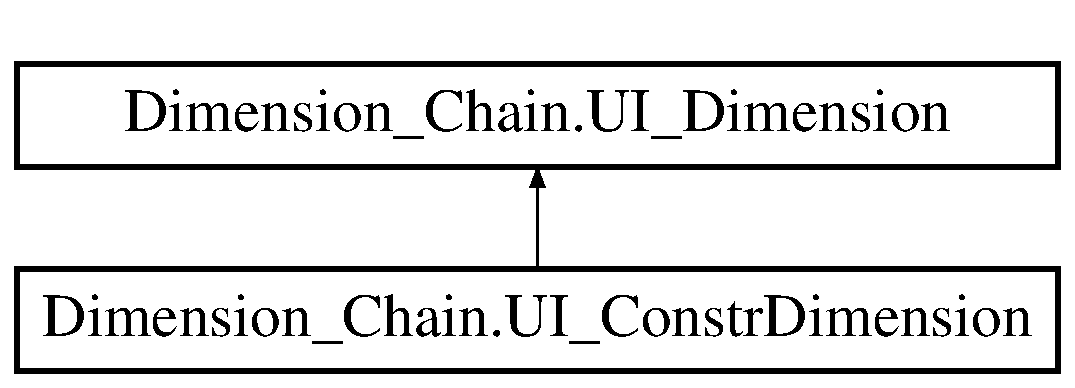
\includegraphics[height=2.000000cm]{class_dimension___chain_1_1_u_i___constr_dimension}
\end{center}
\end{figure}
\subsection*{Public Member Functions}
\begin{DoxyCompactItemize}
\item 
delegate void \mbox{\hyperlink{class_dimension___chain_1_1_u_i___constr_dimension_afb6b60fe4836094dcbf61d6347f94b24}{Constr\+Apdated\+Event\+Handler}} (\mbox{\hyperlink{class_dimension___chain_1_1_u_i___dimension}{U\+I\+\_\+\+Dimension}} dim)
\item 
\mbox{\hyperlink{class_dimension___chain_1_1_u_i___constr_dimension_a5a5a38f79b3822a6912010066cc1636b}{U\+I\+\_\+\+Constr\+Dimension}} (\mbox{\hyperlink{class_dimension___chain_1_1_constructor_user_control}{Constructor\+User\+Control}} C\+UC)
\item 
override void \mbox{\hyperlink{class_dimension___chain_1_1_u_i___constr_dimension_a9d4992d200a4fd5fde1b6dd6ccb03c91}{Set\+Other\+Labels}} ()
\item 
override void \mbox{\hyperlink{class_dimension___chain_1_1_u_i___constr_dimension_aacedc7ff420f11c4923787d58e116ef5}{lbl\+Clicked\+Other\+Podpiska}} ()
\item 
override void \mbox{\hyperlink{class_dimension___chain_1_1_u_i___constr_dimension_a3815be9b5b88d93c7912b14b4a61d587}{Otpiska\+When\+Delate}} ()
\item 
override void \mbox{\hyperlink{class_dimension___chain_1_1_u_i___constr_dimension_a376e3dccaacd2f13db6da8a7012ae0ad}{Remove\+Other\+Labels}} ()
\item 
override void \mbox{\hyperlink{class_dimension___chain_1_1_u_i___constr_dimension_ae763eed5acf7a38c8d7c6cb3734ffb16}{Not\+Alarm}} ()
\item 
void \mbox{\hyperlink{class_dimension___chain_1_1_u_i___constr_dimension_a8b994f742a4dca8a4accf2a3d3ebd809}{C\+U\+C\+\_\+\+Apdated}} ()
\item 
\mbox{\hyperlink{class_dimension___chain_1_1_u_i___constr_dimension_aed60aa3fee914ad924b29c5d65bcd463}{U\+I\+\_\+\+Constr\+Dimension}} (\mbox{\hyperlink{class_dimension___chain_1_1_u_i___dimension___save}{U\+I\+\_\+\+Dimension\+\_\+\+Save}} saved)
\end{DoxyCompactItemize}
\subsection*{Public Attributes}
\begin{DoxyCompactItemize}
\item 
double \mbox{\hyperlink{class_dimension___chain_1_1_u_i___constr_dimension_aa81df927b2b21106b0cbea8061a976be}{max}}
\item 
double \mbox{\hyperlink{class_dimension___chain_1_1_u_i___constr_dimension_aa4a7d8c97f9b60e388ff077bda093bae}{min}}
\item 
Label \mbox{\hyperlink{class_dimension___chain_1_1_u_i___constr_dimension_a565f224e437467d9575b55807b739d88}{lbl\+Nominal\+Constr}}
\item 
Label \mbox{\hyperlink{class_dimension___chain_1_1_u_i___constr_dimension_a09b6b3ccc0a3d464a5cafe34b38e9ab9}{lbl\+Up\+Constr}}
\item 
Label \mbox{\hyperlink{class_dimension___chain_1_1_u_i___constr_dimension_a3d01bbd22dcac507866e69d4c104318d}{lbl\+Down\+Constr}}
\end{DoxyCompactItemize}
\subsection*{Events}
\begin{DoxyCompactItemize}
\item 
\mbox{\hyperlink{class_dimension___chain_1_1_u_i___constr_dimension_afb6b60fe4836094dcbf61d6347f94b24}{Constr\+Apdated\+Event\+Handler}} \mbox{\hyperlink{class_dimension___chain_1_1_u_i___constr_dimension_aaf06553821087aeeddf8ac8c2e3b47ff}{Constr\+Apdated\+Event}}
\end{DoxyCompactItemize}
\subsection*{Additional Inherited Members}


\subsection{Constructor \& Destructor Documentation}
\mbox{\Hypertarget{class_dimension___chain_1_1_u_i___constr_dimension_a5a5a38f79b3822a6912010066cc1636b}\label{class_dimension___chain_1_1_u_i___constr_dimension_a5a5a38f79b3822a6912010066cc1636b}} 
\index{Dimension\+\_\+\+Chain\+::\+U\+I\+\_\+\+Constr\+Dimension@{Dimension\+\_\+\+Chain\+::\+U\+I\+\_\+\+Constr\+Dimension}!U\+I\+\_\+\+Constr\+Dimension@{U\+I\+\_\+\+Constr\+Dimension}}
\index{U\+I\+\_\+\+Constr\+Dimension@{U\+I\+\_\+\+Constr\+Dimension}!Dimension\+\_\+\+Chain\+::\+U\+I\+\_\+\+Constr\+Dimension@{Dimension\+\_\+\+Chain\+::\+U\+I\+\_\+\+Constr\+Dimension}}
\subsubsection{\texorpdfstring{U\+I\+\_\+\+Constr\+Dimension()}{UI\_ConstrDimension()}\hspace{0.1cm}{\footnotesize\ttfamily [1/2]}}
{\footnotesize\ttfamily Dimension\+\_\+\+Chain.\+U\+I\+\_\+\+Constr\+Dimension.\+U\+I\+\_\+\+Constr\+Dimension (\begin{DoxyParamCaption}\item[{\mbox{\hyperlink{class_dimension___chain_1_1_constructor_user_control}{Constructor\+User\+Control}}}]{C\+UC }\end{DoxyParamCaption})}

\mbox{\Hypertarget{class_dimension___chain_1_1_u_i___constr_dimension_aed60aa3fee914ad924b29c5d65bcd463}\label{class_dimension___chain_1_1_u_i___constr_dimension_aed60aa3fee914ad924b29c5d65bcd463}} 
\index{Dimension\+\_\+\+Chain\+::\+U\+I\+\_\+\+Constr\+Dimension@{Dimension\+\_\+\+Chain\+::\+U\+I\+\_\+\+Constr\+Dimension}!U\+I\+\_\+\+Constr\+Dimension@{U\+I\+\_\+\+Constr\+Dimension}}
\index{U\+I\+\_\+\+Constr\+Dimension@{U\+I\+\_\+\+Constr\+Dimension}!Dimension\+\_\+\+Chain\+::\+U\+I\+\_\+\+Constr\+Dimension@{Dimension\+\_\+\+Chain\+::\+U\+I\+\_\+\+Constr\+Dimension}}
\subsubsection{\texorpdfstring{U\+I\+\_\+\+Constr\+Dimension()}{UI\_ConstrDimension()}\hspace{0.1cm}{\footnotesize\ttfamily [2/2]}}
{\footnotesize\ttfamily Dimension\+\_\+\+Chain.\+U\+I\+\_\+\+Constr\+Dimension.\+U\+I\+\_\+\+Constr\+Dimension (\begin{DoxyParamCaption}\item[{\mbox{\hyperlink{class_dimension___chain_1_1_u_i___dimension___save}{U\+I\+\_\+\+Dimension\+\_\+\+Save}}}]{saved }\end{DoxyParamCaption})}



\subsection{Member Function Documentation}
\mbox{\Hypertarget{class_dimension___chain_1_1_u_i___constr_dimension_afb6b60fe4836094dcbf61d6347f94b24}\label{class_dimension___chain_1_1_u_i___constr_dimension_afb6b60fe4836094dcbf61d6347f94b24}} 
\index{Dimension\+\_\+\+Chain\+::\+U\+I\+\_\+\+Constr\+Dimension@{Dimension\+\_\+\+Chain\+::\+U\+I\+\_\+\+Constr\+Dimension}!Constr\+Apdated\+Event\+Handler@{Constr\+Apdated\+Event\+Handler}}
\index{Constr\+Apdated\+Event\+Handler@{Constr\+Apdated\+Event\+Handler}!Dimension\+\_\+\+Chain\+::\+U\+I\+\_\+\+Constr\+Dimension@{Dimension\+\_\+\+Chain\+::\+U\+I\+\_\+\+Constr\+Dimension}}
\subsubsection{\texorpdfstring{Constr\+Apdated\+Event\+Handler()}{ConstrApdatedEventHandler()}}
{\footnotesize\ttfamily delegate void Dimension\+\_\+\+Chain.\+U\+I\+\_\+\+Constr\+Dimension.\+Constr\+Apdated\+Event\+Handler (\begin{DoxyParamCaption}\item[{\mbox{\hyperlink{class_dimension___chain_1_1_u_i___dimension}{U\+I\+\_\+\+Dimension}}}]{dim }\end{DoxyParamCaption})}

\mbox{\Hypertarget{class_dimension___chain_1_1_u_i___constr_dimension_a8b994f742a4dca8a4accf2a3d3ebd809}\label{class_dimension___chain_1_1_u_i___constr_dimension_a8b994f742a4dca8a4accf2a3d3ebd809}} 
\index{Dimension\+\_\+\+Chain\+::\+U\+I\+\_\+\+Constr\+Dimension@{Dimension\+\_\+\+Chain\+::\+U\+I\+\_\+\+Constr\+Dimension}!C\+U\+C\+\_\+\+Apdated@{C\+U\+C\+\_\+\+Apdated}}
\index{C\+U\+C\+\_\+\+Apdated@{C\+U\+C\+\_\+\+Apdated}!Dimension\+\_\+\+Chain\+::\+U\+I\+\_\+\+Constr\+Dimension@{Dimension\+\_\+\+Chain\+::\+U\+I\+\_\+\+Constr\+Dimension}}
\subsubsection{\texorpdfstring{C\+U\+C\+\_\+\+Apdated()}{CUC\_Apdated()}}
{\footnotesize\ttfamily void Dimension\+\_\+\+Chain.\+U\+I\+\_\+\+Constr\+Dimension.\+C\+U\+C\+\_\+\+Apdated (\begin{DoxyParamCaption}{ }\end{DoxyParamCaption})}

\mbox{\Hypertarget{class_dimension___chain_1_1_u_i___constr_dimension_aacedc7ff420f11c4923787d58e116ef5}\label{class_dimension___chain_1_1_u_i___constr_dimension_aacedc7ff420f11c4923787d58e116ef5}} 
\index{Dimension\+\_\+\+Chain\+::\+U\+I\+\_\+\+Constr\+Dimension@{Dimension\+\_\+\+Chain\+::\+U\+I\+\_\+\+Constr\+Dimension}!lbl\+Clicked\+Other\+Podpiska@{lbl\+Clicked\+Other\+Podpiska}}
\index{lbl\+Clicked\+Other\+Podpiska@{lbl\+Clicked\+Other\+Podpiska}!Dimension\+\_\+\+Chain\+::\+U\+I\+\_\+\+Constr\+Dimension@{Dimension\+\_\+\+Chain\+::\+U\+I\+\_\+\+Constr\+Dimension}}
\subsubsection{\texorpdfstring{lbl\+Clicked\+Other\+Podpiska()}{lblClickedOtherPodpiska()}}
{\footnotesize\ttfamily override void Dimension\+\_\+\+Chain.\+U\+I\+\_\+\+Constr\+Dimension.\+lbl\+Clicked\+Other\+Podpiska (\begin{DoxyParamCaption}{ }\end{DoxyParamCaption})\hspace{0.3cm}{\ttfamily [virtual]}}



Reimplemented from \mbox{\hyperlink{class_dimension___chain_1_1_u_i___dimension_a13210c593c5bd0f5e7b59b93f6ec5fdc}{Dimension\+\_\+\+Chain.\+U\+I\+\_\+\+Dimension}}.

\mbox{\Hypertarget{class_dimension___chain_1_1_u_i___constr_dimension_ae763eed5acf7a38c8d7c6cb3734ffb16}\label{class_dimension___chain_1_1_u_i___constr_dimension_ae763eed5acf7a38c8d7c6cb3734ffb16}} 
\index{Dimension\+\_\+\+Chain\+::\+U\+I\+\_\+\+Constr\+Dimension@{Dimension\+\_\+\+Chain\+::\+U\+I\+\_\+\+Constr\+Dimension}!Not\+Alarm@{Not\+Alarm}}
\index{Not\+Alarm@{Not\+Alarm}!Dimension\+\_\+\+Chain\+::\+U\+I\+\_\+\+Constr\+Dimension@{Dimension\+\_\+\+Chain\+::\+U\+I\+\_\+\+Constr\+Dimension}}
\subsubsection{\texorpdfstring{Not\+Alarm()}{NotAlarm()}}
{\footnotesize\ttfamily override void Dimension\+\_\+\+Chain.\+U\+I\+\_\+\+Constr\+Dimension.\+Not\+Alarm (\begin{DoxyParamCaption}{ }\end{DoxyParamCaption})\hspace{0.3cm}{\ttfamily [virtual]}}



Reimplemented from \mbox{\hyperlink{class_dimension___chain_1_1_u_i___dimension_a4ab4c36c068571222229db5f0a194dd2}{Dimension\+\_\+\+Chain.\+U\+I\+\_\+\+Dimension}}.

\mbox{\Hypertarget{class_dimension___chain_1_1_u_i___constr_dimension_a3815be9b5b88d93c7912b14b4a61d587}\label{class_dimension___chain_1_1_u_i___constr_dimension_a3815be9b5b88d93c7912b14b4a61d587}} 
\index{Dimension\+\_\+\+Chain\+::\+U\+I\+\_\+\+Constr\+Dimension@{Dimension\+\_\+\+Chain\+::\+U\+I\+\_\+\+Constr\+Dimension}!Otpiska\+When\+Delate@{Otpiska\+When\+Delate}}
\index{Otpiska\+When\+Delate@{Otpiska\+When\+Delate}!Dimension\+\_\+\+Chain\+::\+U\+I\+\_\+\+Constr\+Dimension@{Dimension\+\_\+\+Chain\+::\+U\+I\+\_\+\+Constr\+Dimension}}
\subsubsection{\texorpdfstring{Otpiska\+When\+Delate()}{OtpiskaWhenDelate()}}
{\footnotesize\ttfamily override void Dimension\+\_\+\+Chain.\+U\+I\+\_\+\+Constr\+Dimension.\+Otpiska\+When\+Delate (\begin{DoxyParamCaption}{ }\end{DoxyParamCaption})\hspace{0.3cm}{\ttfamily [virtual]}}



Reimplemented from \mbox{\hyperlink{class_dimension___chain_1_1_u_i___dimension_aad38da2794443edfca137c15e417bfd3}{Dimension\+\_\+\+Chain.\+U\+I\+\_\+\+Dimension}}.

\mbox{\Hypertarget{class_dimension___chain_1_1_u_i___constr_dimension_a376e3dccaacd2f13db6da8a7012ae0ad}\label{class_dimension___chain_1_1_u_i___constr_dimension_a376e3dccaacd2f13db6da8a7012ae0ad}} 
\index{Dimension\+\_\+\+Chain\+::\+U\+I\+\_\+\+Constr\+Dimension@{Dimension\+\_\+\+Chain\+::\+U\+I\+\_\+\+Constr\+Dimension}!Remove\+Other\+Labels@{Remove\+Other\+Labels}}
\index{Remove\+Other\+Labels@{Remove\+Other\+Labels}!Dimension\+\_\+\+Chain\+::\+U\+I\+\_\+\+Constr\+Dimension@{Dimension\+\_\+\+Chain\+::\+U\+I\+\_\+\+Constr\+Dimension}}
\subsubsection{\texorpdfstring{Remove\+Other\+Labels()}{RemoveOtherLabels()}}
{\footnotesize\ttfamily override void Dimension\+\_\+\+Chain.\+U\+I\+\_\+\+Constr\+Dimension.\+Remove\+Other\+Labels (\begin{DoxyParamCaption}{ }\end{DoxyParamCaption})\hspace{0.3cm}{\ttfamily [virtual]}}



Reimplemented from \mbox{\hyperlink{class_dimension___chain_1_1_u_i___dimension_a17854a85eba47798b7459b633f1db4bb}{Dimension\+\_\+\+Chain.\+U\+I\+\_\+\+Dimension}}.

\mbox{\Hypertarget{class_dimension___chain_1_1_u_i___constr_dimension_a9d4992d200a4fd5fde1b6dd6ccb03c91}\label{class_dimension___chain_1_1_u_i___constr_dimension_a9d4992d200a4fd5fde1b6dd6ccb03c91}} 
\index{Dimension\+\_\+\+Chain\+::\+U\+I\+\_\+\+Constr\+Dimension@{Dimension\+\_\+\+Chain\+::\+U\+I\+\_\+\+Constr\+Dimension}!Set\+Other\+Labels@{Set\+Other\+Labels}}
\index{Set\+Other\+Labels@{Set\+Other\+Labels}!Dimension\+\_\+\+Chain\+::\+U\+I\+\_\+\+Constr\+Dimension@{Dimension\+\_\+\+Chain\+::\+U\+I\+\_\+\+Constr\+Dimension}}
\subsubsection{\texorpdfstring{Set\+Other\+Labels()}{SetOtherLabels()}}
{\footnotesize\ttfamily override void Dimension\+\_\+\+Chain.\+U\+I\+\_\+\+Constr\+Dimension.\+Set\+Other\+Labels (\begin{DoxyParamCaption}{ }\end{DoxyParamCaption})\hspace{0.3cm}{\ttfamily [virtual]}}



Reimplemented from \mbox{\hyperlink{class_dimension___chain_1_1_u_i___dimension_a78774f971a6494a57310623f4bf0aa4f}{Dimension\+\_\+\+Chain.\+U\+I\+\_\+\+Dimension}}.



\subsection{Member Data Documentation}
\mbox{\Hypertarget{class_dimension___chain_1_1_u_i___constr_dimension_a3d01bbd22dcac507866e69d4c104318d}\label{class_dimension___chain_1_1_u_i___constr_dimension_a3d01bbd22dcac507866e69d4c104318d}} 
\index{Dimension\+\_\+\+Chain\+::\+U\+I\+\_\+\+Constr\+Dimension@{Dimension\+\_\+\+Chain\+::\+U\+I\+\_\+\+Constr\+Dimension}!lbl\+Down\+Constr@{lbl\+Down\+Constr}}
\index{lbl\+Down\+Constr@{lbl\+Down\+Constr}!Dimension\+\_\+\+Chain\+::\+U\+I\+\_\+\+Constr\+Dimension@{Dimension\+\_\+\+Chain\+::\+U\+I\+\_\+\+Constr\+Dimension}}
\subsubsection{\texorpdfstring{lbl\+Down\+Constr}{lblDownConstr}}
{\footnotesize\ttfamily Label Dimension\+\_\+\+Chain.\+U\+I\+\_\+\+Constr\+Dimension.\+lbl\+Down\+Constr}

\mbox{\Hypertarget{class_dimension___chain_1_1_u_i___constr_dimension_a565f224e437467d9575b55807b739d88}\label{class_dimension___chain_1_1_u_i___constr_dimension_a565f224e437467d9575b55807b739d88}} 
\index{Dimension\+\_\+\+Chain\+::\+U\+I\+\_\+\+Constr\+Dimension@{Dimension\+\_\+\+Chain\+::\+U\+I\+\_\+\+Constr\+Dimension}!lbl\+Nominal\+Constr@{lbl\+Nominal\+Constr}}
\index{lbl\+Nominal\+Constr@{lbl\+Nominal\+Constr}!Dimension\+\_\+\+Chain\+::\+U\+I\+\_\+\+Constr\+Dimension@{Dimension\+\_\+\+Chain\+::\+U\+I\+\_\+\+Constr\+Dimension}}
\subsubsection{\texorpdfstring{lbl\+Nominal\+Constr}{lblNominalConstr}}
{\footnotesize\ttfamily Label Dimension\+\_\+\+Chain.\+U\+I\+\_\+\+Constr\+Dimension.\+lbl\+Nominal\+Constr}

\mbox{\Hypertarget{class_dimension___chain_1_1_u_i___constr_dimension_a09b6b3ccc0a3d464a5cafe34b38e9ab9}\label{class_dimension___chain_1_1_u_i___constr_dimension_a09b6b3ccc0a3d464a5cafe34b38e9ab9}} 
\index{Dimension\+\_\+\+Chain\+::\+U\+I\+\_\+\+Constr\+Dimension@{Dimension\+\_\+\+Chain\+::\+U\+I\+\_\+\+Constr\+Dimension}!lbl\+Up\+Constr@{lbl\+Up\+Constr}}
\index{lbl\+Up\+Constr@{lbl\+Up\+Constr}!Dimension\+\_\+\+Chain\+::\+U\+I\+\_\+\+Constr\+Dimension@{Dimension\+\_\+\+Chain\+::\+U\+I\+\_\+\+Constr\+Dimension}}
\subsubsection{\texorpdfstring{lbl\+Up\+Constr}{lblUpConstr}}
{\footnotesize\ttfamily Label Dimension\+\_\+\+Chain.\+U\+I\+\_\+\+Constr\+Dimension.\+lbl\+Up\+Constr}

\mbox{\Hypertarget{class_dimension___chain_1_1_u_i___constr_dimension_aa81df927b2b21106b0cbea8061a976be}\label{class_dimension___chain_1_1_u_i___constr_dimension_aa81df927b2b21106b0cbea8061a976be}} 
\index{Dimension\+\_\+\+Chain\+::\+U\+I\+\_\+\+Constr\+Dimension@{Dimension\+\_\+\+Chain\+::\+U\+I\+\_\+\+Constr\+Dimension}!max@{max}}
\index{max@{max}!Dimension\+\_\+\+Chain\+::\+U\+I\+\_\+\+Constr\+Dimension@{Dimension\+\_\+\+Chain\+::\+U\+I\+\_\+\+Constr\+Dimension}}
\subsubsection{\texorpdfstring{max}{max}}
{\footnotesize\ttfamily double Dimension\+\_\+\+Chain.\+U\+I\+\_\+\+Constr\+Dimension.\+max}

\mbox{\Hypertarget{class_dimension___chain_1_1_u_i___constr_dimension_aa4a7d8c97f9b60e388ff077bda093bae}\label{class_dimension___chain_1_1_u_i___constr_dimension_aa4a7d8c97f9b60e388ff077bda093bae}} 
\index{Dimension\+\_\+\+Chain\+::\+U\+I\+\_\+\+Constr\+Dimension@{Dimension\+\_\+\+Chain\+::\+U\+I\+\_\+\+Constr\+Dimension}!min@{min}}
\index{min@{min}!Dimension\+\_\+\+Chain\+::\+U\+I\+\_\+\+Constr\+Dimension@{Dimension\+\_\+\+Chain\+::\+U\+I\+\_\+\+Constr\+Dimension}}
\subsubsection{\texorpdfstring{min}{min}}
{\footnotesize\ttfamily double Dimension\+\_\+\+Chain.\+U\+I\+\_\+\+Constr\+Dimension.\+min}



\subsection{Event Documentation}
\mbox{\Hypertarget{class_dimension___chain_1_1_u_i___constr_dimension_aaf06553821087aeeddf8ac8c2e3b47ff}\label{class_dimension___chain_1_1_u_i___constr_dimension_aaf06553821087aeeddf8ac8c2e3b47ff}} 
\index{Dimension\+\_\+\+Chain\+::\+U\+I\+\_\+\+Constr\+Dimension@{Dimension\+\_\+\+Chain\+::\+U\+I\+\_\+\+Constr\+Dimension}!Constr\+Apdated\+Event@{Constr\+Apdated\+Event}}
\index{Constr\+Apdated\+Event@{Constr\+Apdated\+Event}!Dimension\+\_\+\+Chain\+::\+U\+I\+\_\+\+Constr\+Dimension@{Dimension\+\_\+\+Chain\+::\+U\+I\+\_\+\+Constr\+Dimension}}
\subsubsection{\texorpdfstring{Constr\+Apdated\+Event}{ConstrApdatedEvent}}
{\footnotesize\ttfamily \mbox{\hyperlink{class_dimension___chain_1_1_u_i___constr_dimension_afb6b60fe4836094dcbf61d6347f94b24}{Constr\+Apdated\+Event\+Handler}} Dimension\+\_\+\+Chain.\+U\+I\+\_\+\+Constr\+Dimension.\+Constr\+Apdated\+Event}



The documentation for this class was generated from the following files\+:\begin{DoxyCompactItemize}
\item 
\mbox{\hyperlink{_u_i___constr_dimension_8cs}{U\+I\+\_\+\+Constr\+Dimension.\+cs}}\item 
\mbox{\hyperlink{_u_i___dimension_partial_8cs}{U\+I\+\_\+\+Dimension\+Partial.\+cs}}\end{DoxyCompactItemize}

\hypertarget{class_dimension___chain_1_1_u_i___constr_dimension___save}{}\section{Dimension\+\_\+\+Chain.\+U\+I\+\_\+\+Constr\+Dimension\+\_\+\+Save Class Reference}
\label{class_dimension___chain_1_1_u_i___constr_dimension___save}\index{Dimension\+\_\+\+Chain.\+U\+I\+\_\+\+Constr\+Dimension\+\_\+\+Save@{Dimension\+\_\+\+Chain.\+U\+I\+\_\+\+Constr\+Dimension\+\_\+\+Save}}
Inheritance diagram for Dimension\+\_\+\+Chain.\+U\+I\+\_\+\+Constr\+Dimension\+\_\+\+Save\+:\begin{figure}[H]
\begin{center}
\leavevmode
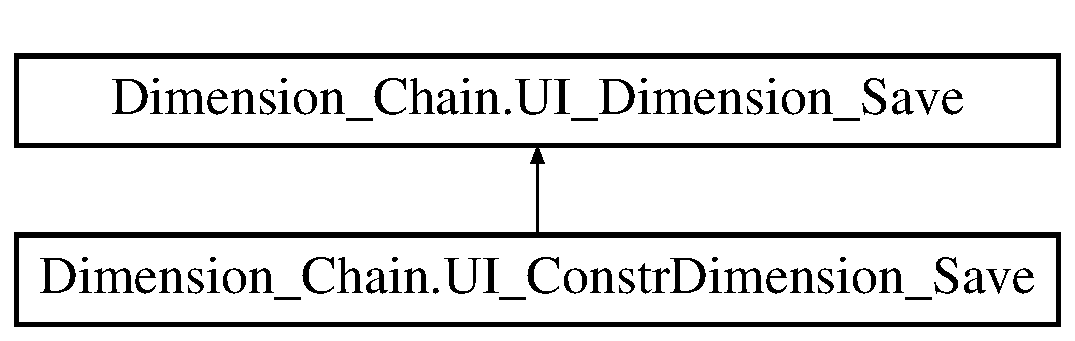
\includegraphics[height=2.000000cm]{class_dimension___chain_1_1_u_i___constr_dimension___save}
\end{center}
\end{figure}
\subsection*{Public Member Functions}
\begin{DoxyCompactItemize}
\item 
\mbox{\hyperlink{class_dimension___chain_1_1_u_i___constr_dimension___save_a1c070c16eea1a24236aaf69e42bc5294}{U\+I\+\_\+\+Constr\+Dimension\+\_\+\+Save}} (\mbox{\hyperlink{class_dimension___chain_1_1_u_i___constr_dimension}{U\+I\+\_\+\+Constr\+Dimension}} dim)
\end{DoxyCompactItemize}
\subsection*{Public Attributes}
\begin{DoxyCompactItemize}
\item 
double \mbox{\hyperlink{class_dimension___chain_1_1_u_i___constr_dimension___save_a98e59e579076a0ac37836f972cedf3e2}{nominal}}
\item 
double \mbox{\hyperlink{class_dimension___chain_1_1_u_i___constr_dimension___save_aeba39bf37b5a6bdfc172e4597e1a868c}{up}}
\item 
double \mbox{\hyperlink{class_dimension___chain_1_1_u_i___constr_dimension___save_a616826bce06d95345b5e3bf096728cf3}{down}}
\end{DoxyCompactItemize}


\subsection{Constructor \& Destructor Documentation}
\mbox{\Hypertarget{class_dimension___chain_1_1_u_i___constr_dimension___save_a1c070c16eea1a24236aaf69e42bc5294}\label{class_dimension___chain_1_1_u_i___constr_dimension___save_a1c070c16eea1a24236aaf69e42bc5294}} 
\index{Dimension\+\_\+\+Chain\+::\+U\+I\+\_\+\+Constr\+Dimension\+\_\+\+Save@{Dimension\+\_\+\+Chain\+::\+U\+I\+\_\+\+Constr\+Dimension\+\_\+\+Save}!U\+I\+\_\+\+Constr\+Dimension\+\_\+\+Save@{U\+I\+\_\+\+Constr\+Dimension\+\_\+\+Save}}
\index{U\+I\+\_\+\+Constr\+Dimension\+\_\+\+Save@{U\+I\+\_\+\+Constr\+Dimension\+\_\+\+Save}!Dimension\+\_\+\+Chain\+::\+U\+I\+\_\+\+Constr\+Dimension\+\_\+\+Save@{Dimension\+\_\+\+Chain\+::\+U\+I\+\_\+\+Constr\+Dimension\+\_\+\+Save}}
\subsubsection{\texorpdfstring{U\+I\+\_\+\+Constr\+Dimension\+\_\+\+Save()}{UI\_ConstrDimension\_Save()}}
{\footnotesize\ttfamily Dimension\+\_\+\+Chain.\+U\+I\+\_\+\+Constr\+Dimension\+\_\+\+Save.\+U\+I\+\_\+\+Constr\+Dimension\+\_\+\+Save (\begin{DoxyParamCaption}\item[{\mbox{\hyperlink{class_dimension___chain_1_1_u_i___constr_dimension}{U\+I\+\_\+\+Constr\+Dimension}}}]{dim }\end{DoxyParamCaption})}



\subsection{Member Data Documentation}
\mbox{\Hypertarget{class_dimension___chain_1_1_u_i___constr_dimension___save_a616826bce06d95345b5e3bf096728cf3}\label{class_dimension___chain_1_1_u_i___constr_dimension___save_a616826bce06d95345b5e3bf096728cf3}} 
\index{Dimension\+\_\+\+Chain\+::\+U\+I\+\_\+\+Constr\+Dimension\+\_\+\+Save@{Dimension\+\_\+\+Chain\+::\+U\+I\+\_\+\+Constr\+Dimension\+\_\+\+Save}!down@{down}}
\index{down@{down}!Dimension\+\_\+\+Chain\+::\+U\+I\+\_\+\+Constr\+Dimension\+\_\+\+Save@{Dimension\+\_\+\+Chain\+::\+U\+I\+\_\+\+Constr\+Dimension\+\_\+\+Save}}
\subsubsection{\texorpdfstring{down}{down}}
{\footnotesize\ttfamily double Dimension\+\_\+\+Chain.\+U\+I\+\_\+\+Constr\+Dimension\+\_\+\+Save.\+down}

\mbox{\Hypertarget{class_dimension___chain_1_1_u_i___constr_dimension___save_a98e59e579076a0ac37836f972cedf3e2}\label{class_dimension___chain_1_1_u_i___constr_dimension___save_a98e59e579076a0ac37836f972cedf3e2}} 
\index{Dimension\+\_\+\+Chain\+::\+U\+I\+\_\+\+Constr\+Dimension\+\_\+\+Save@{Dimension\+\_\+\+Chain\+::\+U\+I\+\_\+\+Constr\+Dimension\+\_\+\+Save}!nominal@{nominal}}
\index{nominal@{nominal}!Dimension\+\_\+\+Chain\+::\+U\+I\+\_\+\+Constr\+Dimension\+\_\+\+Save@{Dimension\+\_\+\+Chain\+::\+U\+I\+\_\+\+Constr\+Dimension\+\_\+\+Save}}
\subsubsection{\texorpdfstring{nominal}{nominal}}
{\footnotesize\ttfamily double Dimension\+\_\+\+Chain.\+U\+I\+\_\+\+Constr\+Dimension\+\_\+\+Save.\+nominal}

\mbox{\Hypertarget{class_dimension___chain_1_1_u_i___constr_dimension___save_aeba39bf37b5a6bdfc172e4597e1a868c}\label{class_dimension___chain_1_1_u_i___constr_dimension___save_aeba39bf37b5a6bdfc172e4597e1a868c}} 
\index{Dimension\+\_\+\+Chain\+::\+U\+I\+\_\+\+Constr\+Dimension\+\_\+\+Save@{Dimension\+\_\+\+Chain\+::\+U\+I\+\_\+\+Constr\+Dimension\+\_\+\+Save}!up@{up}}
\index{up@{up}!Dimension\+\_\+\+Chain\+::\+U\+I\+\_\+\+Constr\+Dimension\+\_\+\+Save@{Dimension\+\_\+\+Chain\+::\+U\+I\+\_\+\+Constr\+Dimension\+\_\+\+Save}}
\subsubsection{\texorpdfstring{up}{up}}
{\footnotesize\ttfamily double Dimension\+\_\+\+Chain.\+U\+I\+\_\+\+Constr\+Dimension\+\_\+\+Save.\+up}



The documentation for this class was generated from the following file\+:\begin{DoxyCompactItemize}
\item 
\mbox{\hyperlink{_save_8cs}{Save.\+cs}}\end{DoxyCompactItemize}

\hypertarget{class_dimension___chain_1_1_u_i___dimension}{}\section{Dimension\+\_\+\+Chain.\+U\+I\+\_\+\+Dimension Class Reference}
\label{class_dimension___chain_1_1_u_i___dimension}\index{Dimension\+\_\+\+Chain.\+U\+I\+\_\+\+Dimension@{Dimension\+\_\+\+Chain.\+U\+I\+\_\+\+Dimension}}
Inheritance diagram for Dimension\+\_\+\+Chain.\+U\+I\+\_\+\+Dimension\+:\begin{figure}[H]
\begin{center}
\leavevmode
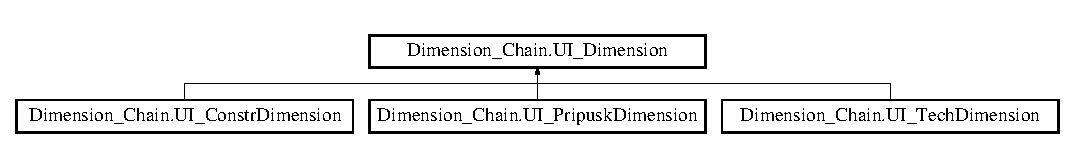
\includegraphics[height=1.555556cm]{class_dimension___chain_1_1_u_i___dimension}
\end{center}
\end{figure}
\subsection*{Public Member Functions}
\begin{DoxyCompactItemize}
\item 
delegate void \mbox{\hyperlink{class_dimension___chain_1_1_u_i___dimension_a106096e0c35875f5fab0e7f22e0b5941}{Dimension\+Created\+Event\+Handler}} (\mbox{\hyperlink{class_dimension___chain_1_1_u_i___dimension}{U\+I\+\_\+\+Dimension}} dim)
\item 
delegate void \mbox{\hyperlink{class_dimension___chain_1_1_u_i___dimension_a45fef985621de3e250d8343eeeca3aed}{dimension\+Clicked\+Event\+Handler}} (\mbox{\hyperlink{class_dimension___chain_1_1_u_i___dimension}{U\+I\+\_\+\+Dimension}} dim)
\item 
virtual User\+Control \mbox{\hyperlink{class_dimension___chain_1_1_u_i___dimension_a7aff55d45ac01c21db9f45583fe5c51c}{Create\+User\+Control}} ()
\item 
void \mbox{\hyperlink{class_dimension___chain_1_1_u_i___dimension_a3e4e1d9c20e13324015ff92665916cd1}{Set\+Nominal}} (string s)
\item 
void \mbox{\hyperlink{class_dimension___chain_1_1_u_i___dimension_a085021a542b0342c1acb0b0f147f1d1a}{Set\+Up}} (string s)
\item 
void \mbox{\hyperlink{class_dimension___chain_1_1_u_i___dimension_a95aaf2a3e9eebd27a6de7c4c2613c362}{Set\+Down}} (string s)
\item 
virtual void \mbox{\hyperlink{class_dimension___chain_1_1_u_i___dimension_a13210c593c5bd0f5e7b59b93f6ec5fdc}{lbl\+Clicked\+Other\+Podpiska}} ()
\item 
void \mbox{\hyperlink{class_dimension___chain_1_1_u_i___dimension_ac655b429f2293b499eb3c597ebd74b95}{Pick}} ()
\item 
void \mbox{\hyperlink{class_dimension___chain_1_1_u_i___dimension_a8d3d92dd9e720171068d5c92220c5669}{Unpick}} ()
\item 
void \mbox{\hyperlink{class_dimension___chain_1_1_u_i___dimension_a3dc1cd92d14d6df43a6a15dd739aa155}{Alarm}} ()
\item 
virtual void \mbox{\hyperlink{class_dimension___chain_1_1_u_i___dimension_a4ab4c36c068571222229db5f0a194dd2}{Not\+Alarm}} ()
\item 
void \mbox{\hyperlink{class_dimension___chain_1_1_u_i___dimension_ae3e15f8c2a0c7b66f6346438a3eae72a}{Remove\+From\+Canv}} ()
\item 
virtual void \mbox{\hyperlink{class_dimension___chain_1_1_u_i___dimension_a17854a85eba47798b7459b633f1db4bb}{Remove\+Other\+Labels}} ()
\item 
void \mbox{\hyperlink{class_dimension___chain_1_1_u_i___dimension_a1973f56d9bd88725bf942bedd6d8d98d}{Otpiska\+When\+Create}} ()
\item 
virtual void \mbox{\hyperlink{class_dimension___chain_1_1_u_i___dimension_aad38da2794443edfca137c15e417bfd3}{Otpiska\+When\+Delate}} ()
\item 
virtual void \mbox{\hyperlink{class_dimension___chain_1_1_u_i___dimension_a78774f971a6494a57310623f4bf0aa4f}{Set\+Other\+Labels}} ()
\item 
virtual void \mbox{\hyperlink{class_dimension___chain_1_1_u_i___dimension_a93110c560bdd2e03e4a943be85a0f913}{Unchoose}} ()
\item 
void \mbox{\hyperlink{class_dimension___chain_1_1_u_i___dimension_a91003f2c8039c015960f15fddc418d40}{Set\+Up\+Down\+Lbls}} ()
\item 
void \mbox{\hyperlink{class_dimension___chain_1_1_u_i___dimension_a708fa8978d862ed4be1507422b99c772}{Rebuild\+After\+Scale}} ()
\item 
\mbox{\hyperlink{class_dimension___chain_1_1_u_i___dimension_a75cba81921c322680810bd593d515958}{U\+I\+\_\+\+Dimension}} (\mbox{\hyperlink{class_dimension___chain_1_1_u_i___dimension___save}{U\+I\+\_\+\+Dimension\+\_\+\+Save}} saved)
\end{DoxyCompactItemize}
\subsection*{Public Attributes}
\begin{DoxyCompactItemize}
\item 
User\+Control \mbox{\hyperlink{class_dimension___chain_1_1_u_i___dimension_ade41252d28cea667eee14bad5bc1f9a2}{UC}}
\item 
\mbox{\hyperlink{namespace_dimension___chain_a6ec9051138598c61cc00acf2547dced4}{type}} \mbox{\hyperlink{class_dimension___chain_1_1_u_i___dimension_a6b40d21e1d4e51662827a615ef8f7564}{tp}}
\item 
double \mbox{\hyperlink{class_dimension___chain_1_1_u_i___dimension_aacc27fe94a037362f35b1c697cc671b4}{nominal}}
\item 
double \mbox{\hyperlink{class_dimension___chain_1_1_u_i___dimension_a3707451432d8b5471987be754732a75d}{up}}
\item 
double \mbox{\hyperlink{class_dimension___chain_1_1_u_i___dimension_a9893562e547e690ab725abce322a6a93}{down}}
\item 
Line \mbox{\hyperlink{class_dimension___chain_1_1_u_i___dimension_a73fe19b1c68179a37404e48d507b3901}{main\+Line}}
\item 
Label \mbox{\hyperlink{class_dimension___chain_1_1_u_i___dimension_ae78dcce1629029eade09cb44f4a97fa1}{lbl\+Nominal}}
\item 
Label \mbox{\hyperlink{class_dimension___chain_1_1_u_i___dimension_a799c81f3afaccb4e41fb19f099115108}{lbl\+Up}}
\item 
Label \mbox{\hyperlink{class_dimension___chain_1_1_u_i___dimension_a846b7751f2e526b7e30d0adffeac2327}{lbl\+Down}}
\item 
double \mbox{\hyperlink{class_dimension___chain_1_1_u_i___dimension_ab318784d1335aab7dd2622dbe7b28581}{first\+ElX}}
\item 
double \mbox{\hyperlink{class_dimension___chain_1_1_u_i___dimension_a37095262fa1ad821965fffb198842a3b}{first\+ElY}}
\item 
double \mbox{\hyperlink{class_dimension___chain_1_1_u_i___dimension_a134bfa41b935cd3250fc11cd5c1162e0}{second\+ElX}}
\item 
double \mbox{\hyperlink{class_dimension___chain_1_1_u_i___dimension_a55a719dbec616ef27aa758244c9eed64}{second\+ElY}}
\end{DoxyCompactItemize}
\subsection*{Static Public Attributes}
\begin{DoxyCompactItemize}
\item 
static Canvas \mbox{\hyperlink{class_dimension___chain_1_1_u_i___dimension_ab1481e824605880527852c9c0827f1cd}{canv}}
\item 
static Stack\+Panel \mbox{\hyperlink{class_dimension___chain_1_1_u_i___dimension_a4285006e5a9e3ce55d81cd1d4cb56845}{stack\+Panel}}
\item 
static List$<$ \mbox{\hyperlink{class_dimension___chain_1_1_u_i___dimension}{U\+I\+\_\+\+Dimension}} $>$ \mbox{\hyperlink{class_dimension___chain_1_1_u_i___dimension_a4186c0c50764c0bd5d6984cce1591777}{list\+Of\+Dimensions}}
\item 
static \mbox{\hyperlink{class_dimension___chain_1_1_u_i___dimension}{U\+I\+\_\+\+Dimension}} \mbox{\hyperlink{class_dimension___chain_1_1_u_i___dimension_aa5261f63d4d25236736bb1bb5236da25}{temporary\+UI}}
\end{DoxyCompactItemize}
\subsection*{Protected Member Functions}
\begin{DoxyCompactItemize}
\item 
\mbox{\hyperlink{class_dimension___chain_1_1_u_i___dimension_acd224ad860f38ed89790f0e9aa1321d6}{U\+I\+\_\+\+Dimension}} (User\+Control \mbox{\hyperlink{class_dimension___chain_1_1_u_i___dimension_ade41252d28cea667eee14bad5bc1f9a2}{UC}})
\item 
void \mbox{\hyperlink{class_dimension___chain_1_1_u_i___dimension_af9e7104a0bc09e67b0e3813ee8304ca1}{Create\+Basic\+Fields}} ()
\item 
void \mbox{\hyperlink{class_dimension___chain_1_1_u_i___dimension_aec30a2016b40e83553447c125d08fb68}{canv\+\_\+\+Mouse\+Left\+Button\+Down\+First\+Ellipse}} (object sender, Mouse\+Button\+Event\+Args e)
\item 
void \mbox{\hyperlink{class_dimension___chain_1_1_u_i___dimension_aad45b98f4141f7d3d9e72f0b8fdb040a}{Ellipse\+\_\+\+Mouse\+Move}} (object sender, Mouse\+Event\+Args e)
\item 
void \mbox{\hyperlink{class_dimension___chain_1_1_u_i___dimension_a4a1641fcb5d2fc20fc410152f4995f1a}{lbl\+Nominal\+\_\+\+Mouse\+Left\+Button\+Down}} (object sender, Mouse\+Button\+Event\+Args e)
\item 
void \mbox{\hyperlink{class_dimension___chain_1_1_u_i___dimension_ad33eaa6648fd703b79a6cc0d966d8828}{dimension\+Click}} ()
\end{DoxyCompactItemize}
\subsection*{Protected Attributes}
\begin{DoxyCompactItemize}
\item 
Line \mbox{\hyperlink{class_dimension___chain_1_1_u_i___dimension_a6aabc33312f678ca31ba5225ebec74f2}{first\+Line}}
\item 
Line \mbox{\hyperlink{class_dimension___chain_1_1_u_i___dimension_a28a3df61be944ed3928f280e5f8569f8}{second\+Line}}
\item 
Line \mbox{\hyperlink{class_dimension___chain_1_1_u_i___dimension_a9d9192fc0023059f5852d31dcd617438}{first\+Arrow\+Up}}
\item 
Line \mbox{\hyperlink{class_dimension___chain_1_1_u_i___dimension_a067d65ad1daf0d0d4fea4bc222dc7ca8}{first\+Arrow\+Down}}
\item 
Line \mbox{\hyperlink{class_dimension___chain_1_1_u_i___dimension_abb513cf05f3e2c8f94360f4593d1e33d}{second\+Arrow\+Up}}
\item 
Line \mbox{\hyperlink{class_dimension___chain_1_1_u_i___dimension_a62b255881d7546bf0bd5ab04448277b8}{second\+Arrow\+Down}}
\item 
Ellipse \mbox{\hyperlink{class_dimension___chain_1_1_u_i___dimension_ac871d3b75626afcde3b3e45664a5b491}{first\+Ellipse}}
\item 
Ellipse \mbox{\hyperlink{class_dimension___chain_1_1_u_i___dimension_a7383ff515a7b37e9579c6d66d36cba10}{second\+Ellipse}}
\end{DoxyCompactItemize}
\subsection*{Events}
\begin{DoxyCompactItemize}
\item 
static \mbox{\hyperlink{class_dimension___chain_1_1_u_i___dimension_a106096e0c35875f5fab0e7f22e0b5941}{Dimension\+Created\+Event\+Handler}} \mbox{\hyperlink{class_dimension___chain_1_1_u_i___dimension_ad20f8fb74391f34b390ed237e6bf054e}{Dimension\+Created}}
\item 
\mbox{\hyperlink{class_dimension___chain_1_1_u_i___dimension_a45fef985621de3e250d8343eeeca3aed}{dimension\+Clicked\+Event\+Handler}} \mbox{\hyperlink{class_dimension___chain_1_1_u_i___dimension_aaf2a49daf74338ba9eec24e2ce40e539}{dimension\+Clicked}}
\end{DoxyCompactItemize}


\subsection{Constructor \& Destructor Documentation}
\mbox{\Hypertarget{class_dimension___chain_1_1_u_i___dimension_acd224ad860f38ed89790f0e9aa1321d6}\label{class_dimension___chain_1_1_u_i___dimension_acd224ad860f38ed89790f0e9aa1321d6}} 
\index{Dimension\+\_\+\+Chain\+::\+U\+I\+\_\+\+Dimension@{Dimension\+\_\+\+Chain\+::\+U\+I\+\_\+\+Dimension}!U\+I\+\_\+\+Dimension@{U\+I\+\_\+\+Dimension}}
\index{U\+I\+\_\+\+Dimension@{U\+I\+\_\+\+Dimension}!Dimension\+\_\+\+Chain\+::\+U\+I\+\_\+\+Dimension@{Dimension\+\_\+\+Chain\+::\+U\+I\+\_\+\+Dimension}}
\subsubsection{\texorpdfstring{U\+I\+\_\+\+Dimension()}{UI\_Dimension()}\hspace{0.1cm}{\footnotesize\ttfamily [1/2]}}
{\footnotesize\ttfamily Dimension\+\_\+\+Chain.\+U\+I\+\_\+\+Dimension.\+U\+I\+\_\+\+Dimension (\begin{DoxyParamCaption}\item[{User\+Control}]{UC }\end{DoxyParamCaption})\hspace{0.3cm}{\ttfamily [protected]}}

\mbox{\Hypertarget{class_dimension___chain_1_1_u_i___dimension_a75cba81921c322680810bd593d515958}\label{class_dimension___chain_1_1_u_i___dimension_a75cba81921c322680810bd593d515958}} 
\index{Dimension\+\_\+\+Chain\+::\+U\+I\+\_\+\+Dimension@{Dimension\+\_\+\+Chain\+::\+U\+I\+\_\+\+Dimension}!U\+I\+\_\+\+Dimension@{U\+I\+\_\+\+Dimension}}
\index{U\+I\+\_\+\+Dimension@{U\+I\+\_\+\+Dimension}!Dimension\+\_\+\+Chain\+::\+U\+I\+\_\+\+Dimension@{Dimension\+\_\+\+Chain\+::\+U\+I\+\_\+\+Dimension}}
\subsubsection{\texorpdfstring{U\+I\+\_\+\+Dimension()}{UI\_Dimension()}\hspace{0.1cm}{\footnotesize\ttfamily [2/2]}}
{\footnotesize\ttfamily Dimension\+\_\+\+Chain.\+U\+I\+\_\+\+Dimension.\+U\+I\+\_\+\+Dimension (\begin{DoxyParamCaption}\item[{\mbox{\hyperlink{class_dimension___chain_1_1_u_i___dimension___save}{U\+I\+\_\+\+Dimension\+\_\+\+Save}}}]{saved }\end{DoxyParamCaption})}



\subsection{Member Function Documentation}
\mbox{\Hypertarget{class_dimension___chain_1_1_u_i___dimension_a3dc1cd92d14d6df43a6a15dd739aa155}\label{class_dimension___chain_1_1_u_i___dimension_a3dc1cd92d14d6df43a6a15dd739aa155}} 
\index{Dimension\+\_\+\+Chain\+::\+U\+I\+\_\+\+Dimension@{Dimension\+\_\+\+Chain\+::\+U\+I\+\_\+\+Dimension}!Alarm@{Alarm}}
\index{Alarm@{Alarm}!Dimension\+\_\+\+Chain\+::\+U\+I\+\_\+\+Dimension@{Dimension\+\_\+\+Chain\+::\+U\+I\+\_\+\+Dimension}}
\subsubsection{\texorpdfstring{Alarm()}{Alarm()}}
{\footnotesize\ttfamily void Dimension\+\_\+\+Chain.\+U\+I\+\_\+\+Dimension.\+Alarm (\begin{DoxyParamCaption}{ }\end{DoxyParamCaption})}

\mbox{\Hypertarget{class_dimension___chain_1_1_u_i___dimension_aec30a2016b40e83553447c125d08fb68}\label{class_dimension___chain_1_1_u_i___dimension_aec30a2016b40e83553447c125d08fb68}} 
\index{Dimension\+\_\+\+Chain\+::\+U\+I\+\_\+\+Dimension@{Dimension\+\_\+\+Chain\+::\+U\+I\+\_\+\+Dimension}!canv\+\_\+\+Mouse\+Left\+Button\+Down\+First\+Ellipse@{canv\+\_\+\+Mouse\+Left\+Button\+Down\+First\+Ellipse}}
\index{canv\+\_\+\+Mouse\+Left\+Button\+Down\+First\+Ellipse@{canv\+\_\+\+Mouse\+Left\+Button\+Down\+First\+Ellipse}!Dimension\+\_\+\+Chain\+::\+U\+I\+\_\+\+Dimension@{Dimension\+\_\+\+Chain\+::\+U\+I\+\_\+\+Dimension}}
\subsubsection{\texorpdfstring{canv\+\_\+\+Mouse\+Left\+Button\+Down\+First\+Ellipse()}{canv\_MouseLeftButtonDownFirstEllipse()}}
{\footnotesize\ttfamily void Dimension\+\_\+\+Chain.\+U\+I\+\_\+\+Dimension.\+canv\+\_\+\+Mouse\+Left\+Button\+Down\+First\+Ellipse (\begin{DoxyParamCaption}\item[{object}]{sender,  }\item[{Mouse\+Button\+Event\+Args}]{e }\end{DoxyParamCaption})\hspace{0.3cm}{\ttfamily [protected]}}

\mbox{\Hypertarget{class_dimension___chain_1_1_u_i___dimension_af9e7104a0bc09e67b0e3813ee8304ca1}\label{class_dimension___chain_1_1_u_i___dimension_af9e7104a0bc09e67b0e3813ee8304ca1}} 
\index{Dimension\+\_\+\+Chain\+::\+U\+I\+\_\+\+Dimension@{Dimension\+\_\+\+Chain\+::\+U\+I\+\_\+\+Dimension}!Create\+Basic\+Fields@{Create\+Basic\+Fields}}
\index{Create\+Basic\+Fields@{Create\+Basic\+Fields}!Dimension\+\_\+\+Chain\+::\+U\+I\+\_\+\+Dimension@{Dimension\+\_\+\+Chain\+::\+U\+I\+\_\+\+Dimension}}
\subsubsection{\texorpdfstring{Create\+Basic\+Fields()}{CreateBasicFields()}}
{\footnotesize\ttfamily void Dimension\+\_\+\+Chain.\+U\+I\+\_\+\+Dimension.\+Create\+Basic\+Fields (\begin{DoxyParamCaption}{ }\end{DoxyParamCaption})\hspace{0.3cm}{\ttfamily [protected]}}

\mbox{\Hypertarget{class_dimension___chain_1_1_u_i___dimension_a7aff55d45ac01c21db9f45583fe5c51c}\label{class_dimension___chain_1_1_u_i___dimension_a7aff55d45ac01c21db9f45583fe5c51c}} 
\index{Dimension\+\_\+\+Chain\+::\+U\+I\+\_\+\+Dimension@{Dimension\+\_\+\+Chain\+::\+U\+I\+\_\+\+Dimension}!Create\+User\+Control@{Create\+User\+Control}}
\index{Create\+User\+Control@{Create\+User\+Control}!Dimension\+\_\+\+Chain\+::\+U\+I\+\_\+\+Dimension@{Dimension\+\_\+\+Chain\+::\+U\+I\+\_\+\+Dimension}}
\subsubsection{\texorpdfstring{Create\+User\+Control()}{CreateUserControl()}}
{\footnotesize\ttfamily virtual User\+Control Dimension\+\_\+\+Chain.\+U\+I\+\_\+\+Dimension.\+Create\+User\+Control (\begin{DoxyParamCaption}{ }\end{DoxyParamCaption})\hspace{0.3cm}{\ttfamily [virtual]}}

\mbox{\Hypertarget{class_dimension___chain_1_1_u_i___dimension_ad33eaa6648fd703b79a6cc0d966d8828}\label{class_dimension___chain_1_1_u_i___dimension_ad33eaa6648fd703b79a6cc0d966d8828}} 
\index{Dimension\+\_\+\+Chain\+::\+U\+I\+\_\+\+Dimension@{Dimension\+\_\+\+Chain\+::\+U\+I\+\_\+\+Dimension}!dimension\+Click@{dimension\+Click}}
\index{dimension\+Click@{dimension\+Click}!Dimension\+\_\+\+Chain\+::\+U\+I\+\_\+\+Dimension@{Dimension\+\_\+\+Chain\+::\+U\+I\+\_\+\+Dimension}}
\subsubsection{\texorpdfstring{dimension\+Click()}{dimensionClick()}}
{\footnotesize\ttfamily void Dimension\+\_\+\+Chain.\+U\+I\+\_\+\+Dimension.\+dimension\+Click (\begin{DoxyParamCaption}{ }\end{DoxyParamCaption})\hspace{0.3cm}{\ttfamily [protected]}}

\mbox{\Hypertarget{class_dimension___chain_1_1_u_i___dimension_a45fef985621de3e250d8343eeeca3aed}\label{class_dimension___chain_1_1_u_i___dimension_a45fef985621de3e250d8343eeeca3aed}} 
\index{Dimension\+\_\+\+Chain\+::\+U\+I\+\_\+\+Dimension@{Dimension\+\_\+\+Chain\+::\+U\+I\+\_\+\+Dimension}!dimension\+Clicked\+Event\+Handler@{dimension\+Clicked\+Event\+Handler}}
\index{dimension\+Clicked\+Event\+Handler@{dimension\+Clicked\+Event\+Handler}!Dimension\+\_\+\+Chain\+::\+U\+I\+\_\+\+Dimension@{Dimension\+\_\+\+Chain\+::\+U\+I\+\_\+\+Dimension}}
\subsubsection{\texorpdfstring{dimension\+Clicked\+Event\+Handler()}{dimensionClickedEventHandler()}}
{\footnotesize\ttfamily delegate void Dimension\+\_\+\+Chain.\+U\+I\+\_\+\+Dimension.\+dimension\+Clicked\+Event\+Handler (\begin{DoxyParamCaption}\item[{\mbox{\hyperlink{class_dimension___chain_1_1_u_i___dimension}{U\+I\+\_\+\+Dimension}}}]{dim }\end{DoxyParamCaption})}

\mbox{\Hypertarget{class_dimension___chain_1_1_u_i___dimension_a106096e0c35875f5fab0e7f22e0b5941}\label{class_dimension___chain_1_1_u_i___dimension_a106096e0c35875f5fab0e7f22e0b5941}} 
\index{Dimension\+\_\+\+Chain\+::\+U\+I\+\_\+\+Dimension@{Dimension\+\_\+\+Chain\+::\+U\+I\+\_\+\+Dimension}!Dimension\+Created\+Event\+Handler@{Dimension\+Created\+Event\+Handler}}
\index{Dimension\+Created\+Event\+Handler@{Dimension\+Created\+Event\+Handler}!Dimension\+\_\+\+Chain\+::\+U\+I\+\_\+\+Dimension@{Dimension\+\_\+\+Chain\+::\+U\+I\+\_\+\+Dimension}}
\subsubsection{\texorpdfstring{Dimension\+Created\+Event\+Handler()}{DimensionCreatedEventHandler()}}
{\footnotesize\ttfamily delegate void Dimension\+\_\+\+Chain.\+U\+I\+\_\+\+Dimension.\+Dimension\+Created\+Event\+Handler (\begin{DoxyParamCaption}\item[{\mbox{\hyperlink{class_dimension___chain_1_1_u_i___dimension}{U\+I\+\_\+\+Dimension}}}]{dim }\end{DoxyParamCaption})}

\mbox{\Hypertarget{class_dimension___chain_1_1_u_i___dimension_aad45b98f4141f7d3d9e72f0b8fdb040a}\label{class_dimension___chain_1_1_u_i___dimension_aad45b98f4141f7d3d9e72f0b8fdb040a}} 
\index{Dimension\+\_\+\+Chain\+::\+U\+I\+\_\+\+Dimension@{Dimension\+\_\+\+Chain\+::\+U\+I\+\_\+\+Dimension}!Ellipse\+\_\+\+Mouse\+Move@{Ellipse\+\_\+\+Mouse\+Move}}
\index{Ellipse\+\_\+\+Mouse\+Move@{Ellipse\+\_\+\+Mouse\+Move}!Dimension\+\_\+\+Chain\+::\+U\+I\+\_\+\+Dimension@{Dimension\+\_\+\+Chain\+::\+U\+I\+\_\+\+Dimension}}
\subsubsection{\texorpdfstring{Ellipse\+\_\+\+Mouse\+Move()}{Ellipse\_MouseMove()}}
{\footnotesize\ttfamily void Dimension\+\_\+\+Chain.\+U\+I\+\_\+\+Dimension.\+Ellipse\+\_\+\+Mouse\+Move (\begin{DoxyParamCaption}\item[{object}]{sender,  }\item[{Mouse\+Event\+Args}]{e }\end{DoxyParamCaption})\hspace{0.3cm}{\ttfamily [protected]}}

\mbox{\Hypertarget{class_dimension___chain_1_1_u_i___dimension_a13210c593c5bd0f5e7b59b93f6ec5fdc}\label{class_dimension___chain_1_1_u_i___dimension_a13210c593c5bd0f5e7b59b93f6ec5fdc}} 
\index{Dimension\+\_\+\+Chain\+::\+U\+I\+\_\+\+Dimension@{Dimension\+\_\+\+Chain\+::\+U\+I\+\_\+\+Dimension}!lbl\+Clicked\+Other\+Podpiska@{lbl\+Clicked\+Other\+Podpiska}}
\index{lbl\+Clicked\+Other\+Podpiska@{lbl\+Clicked\+Other\+Podpiska}!Dimension\+\_\+\+Chain\+::\+U\+I\+\_\+\+Dimension@{Dimension\+\_\+\+Chain\+::\+U\+I\+\_\+\+Dimension}}
\subsubsection{\texorpdfstring{lbl\+Clicked\+Other\+Podpiska()}{lblClickedOtherPodpiska()}}
{\footnotesize\ttfamily virtual void Dimension\+\_\+\+Chain.\+U\+I\+\_\+\+Dimension.\+lbl\+Clicked\+Other\+Podpiska (\begin{DoxyParamCaption}{ }\end{DoxyParamCaption})\hspace{0.3cm}{\ttfamily [virtual]}}



Reimplemented in \mbox{\hyperlink{class_dimension___chain_1_1_u_i___constr_dimension_aacedc7ff420f11c4923787d58e116ef5}{Dimension\+\_\+\+Chain.\+U\+I\+\_\+\+Constr\+Dimension}}, and \mbox{\hyperlink{class_dimension___chain_1_1_u_i___pripusk_dimension_a463f62358b9a1c671d3cc8c42dc0b6b2}{Dimension\+\_\+\+Chain.\+U\+I\+\_\+\+Pripusk\+Dimension}}.

\mbox{\Hypertarget{class_dimension___chain_1_1_u_i___dimension_a4a1641fcb5d2fc20fc410152f4995f1a}\label{class_dimension___chain_1_1_u_i___dimension_a4a1641fcb5d2fc20fc410152f4995f1a}} 
\index{Dimension\+\_\+\+Chain\+::\+U\+I\+\_\+\+Dimension@{Dimension\+\_\+\+Chain\+::\+U\+I\+\_\+\+Dimension}!lbl\+Nominal\+\_\+\+Mouse\+Left\+Button\+Down@{lbl\+Nominal\+\_\+\+Mouse\+Left\+Button\+Down}}
\index{lbl\+Nominal\+\_\+\+Mouse\+Left\+Button\+Down@{lbl\+Nominal\+\_\+\+Mouse\+Left\+Button\+Down}!Dimension\+\_\+\+Chain\+::\+U\+I\+\_\+\+Dimension@{Dimension\+\_\+\+Chain\+::\+U\+I\+\_\+\+Dimension}}
\subsubsection{\texorpdfstring{lbl\+Nominal\+\_\+\+Mouse\+Left\+Button\+Down()}{lblNominal\_MouseLeftButtonDown()}}
{\footnotesize\ttfamily void Dimension\+\_\+\+Chain.\+U\+I\+\_\+\+Dimension.\+lbl\+Nominal\+\_\+\+Mouse\+Left\+Button\+Down (\begin{DoxyParamCaption}\item[{object}]{sender,  }\item[{Mouse\+Button\+Event\+Args}]{e }\end{DoxyParamCaption})\hspace{0.3cm}{\ttfamily [protected]}}

\mbox{\Hypertarget{class_dimension___chain_1_1_u_i___dimension_a4ab4c36c068571222229db5f0a194dd2}\label{class_dimension___chain_1_1_u_i___dimension_a4ab4c36c068571222229db5f0a194dd2}} 
\index{Dimension\+\_\+\+Chain\+::\+U\+I\+\_\+\+Dimension@{Dimension\+\_\+\+Chain\+::\+U\+I\+\_\+\+Dimension}!Not\+Alarm@{Not\+Alarm}}
\index{Not\+Alarm@{Not\+Alarm}!Dimension\+\_\+\+Chain\+::\+U\+I\+\_\+\+Dimension@{Dimension\+\_\+\+Chain\+::\+U\+I\+\_\+\+Dimension}}
\subsubsection{\texorpdfstring{Not\+Alarm()}{NotAlarm()}}
{\footnotesize\ttfamily virtual void Dimension\+\_\+\+Chain.\+U\+I\+\_\+\+Dimension.\+Not\+Alarm (\begin{DoxyParamCaption}{ }\end{DoxyParamCaption})\hspace{0.3cm}{\ttfamily [virtual]}}



Reimplemented in \mbox{\hyperlink{class_dimension___chain_1_1_u_i___constr_dimension_ae763eed5acf7a38c8d7c6cb3734ffb16}{Dimension\+\_\+\+Chain.\+U\+I\+\_\+\+Constr\+Dimension}}, and \mbox{\hyperlink{class_dimension___chain_1_1_u_i___pripusk_dimension_af95139063be522fb5f68e5e0c9945ed2}{Dimension\+\_\+\+Chain.\+U\+I\+\_\+\+Pripusk\+Dimension}}.

\mbox{\Hypertarget{class_dimension___chain_1_1_u_i___dimension_a1973f56d9bd88725bf942bedd6d8d98d}\label{class_dimension___chain_1_1_u_i___dimension_a1973f56d9bd88725bf942bedd6d8d98d}} 
\index{Dimension\+\_\+\+Chain\+::\+U\+I\+\_\+\+Dimension@{Dimension\+\_\+\+Chain\+::\+U\+I\+\_\+\+Dimension}!Otpiska\+When\+Create@{Otpiska\+When\+Create}}
\index{Otpiska\+When\+Create@{Otpiska\+When\+Create}!Dimension\+\_\+\+Chain\+::\+U\+I\+\_\+\+Dimension@{Dimension\+\_\+\+Chain\+::\+U\+I\+\_\+\+Dimension}}
\subsubsection{\texorpdfstring{Otpiska\+When\+Create()}{OtpiskaWhenCreate()}}
{\footnotesize\ttfamily void Dimension\+\_\+\+Chain.\+U\+I\+\_\+\+Dimension.\+Otpiska\+When\+Create (\begin{DoxyParamCaption}{ }\end{DoxyParamCaption})}

\mbox{\Hypertarget{class_dimension___chain_1_1_u_i___dimension_aad38da2794443edfca137c15e417bfd3}\label{class_dimension___chain_1_1_u_i___dimension_aad38da2794443edfca137c15e417bfd3}} 
\index{Dimension\+\_\+\+Chain\+::\+U\+I\+\_\+\+Dimension@{Dimension\+\_\+\+Chain\+::\+U\+I\+\_\+\+Dimension}!Otpiska\+When\+Delate@{Otpiska\+When\+Delate}}
\index{Otpiska\+When\+Delate@{Otpiska\+When\+Delate}!Dimension\+\_\+\+Chain\+::\+U\+I\+\_\+\+Dimension@{Dimension\+\_\+\+Chain\+::\+U\+I\+\_\+\+Dimension}}
\subsubsection{\texorpdfstring{Otpiska\+When\+Delate()}{OtpiskaWhenDelate()}}
{\footnotesize\ttfamily virtual void Dimension\+\_\+\+Chain.\+U\+I\+\_\+\+Dimension.\+Otpiska\+When\+Delate (\begin{DoxyParamCaption}{ }\end{DoxyParamCaption})\hspace{0.3cm}{\ttfamily [virtual]}}



Reimplemented in \mbox{\hyperlink{class_dimension___chain_1_1_u_i___constr_dimension_a3815be9b5b88d93c7912b14b4a61d587}{Dimension\+\_\+\+Chain.\+U\+I\+\_\+\+Constr\+Dimension}}, \mbox{\hyperlink{class_dimension___chain_1_1_u_i___pripusk_dimension_a68204a8c2d20a3076f2a3bdd3e9bb97a}{Dimension\+\_\+\+Chain.\+U\+I\+\_\+\+Pripusk\+Dimension}}, and \mbox{\hyperlink{class_dimension___chain_1_1_u_i___tech_dimension_a4c37ac44bbc3b0fdf564e42961353a5f}{Dimension\+\_\+\+Chain.\+U\+I\+\_\+\+Tech\+Dimension}}.

\mbox{\Hypertarget{class_dimension___chain_1_1_u_i___dimension_ac655b429f2293b499eb3c597ebd74b95}\label{class_dimension___chain_1_1_u_i___dimension_ac655b429f2293b499eb3c597ebd74b95}} 
\index{Dimension\+\_\+\+Chain\+::\+U\+I\+\_\+\+Dimension@{Dimension\+\_\+\+Chain\+::\+U\+I\+\_\+\+Dimension}!Pick@{Pick}}
\index{Pick@{Pick}!Dimension\+\_\+\+Chain\+::\+U\+I\+\_\+\+Dimension@{Dimension\+\_\+\+Chain\+::\+U\+I\+\_\+\+Dimension}}
\subsubsection{\texorpdfstring{Pick()}{Pick()}}
{\footnotesize\ttfamily void Dimension\+\_\+\+Chain.\+U\+I\+\_\+\+Dimension.\+Pick (\begin{DoxyParamCaption}{ }\end{DoxyParamCaption})}

\mbox{\Hypertarget{class_dimension___chain_1_1_u_i___dimension_a708fa8978d862ed4be1507422b99c772}\label{class_dimension___chain_1_1_u_i___dimension_a708fa8978d862ed4be1507422b99c772}} 
\index{Dimension\+\_\+\+Chain\+::\+U\+I\+\_\+\+Dimension@{Dimension\+\_\+\+Chain\+::\+U\+I\+\_\+\+Dimension}!Rebuild\+After\+Scale@{Rebuild\+After\+Scale}}
\index{Rebuild\+After\+Scale@{Rebuild\+After\+Scale}!Dimension\+\_\+\+Chain\+::\+U\+I\+\_\+\+Dimension@{Dimension\+\_\+\+Chain\+::\+U\+I\+\_\+\+Dimension}}
\subsubsection{\texorpdfstring{Rebuild\+After\+Scale()}{RebuildAfterScale()}}
{\footnotesize\ttfamily void Dimension\+\_\+\+Chain.\+U\+I\+\_\+\+Dimension.\+Rebuild\+After\+Scale (\begin{DoxyParamCaption}{ }\end{DoxyParamCaption})}

\mbox{\Hypertarget{class_dimension___chain_1_1_u_i___dimension_ae3e15f8c2a0c7b66f6346438a3eae72a}\label{class_dimension___chain_1_1_u_i___dimension_ae3e15f8c2a0c7b66f6346438a3eae72a}} 
\index{Dimension\+\_\+\+Chain\+::\+U\+I\+\_\+\+Dimension@{Dimension\+\_\+\+Chain\+::\+U\+I\+\_\+\+Dimension}!Remove\+From\+Canv@{Remove\+From\+Canv}}
\index{Remove\+From\+Canv@{Remove\+From\+Canv}!Dimension\+\_\+\+Chain\+::\+U\+I\+\_\+\+Dimension@{Dimension\+\_\+\+Chain\+::\+U\+I\+\_\+\+Dimension}}
\subsubsection{\texorpdfstring{Remove\+From\+Canv()}{RemoveFromCanv()}}
{\footnotesize\ttfamily void Dimension\+\_\+\+Chain.\+U\+I\+\_\+\+Dimension.\+Remove\+From\+Canv (\begin{DoxyParamCaption}{ }\end{DoxyParamCaption})}

\mbox{\Hypertarget{class_dimension___chain_1_1_u_i___dimension_a17854a85eba47798b7459b633f1db4bb}\label{class_dimension___chain_1_1_u_i___dimension_a17854a85eba47798b7459b633f1db4bb}} 
\index{Dimension\+\_\+\+Chain\+::\+U\+I\+\_\+\+Dimension@{Dimension\+\_\+\+Chain\+::\+U\+I\+\_\+\+Dimension}!Remove\+Other\+Labels@{Remove\+Other\+Labels}}
\index{Remove\+Other\+Labels@{Remove\+Other\+Labels}!Dimension\+\_\+\+Chain\+::\+U\+I\+\_\+\+Dimension@{Dimension\+\_\+\+Chain\+::\+U\+I\+\_\+\+Dimension}}
\subsubsection{\texorpdfstring{Remove\+Other\+Labels()}{RemoveOtherLabels()}}
{\footnotesize\ttfamily virtual void Dimension\+\_\+\+Chain.\+U\+I\+\_\+\+Dimension.\+Remove\+Other\+Labels (\begin{DoxyParamCaption}{ }\end{DoxyParamCaption})\hspace{0.3cm}{\ttfamily [virtual]}}



Reimplemented in \mbox{\hyperlink{class_dimension___chain_1_1_u_i___constr_dimension_a376e3dccaacd2f13db6da8a7012ae0ad}{Dimension\+\_\+\+Chain.\+U\+I\+\_\+\+Constr\+Dimension}}, \mbox{\hyperlink{class_dimension___chain_1_1_u_i___pripusk_dimension_a38d5be4b36896a5ad78b93c2194a07ac}{Dimension\+\_\+\+Chain.\+U\+I\+\_\+\+Pripusk\+Dimension}}, and \mbox{\hyperlink{class_dimension___chain_1_1_u_i___tech_dimension_a7b8198570ba66a56ef0c78a8550916d2}{Dimension\+\_\+\+Chain.\+U\+I\+\_\+\+Tech\+Dimension}}.

\mbox{\Hypertarget{class_dimension___chain_1_1_u_i___dimension_a95aaf2a3e9eebd27a6de7c4c2613c362}\label{class_dimension___chain_1_1_u_i___dimension_a95aaf2a3e9eebd27a6de7c4c2613c362}} 
\index{Dimension\+\_\+\+Chain\+::\+U\+I\+\_\+\+Dimension@{Dimension\+\_\+\+Chain\+::\+U\+I\+\_\+\+Dimension}!Set\+Down@{Set\+Down}}
\index{Set\+Down@{Set\+Down}!Dimension\+\_\+\+Chain\+::\+U\+I\+\_\+\+Dimension@{Dimension\+\_\+\+Chain\+::\+U\+I\+\_\+\+Dimension}}
\subsubsection{\texorpdfstring{Set\+Down()}{SetDown()}}
{\footnotesize\ttfamily void Dimension\+\_\+\+Chain.\+U\+I\+\_\+\+Dimension.\+Set\+Down (\begin{DoxyParamCaption}\item[{string}]{s }\end{DoxyParamCaption})}

\mbox{\Hypertarget{class_dimension___chain_1_1_u_i___dimension_a3e4e1d9c20e13324015ff92665916cd1}\label{class_dimension___chain_1_1_u_i___dimension_a3e4e1d9c20e13324015ff92665916cd1}} 
\index{Dimension\+\_\+\+Chain\+::\+U\+I\+\_\+\+Dimension@{Dimension\+\_\+\+Chain\+::\+U\+I\+\_\+\+Dimension}!Set\+Nominal@{Set\+Nominal}}
\index{Set\+Nominal@{Set\+Nominal}!Dimension\+\_\+\+Chain\+::\+U\+I\+\_\+\+Dimension@{Dimension\+\_\+\+Chain\+::\+U\+I\+\_\+\+Dimension}}
\subsubsection{\texorpdfstring{Set\+Nominal()}{SetNominal()}}
{\footnotesize\ttfamily void Dimension\+\_\+\+Chain.\+U\+I\+\_\+\+Dimension.\+Set\+Nominal (\begin{DoxyParamCaption}\item[{string}]{s }\end{DoxyParamCaption})}

\mbox{\Hypertarget{class_dimension___chain_1_1_u_i___dimension_a78774f971a6494a57310623f4bf0aa4f}\label{class_dimension___chain_1_1_u_i___dimension_a78774f971a6494a57310623f4bf0aa4f}} 
\index{Dimension\+\_\+\+Chain\+::\+U\+I\+\_\+\+Dimension@{Dimension\+\_\+\+Chain\+::\+U\+I\+\_\+\+Dimension}!Set\+Other\+Labels@{Set\+Other\+Labels}}
\index{Set\+Other\+Labels@{Set\+Other\+Labels}!Dimension\+\_\+\+Chain\+::\+U\+I\+\_\+\+Dimension@{Dimension\+\_\+\+Chain\+::\+U\+I\+\_\+\+Dimension}}
\subsubsection{\texorpdfstring{Set\+Other\+Labels()}{SetOtherLabels()}}
{\footnotesize\ttfamily virtual void Dimension\+\_\+\+Chain.\+U\+I\+\_\+\+Dimension.\+Set\+Other\+Labels (\begin{DoxyParamCaption}{ }\end{DoxyParamCaption})\hspace{0.3cm}{\ttfamily [virtual]}}



Reimplemented in \mbox{\hyperlink{class_dimension___chain_1_1_u_i___constr_dimension_a9d4992d200a4fd5fde1b6dd6ccb03c91}{Dimension\+\_\+\+Chain.\+U\+I\+\_\+\+Constr\+Dimension}}, and \mbox{\hyperlink{class_dimension___chain_1_1_u_i___pripusk_dimension_a38ee5caabaa497743eaae261898d12b1}{Dimension\+\_\+\+Chain.\+U\+I\+\_\+\+Pripusk\+Dimension}}.

\mbox{\Hypertarget{class_dimension___chain_1_1_u_i___dimension_a085021a542b0342c1acb0b0f147f1d1a}\label{class_dimension___chain_1_1_u_i___dimension_a085021a542b0342c1acb0b0f147f1d1a}} 
\index{Dimension\+\_\+\+Chain\+::\+U\+I\+\_\+\+Dimension@{Dimension\+\_\+\+Chain\+::\+U\+I\+\_\+\+Dimension}!Set\+Up@{Set\+Up}}
\index{Set\+Up@{Set\+Up}!Dimension\+\_\+\+Chain\+::\+U\+I\+\_\+\+Dimension@{Dimension\+\_\+\+Chain\+::\+U\+I\+\_\+\+Dimension}}
\subsubsection{\texorpdfstring{Set\+Up()}{SetUp()}}
{\footnotesize\ttfamily void Dimension\+\_\+\+Chain.\+U\+I\+\_\+\+Dimension.\+Set\+Up (\begin{DoxyParamCaption}\item[{string}]{s }\end{DoxyParamCaption})}

\mbox{\Hypertarget{class_dimension___chain_1_1_u_i___dimension_a91003f2c8039c015960f15fddc418d40}\label{class_dimension___chain_1_1_u_i___dimension_a91003f2c8039c015960f15fddc418d40}} 
\index{Dimension\+\_\+\+Chain\+::\+U\+I\+\_\+\+Dimension@{Dimension\+\_\+\+Chain\+::\+U\+I\+\_\+\+Dimension}!Set\+Up\+Down\+Lbls@{Set\+Up\+Down\+Lbls}}
\index{Set\+Up\+Down\+Lbls@{Set\+Up\+Down\+Lbls}!Dimension\+\_\+\+Chain\+::\+U\+I\+\_\+\+Dimension@{Dimension\+\_\+\+Chain\+::\+U\+I\+\_\+\+Dimension}}
\subsubsection{\texorpdfstring{Set\+Up\+Down\+Lbls()}{SetUpDownLbls()}}
{\footnotesize\ttfamily void Dimension\+\_\+\+Chain.\+U\+I\+\_\+\+Dimension.\+Set\+Up\+Down\+Lbls (\begin{DoxyParamCaption}{ }\end{DoxyParamCaption})}

\mbox{\Hypertarget{class_dimension___chain_1_1_u_i___dimension_a93110c560bdd2e03e4a943be85a0f913}\label{class_dimension___chain_1_1_u_i___dimension_a93110c560bdd2e03e4a943be85a0f913}} 
\index{Dimension\+\_\+\+Chain\+::\+U\+I\+\_\+\+Dimension@{Dimension\+\_\+\+Chain\+::\+U\+I\+\_\+\+Dimension}!Unchoose@{Unchoose}}
\index{Unchoose@{Unchoose}!Dimension\+\_\+\+Chain\+::\+U\+I\+\_\+\+Dimension@{Dimension\+\_\+\+Chain\+::\+U\+I\+\_\+\+Dimension}}
\subsubsection{\texorpdfstring{Unchoose()}{Unchoose()}}
{\footnotesize\ttfamily virtual void Dimension\+\_\+\+Chain.\+U\+I\+\_\+\+Dimension.\+Unchoose (\begin{DoxyParamCaption}{ }\end{DoxyParamCaption})\hspace{0.3cm}{\ttfamily [virtual]}}



Reimplemented in \mbox{\hyperlink{class_dimension___chain_1_1_u_i___tech_dimension_a36fd2ba82028e120d68819acc5c50daf}{Dimension\+\_\+\+Chain.\+U\+I\+\_\+\+Tech\+Dimension}}.

\mbox{\Hypertarget{class_dimension___chain_1_1_u_i___dimension_a8d3d92dd9e720171068d5c92220c5669}\label{class_dimension___chain_1_1_u_i___dimension_a8d3d92dd9e720171068d5c92220c5669}} 
\index{Dimension\+\_\+\+Chain\+::\+U\+I\+\_\+\+Dimension@{Dimension\+\_\+\+Chain\+::\+U\+I\+\_\+\+Dimension}!Unpick@{Unpick}}
\index{Unpick@{Unpick}!Dimension\+\_\+\+Chain\+::\+U\+I\+\_\+\+Dimension@{Dimension\+\_\+\+Chain\+::\+U\+I\+\_\+\+Dimension}}
\subsubsection{\texorpdfstring{Unpick()}{Unpick()}}
{\footnotesize\ttfamily void Dimension\+\_\+\+Chain.\+U\+I\+\_\+\+Dimension.\+Unpick (\begin{DoxyParamCaption}{ }\end{DoxyParamCaption})}



\subsection{Member Data Documentation}
\mbox{\Hypertarget{class_dimension___chain_1_1_u_i___dimension_ab1481e824605880527852c9c0827f1cd}\label{class_dimension___chain_1_1_u_i___dimension_ab1481e824605880527852c9c0827f1cd}} 
\index{Dimension\+\_\+\+Chain\+::\+U\+I\+\_\+\+Dimension@{Dimension\+\_\+\+Chain\+::\+U\+I\+\_\+\+Dimension}!canv@{canv}}
\index{canv@{canv}!Dimension\+\_\+\+Chain\+::\+U\+I\+\_\+\+Dimension@{Dimension\+\_\+\+Chain\+::\+U\+I\+\_\+\+Dimension}}
\subsubsection{\texorpdfstring{canv}{canv}}
{\footnotesize\ttfamily Canvas Dimension\+\_\+\+Chain.\+U\+I\+\_\+\+Dimension.\+canv\hspace{0.3cm}{\ttfamily [static]}}

\mbox{\Hypertarget{class_dimension___chain_1_1_u_i___dimension_a9893562e547e690ab725abce322a6a93}\label{class_dimension___chain_1_1_u_i___dimension_a9893562e547e690ab725abce322a6a93}} 
\index{Dimension\+\_\+\+Chain\+::\+U\+I\+\_\+\+Dimension@{Dimension\+\_\+\+Chain\+::\+U\+I\+\_\+\+Dimension}!down@{down}}
\index{down@{down}!Dimension\+\_\+\+Chain\+::\+U\+I\+\_\+\+Dimension@{Dimension\+\_\+\+Chain\+::\+U\+I\+\_\+\+Dimension}}
\subsubsection{\texorpdfstring{down}{down}}
{\footnotesize\ttfamily double Dimension\+\_\+\+Chain.\+U\+I\+\_\+\+Dimension.\+down}

\mbox{\Hypertarget{class_dimension___chain_1_1_u_i___dimension_a067d65ad1daf0d0d4fea4bc222dc7ca8}\label{class_dimension___chain_1_1_u_i___dimension_a067d65ad1daf0d0d4fea4bc222dc7ca8}} 
\index{Dimension\+\_\+\+Chain\+::\+U\+I\+\_\+\+Dimension@{Dimension\+\_\+\+Chain\+::\+U\+I\+\_\+\+Dimension}!first\+Arrow\+Down@{first\+Arrow\+Down}}
\index{first\+Arrow\+Down@{first\+Arrow\+Down}!Dimension\+\_\+\+Chain\+::\+U\+I\+\_\+\+Dimension@{Dimension\+\_\+\+Chain\+::\+U\+I\+\_\+\+Dimension}}
\subsubsection{\texorpdfstring{first\+Arrow\+Down}{firstArrowDown}}
{\footnotesize\ttfamily Line Dimension\+\_\+\+Chain.\+U\+I\+\_\+\+Dimension.\+first\+Arrow\+Down\hspace{0.3cm}{\ttfamily [protected]}}

\mbox{\Hypertarget{class_dimension___chain_1_1_u_i___dimension_a9d9192fc0023059f5852d31dcd617438}\label{class_dimension___chain_1_1_u_i___dimension_a9d9192fc0023059f5852d31dcd617438}} 
\index{Dimension\+\_\+\+Chain\+::\+U\+I\+\_\+\+Dimension@{Dimension\+\_\+\+Chain\+::\+U\+I\+\_\+\+Dimension}!first\+Arrow\+Up@{first\+Arrow\+Up}}
\index{first\+Arrow\+Up@{first\+Arrow\+Up}!Dimension\+\_\+\+Chain\+::\+U\+I\+\_\+\+Dimension@{Dimension\+\_\+\+Chain\+::\+U\+I\+\_\+\+Dimension}}
\subsubsection{\texorpdfstring{first\+Arrow\+Up}{firstArrowUp}}
{\footnotesize\ttfamily Line Dimension\+\_\+\+Chain.\+U\+I\+\_\+\+Dimension.\+first\+Arrow\+Up\hspace{0.3cm}{\ttfamily [protected]}}

\mbox{\Hypertarget{class_dimension___chain_1_1_u_i___dimension_ac871d3b75626afcde3b3e45664a5b491}\label{class_dimension___chain_1_1_u_i___dimension_ac871d3b75626afcde3b3e45664a5b491}} 
\index{Dimension\+\_\+\+Chain\+::\+U\+I\+\_\+\+Dimension@{Dimension\+\_\+\+Chain\+::\+U\+I\+\_\+\+Dimension}!first\+Ellipse@{first\+Ellipse}}
\index{first\+Ellipse@{first\+Ellipse}!Dimension\+\_\+\+Chain\+::\+U\+I\+\_\+\+Dimension@{Dimension\+\_\+\+Chain\+::\+U\+I\+\_\+\+Dimension}}
\subsubsection{\texorpdfstring{first\+Ellipse}{firstEllipse}}
{\footnotesize\ttfamily Ellipse Dimension\+\_\+\+Chain.\+U\+I\+\_\+\+Dimension.\+first\+Ellipse\hspace{0.3cm}{\ttfamily [protected]}}

\mbox{\Hypertarget{class_dimension___chain_1_1_u_i___dimension_ab318784d1335aab7dd2622dbe7b28581}\label{class_dimension___chain_1_1_u_i___dimension_ab318784d1335aab7dd2622dbe7b28581}} 
\index{Dimension\+\_\+\+Chain\+::\+U\+I\+\_\+\+Dimension@{Dimension\+\_\+\+Chain\+::\+U\+I\+\_\+\+Dimension}!first\+ElX@{first\+ElX}}
\index{first\+ElX@{first\+ElX}!Dimension\+\_\+\+Chain\+::\+U\+I\+\_\+\+Dimension@{Dimension\+\_\+\+Chain\+::\+U\+I\+\_\+\+Dimension}}
\subsubsection{\texorpdfstring{first\+ElX}{firstElX}}
{\footnotesize\ttfamily double Dimension\+\_\+\+Chain.\+U\+I\+\_\+\+Dimension.\+first\+ElX}

\mbox{\Hypertarget{class_dimension___chain_1_1_u_i___dimension_a37095262fa1ad821965fffb198842a3b}\label{class_dimension___chain_1_1_u_i___dimension_a37095262fa1ad821965fffb198842a3b}} 
\index{Dimension\+\_\+\+Chain\+::\+U\+I\+\_\+\+Dimension@{Dimension\+\_\+\+Chain\+::\+U\+I\+\_\+\+Dimension}!first\+ElY@{first\+ElY}}
\index{first\+ElY@{first\+ElY}!Dimension\+\_\+\+Chain\+::\+U\+I\+\_\+\+Dimension@{Dimension\+\_\+\+Chain\+::\+U\+I\+\_\+\+Dimension}}
\subsubsection{\texorpdfstring{first\+ElY}{firstElY}}
{\footnotesize\ttfamily double Dimension\+\_\+\+Chain.\+U\+I\+\_\+\+Dimension.\+first\+ElY}

\mbox{\Hypertarget{class_dimension___chain_1_1_u_i___dimension_a6aabc33312f678ca31ba5225ebec74f2}\label{class_dimension___chain_1_1_u_i___dimension_a6aabc33312f678ca31ba5225ebec74f2}} 
\index{Dimension\+\_\+\+Chain\+::\+U\+I\+\_\+\+Dimension@{Dimension\+\_\+\+Chain\+::\+U\+I\+\_\+\+Dimension}!first\+Line@{first\+Line}}
\index{first\+Line@{first\+Line}!Dimension\+\_\+\+Chain\+::\+U\+I\+\_\+\+Dimension@{Dimension\+\_\+\+Chain\+::\+U\+I\+\_\+\+Dimension}}
\subsubsection{\texorpdfstring{first\+Line}{firstLine}}
{\footnotesize\ttfamily Line Dimension\+\_\+\+Chain.\+U\+I\+\_\+\+Dimension.\+first\+Line\hspace{0.3cm}{\ttfamily [protected]}}

\mbox{\Hypertarget{class_dimension___chain_1_1_u_i___dimension_a846b7751f2e526b7e30d0adffeac2327}\label{class_dimension___chain_1_1_u_i___dimension_a846b7751f2e526b7e30d0adffeac2327}} 
\index{Dimension\+\_\+\+Chain\+::\+U\+I\+\_\+\+Dimension@{Dimension\+\_\+\+Chain\+::\+U\+I\+\_\+\+Dimension}!lbl\+Down@{lbl\+Down}}
\index{lbl\+Down@{lbl\+Down}!Dimension\+\_\+\+Chain\+::\+U\+I\+\_\+\+Dimension@{Dimension\+\_\+\+Chain\+::\+U\+I\+\_\+\+Dimension}}
\subsubsection{\texorpdfstring{lbl\+Down}{lblDown}}
{\footnotesize\ttfamily Label Dimension\+\_\+\+Chain.\+U\+I\+\_\+\+Dimension.\+lbl\+Down}

\mbox{\Hypertarget{class_dimension___chain_1_1_u_i___dimension_ae78dcce1629029eade09cb44f4a97fa1}\label{class_dimension___chain_1_1_u_i___dimension_ae78dcce1629029eade09cb44f4a97fa1}} 
\index{Dimension\+\_\+\+Chain\+::\+U\+I\+\_\+\+Dimension@{Dimension\+\_\+\+Chain\+::\+U\+I\+\_\+\+Dimension}!lbl\+Nominal@{lbl\+Nominal}}
\index{lbl\+Nominal@{lbl\+Nominal}!Dimension\+\_\+\+Chain\+::\+U\+I\+\_\+\+Dimension@{Dimension\+\_\+\+Chain\+::\+U\+I\+\_\+\+Dimension}}
\subsubsection{\texorpdfstring{lbl\+Nominal}{lblNominal}}
{\footnotesize\ttfamily Label Dimension\+\_\+\+Chain.\+U\+I\+\_\+\+Dimension.\+lbl\+Nominal}

\mbox{\Hypertarget{class_dimension___chain_1_1_u_i___dimension_a799c81f3afaccb4e41fb19f099115108}\label{class_dimension___chain_1_1_u_i___dimension_a799c81f3afaccb4e41fb19f099115108}} 
\index{Dimension\+\_\+\+Chain\+::\+U\+I\+\_\+\+Dimension@{Dimension\+\_\+\+Chain\+::\+U\+I\+\_\+\+Dimension}!lbl\+Up@{lbl\+Up}}
\index{lbl\+Up@{lbl\+Up}!Dimension\+\_\+\+Chain\+::\+U\+I\+\_\+\+Dimension@{Dimension\+\_\+\+Chain\+::\+U\+I\+\_\+\+Dimension}}
\subsubsection{\texorpdfstring{lbl\+Up}{lblUp}}
{\footnotesize\ttfamily Label Dimension\+\_\+\+Chain.\+U\+I\+\_\+\+Dimension.\+lbl\+Up}

\mbox{\Hypertarget{class_dimension___chain_1_1_u_i___dimension_a4186c0c50764c0bd5d6984cce1591777}\label{class_dimension___chain_1_1_u_i___dimension_a4186c0c50764c0bd5d6984cce1591777}} 
\index{Dimension\+\_\+\+Chain\+::\+U\+I\+\_\+\+Dimension@{Dimension\+\_\+\+Chain\+::\+U\+I\+\_\+\+Dimension}!list\+Of\+Dimensions@{list\+Of\+Dimensions}}
\index{list\+Of\+Dimensions@{list\+Of\+Dimensions}!Dimension\+\_\+\+Chain\+::\+U\+I\+\_\+\+Dimension@{Dimension\+\_\+\+Chain\+::\+U\+I\+\_\+\+Dimension}}
\subsubsection{\texorpdfstring{list\+Of\+Dimensions}{listOfDimensions}}
{\footnotesize\ttfamily List$<$\mbox{\hyperlink{class_dimension___chain_1_1_u_i___dimension}{U\+I\+\_\+\+Dimension}}$>$ Dimension\+\_\+\+Chain.\+U\+I\+\_\+\+Dimension.\+list\+Of\+Dimensions\hspace{0.3cm}{\ttfamily [static]}}

\mbox{\Hypertarget{class_dimension___chain_1_1_u_i___dimension_a73fe19b1c68179a37404e48d507b3901}\label{class_dimension___chain_1_1_u_i___dimension_a73fe19b1c68179a37404e48d507b3901}} 
\index{Dimension\+\_\+\+Chain\+::\+U\+I\+\_\+\+Dimension@{Dimension\+\_\+\+Chain\+::\+U\+I\+\_\+\+Dimension}!main\+Line@{main\+Line}}
\index{main\+Line@{main\+Line}!Dimension\+\_\+\+Chain\+::\+U\+I\+\_\+\+Dimension@{Dimension\+\_\+\+Chain\+::\+U\+I\+\_\+\+Dimension}}
\subsubsection{\texorpdfstring{main\+Line}{mainLine}}
{\footnotesize\ttfamily Line Dimension\+\_\+\+Chain.\+U\+I\+\_\+\+Dimension.\+main\+Line}

\mbox{\Hypertarget{class_dimension___chain_1_1_u_i___dimension_aacc27fe94a037362f35b1c697cc671b4}\label{class_dimension___chain_1_1_u_i___dimension_aacc27fe94a037362f35b1c697cc671b4}} 
\index{Dimension\+\_\+\+Chain\+::\+U\+I\+\_\+\+Dimension@{Dimension\+\_\+\+Chain\+::\+U\+I\+\_\+\+Dimension}!nominal@{nominal}}
\index{nominal@{nominal}!Dimension\+\_\+\+Chain\+::\+U\+I\+\_\+\+Dimension@{Dimension\+\_\+\+Chain\+::\+U\+I\+\_\+\+Dimension}}
\subsubsection{\texorpdfstring{nominal}{nominal}}
{\footnotesize\ttfamily double Dimension\+\_\+\+Chain.\+U\+I\+\_\+\+Dimension.\+nominal}

\mbox{\Hypertarget{class_dimension___chain_1_1_u_i___dimension_a62b255881d7546bf0bd5ab04448277b8}\label{class_dimension___chain_1_1_u_i___dimension_a62b255881d7546bf0bd5ab04448277b8}} 
\index{Dimension\+\_\+\+Chain\+::\+U\+I\+\_\+\+Dimension@{Dimension\+\_\+\+Chain\+::\+U\+I\+\_\+\+Dimension}!second\+Arrow\+Down@{second\+Arrow\+Down}}
\index{second\+Arrow\+Down@{second\+Arrow\+Down}!Dimension\+\_\+\+Chain\+::\+U\+I\+\_\+\+Dimension@{Dimension\+\_\+\+Chain\+::\+U\+I\+\_\+\+Dimension}}
\subsubsection{\texorpdfstring{second\+Arrow\+Down}{secondArrowDown}}
{\footnotesize\ttfamily Line Dimension\+\_\+\+Chain.\+U\+I\+\_\+\+Dimension.\+second\+Arrow\+Down\hspace{0.3cm}{\ttfamily [protected]}}

\mbox{\Hypertarget{class_dimension___chain_1_1_u_i___dimension_abb513cf05f3e2c8f94360f4593d1e33d}\label{class_dimension___chain_1_1_u_i___dimension_abb513cf05f3e2c8f94360f4593d1e33d}} 
\index{Dimension\+\_\+\+Chain\+::\+U\+I\+\_\+\+Dimension@{Dimension\+\_\+\+Chain\+::\+U\+I\+\_\+\+Dimension}!second\+Arrow\+Up@{second\+Arrow\+Up}}
\index{second\+Arrow\+Up@{second\+Arrow\+Up}!Dimension\+\_\+\+Chain\+::\+U\+I\+\_\+\+Dimension@{Dimension\+\_\+\+Chain\+::\+U\+I\+\_\+\+Dimension}}
\subsubsection{\texorpdfstring{second\+Arrow\+Up}{secondArrowUp}}
{\footnotesize\ttfamily Line Dimension\+\_\+\+Chain.\+U\+I\+\_\+\+Dimension.\+second\+Arrow\+Up\hspace{0.3cm}{\ttfamily [protected]}}

\mbox{\Hypertarget{class_dimension___chain_1_1_u_i___dimension_a7383ff515a7b37e9579c6d66d36cba10}\label{class_dimension___chain_1_1_u_i___dimension_a7383ff515a7b37e9579c6d66d36cba10}} 
\index{Dimension\+\_\+\+Chain\+::\+U\+I\+\_\+\+Dimension@{Dimension\+\_\+\+Chain\+::\+U\+I\+\_\+\+Dimension}!second\+Ellipse@{second\+Ellipse}}
\index{second\+Ellipse@{second\+Ellipse}!Dimension\+\_\+\+Chain\+::\+U\+I\+\_\+\+Dimension@{Dimension\+\_\+\+Chain\+::\+U\+I\+\_\+\+Dimension}}
\subsubsection{\texorpdfstring{second\+Ellipse}{secondEllipse}}
{\footnotesize\ttfamily Ellipse Dimension\+\_\+\+Chain.\+U\+I\+\_\+\+Dimension.\+second\+Ellipse\hspace{0.3cm}{\ttfamily [protected]}}

\mbox{\Hypertarget{class_dimension___chain_1_1_u_i___dimension_a134bfa41b935cd3250fc11cd5c1162e0}\label{class_dimension___chain_1_1_u_i___dimension_a134bfa41b935cd3250fc11cd5c1162e0}} 
\index{Dimension\+\_\+\+Chain\+::\+U\+I\+\_\+\+Dimension@{Dimension\+\_\+\+Chain\+::\+U\+I\+\_\+\+Dimension}!second\+ElX@{second\+ElX}}
\index{second\+ElX@{second\+ElX}!Dimension\+\_\+\+Chain\+::\+U\+I\+\_\+\+Dimension@{Dimension\+\_\+\+Chain\+::\+U\+I\+\_\+\+Dimension}}
\subsubsection{\texorpdfstring{second\+ElX}{secondElX}}
{\footnotesize\ttfamily double Dimension\+\_\+\+Chain.\+U\+I\+\_\+\+Dimension.\+second\+ElX}

\mbox{\Hypertarget{class_dimension___chain_1_1_u_i___dimension_a55a719dbec616ef27aa758244c9eed64}\label{class_dimension___chain_1_1_u_i___dimension_a55a719dbec616ef27aa758244c9eed64}} 
\index{Dimension\+\_\+\+Chain\+::\+U\+I\+\_\+\+Dimension@{Dimension\+\_\+\+Chain\+::\+U\+I\+\_\+\+Dimension}!second\+ElY@{second\+ElY}}
\index{second\+ElY@{second\+ElY}!Dimension\+\_\+\+Chain\+::\+U\+I\+\_\+\+Dimension@{Dimension\+\_\+\+Chain\+::\+U\+I\+\_\+\+Dimension}}
\subsubsection{\texorpdfstring{second\+ElY}{secondElY}}
{\footnotesize\ttfamily double Dimension\+\_\+\+Chain.\+U\+I\+\_\+\+Dimension.\+second\+ElY}

\mbox{\Hypertarget{class_dimension___chain_1_1_u_i___dimension_a28a3df61be944ed3928f280e5f8569f8}\label{class_dimension___chain_1_1_u_i___dimension_a28a3df61be944ed3928f280e5f8569f8}} 
\index{Dimension\+\_\+\+Chain\+::\+U\+I\+\_\+\+Dimension@{Dimension\+\_\+\+Chain\+::\+U\+I\+\_\+\+Dimension}!second\+Line@{second\+Line}}
\index{second\+Line@{second\+Line}!Dimension\+\_\+\+Chain\+::\+U\+I\+\_\+\+Dimension@{Dimension\+\_\+\+Chain\+::\+U\+I\+\_\+\+Dimension}}
\subsubsection{\texorpdfstring{second\+Line}{secondLine}}
{\footnotesize\ttfamily Line Dimension\+\_\+\+Chain.\+U\+I\+\_\+\+Dimension.\+second\+Line\hspace{0.3cm}{\ttfamily [protected]}}

\mbox{\Hypertarget{class_dimension___chain_1_1_u_i___dimension_a4285006e5a9e3ce55d81cd1d4cb56845}\label{class_dimension___chain_1_1_u_i___dimension_a4285006e5a9e3ce55d81cd1d4cb56845}} 
\index{Dimension\+\_\+\+Chain\+::\+U\+I\+\_\+\+Dimension@{Dimension\+\_\+\+Chain\+::\+U\+I\+\_\+\+Dimension}!stack\+Panel@{stack\+Panel}}
\index{stack\+Panel@{stack\+Panel}!Dimension\+\_\+\+Chain\+::\+U\+I\+\_\+\+Dimension@{Dimension\+\_\+\+Chain\+::\+U\+I\+\_\+\+Dimension}}
\subsubsection{\texorpdfstring{stack\+Panel}{stackPanel}}
{\footnotesize\ttfamily Stack\+Panel Dimension\+\_\+\+Chain.\+U\+I\+\_\+\+Dimension.\+stack\+Panel\hspace{0.3cm}{\ttfamily [static]}}

\mbox{\Hypertarget{class_dimension___chain_1_1_u_i___dimension_aa5261f63d4d25236736bb1bb5236da25}\label{class_dimension___chain_1_1_u_i___dimension_aa5261f63d4d25236736bb1bb5236da25}} 
\index{Dimension\+\_\+\+Chain\+::\+U\+I\+\_\+\+Dimension@{Dimension\+\_\+\+Chain\+::\+U\+I\+\_\+\+Dimension}!temporary\+UI@{temporary\+UI}}
\index{temporary\+UI@{temporary\+UI}!Dimension\+\_\+\+Chain\+::\+U\+I\+\_\+\+Dimension@{Dimension\+\_\+\+Chain\+::\+U\+I\+\_\+\+Dimension}}
\subsubsection{\texorpdfstring{temporary\+UI}{temporaryUI}}
{\footnotesize\ttfamily \mbox{\hyperlink{class_dimension___chain_1_1_u_i___dimension}{U\+I\+\_\+\+Dimension}} Dimension\+\_\+\+Chain.\+U\+I\+\_\+\+Dimension.\+temporary\+UI\hspace{0.3cm}{\ttfamily [static]}}

\mbox{\Hypertarget{class_dimension___chain_1_1_u_i___dimension_a6b40d21e1d4e51662827a615ef8f7564}\label{class_dimension___chain_1_1_u_i___dimension_a6b40d21e1d4e51662827a615ef8f7564}} 
\index{Dimension\+\_\+\+Chain\+::\+U\+I\+\_\+\+Dimension@{Dimension\+\_\+\+Chain\+::\+U\+I\+\_\+\+Dimension}!tp@{tp}}
\index{tp@{tp}!Dimension\+\_\+\+Chain\+::\+U\+I\+\_\+\+Dimension@{Dimension\+\_\+\+Chain\+::\+U\+I\+\_\+\+Dimension}}
\subsubsection{\texorpdfstring{tp}{tp}}
{\footnotesize\ttfamily \mbox{\hyperlink{namespace_dimension___chain_a6ec9051138598c61cc00acf2547dced4}{type}} Dimension\+\_\+\+Chain.\+U\+I\+\_\+\+Dimension.\+tp}

\mbox{\Hypertarget{class_dimension___chain_1_1_u_i___dimension_ade41252d28cea667eee14bad5bc1f9a2}\label{class_dimension___chain_1_1_u_i___dimension_ade41252d28cea667eee14bad5bc1f9a2}} 
\index{Dimension\+\_\+\+Chain\+::\+U\+I\+\_\+\+Dimension@{Dimension\+\_\+\+Chain\+::\+U\+I\+\_\+\+Dimension}!UC@{UC}}
\index{UC@{UC}!Dimension\+\_\+\+Chain\+::\+U\+I\+\_\+\+Dimension@{Dimension\+\_\+\+Chain\+::\+U\+I\+\_\+\+Dimension}}
\subsubsection{\texorpdfstring{UC}{UC}}
{\footnotesize\ttfamily User\+Control Dimension\+\_\+\+Chain.\+U\+I\+\_\+\+Dimension.\+UC}

\mbox{\Hypertarget{class_dimension___chain_1_1_u_i___dimension_a3707451432d8b5471987be754732a75d}\label{class_dimension___chain_1_1_u_i___dimension_a3707451432d8b5471987be754732a75d}} 
\index{Dimension\+\_\+\+Chain\+::\+U\+I\+\_\+\+Dimension@{Dimension\+\_\+\+Chain\+::\+U\+I\+\_\+\+Dimension}!up@{up}}
\index{up@{up}!Dimension\+\_\+\+Chain\+::\+U\+I\+\_\+\+Dimension@{Dimension\+\_\+\+Chain\+::\+U\+I\+\_\+\+Dimension}}
\subsubsection{\texorpdfstring{up}{up}}
{\footnotesize\ttfamily double Dimension\+\_\+\+Chain.\+U\+I\+\_\+\+Dimension.\+up}



\subsection{Event Documentation}
\mbox{\Hypertarget{class_dimension___chain_1_1_u_i___dimension_aaf2a49daf74338ba9eec24e2ce40e539}\label{class_dimension___chain_1_1_u_i___dimension_aaf2a49daf74338ba9eec24e2ce40e539}} 
\index{Dimension\+\_\+\+Chain\+::\+U\+I\+\_\+\+Dimension@{Dimension\+\_\+\+Chain\+::\+U\+I\+\_\+\+Dimension}!dimension\+Clicked@{dimension\+Clicked}}
\index{dimension\+Clicked@{dimension\+Clicked}!Dimension\+\_\+\+Chain\+::\+U\+I\+\_\+\+Dimension@{Dimension\+\_\+\+Chain\+::\+U\+I\+\_\+\+Dimension}}
\subsubsection{\texorpdfstring{dimension\+Clicked}{dimensionClicked}}
{\footnotesize\ttfamily \mbox{\hyperlink{class_dimension___chain_1_1_u_i___dimension_a45fef985621de3e250d8343eeeca3aed}{dimension\+Clicked\+Event\+Handler}} Dimension\+\_\+\+Chain.\+U\+I\+\_\+\+Dimension.\+dimension\+Clicked}

\mbox{\Hypertarget{class_dimension___chain_1_1_u_i___dimension_ad20f8fb74391f34b390ed237e6bf054e}\label{class_dimension___chain_1_1_u_i___dimension_ad20f8fb74391f34b390ed237e6bf054e}} 
\index{Dimension\+\_\+\+Chain\+::\+U\+I\+\_\+\+Dimension@{Dimension\+\_\+\+Chain\+::\+U\+I\+\_\+\+Dimension}!Dimension\+Created@{Dimension\+Created}}
\index{Dimension\+Created@{Dimension\+Created}!Dimension\+\_\+\+Chain\+::\+U\+I\+\_\+\+Dimension@{Dimension\+\_\+\+Chain\+::\+U\+I\+\_\+\+Dimension}}
\subsubsection{\texorpdfstring{Dimension\+Created}{DimensionCreated}}
{\footnotesize\ttfamily \mbox{\hyperlink{class_dimension___chain_1_1_u_i___dimension_a106096e0c35875f5fab0e7f22e0b5941}{Dimension\+Created\+Event\+Handler}} Dimension\+\_\+\+Chain.\+U\+I\+\_\+\+Dimension.\+Dimension\+Created\hspace{0.3cm}{\ttfamily [static]}}



The documentation for this class was generated from the following files\+:\begin{DoxyCompactItemize}
\item 
\mbox{\hyperlink{_u_i___dimension_8cs}{U\+I\+\_\+\+Dimension.\+cs}}\item 
\mbox{\hyperlink{_u_i___dimension_partial_8cs}{U\+I\+\_\+\+Dimension\+Partial.\+cs}}\end{DoxyCompactItemize}

\hypertarget{class_dimension___chain_1_1_u_i___dimension___save}{}\section{Dimension\+\_\+\+Chain.\+U\+I\+\_\+\+Dimension\+\_\+\+Save Class Reference}
\label{class_dimension___chain_1_1_u_i___dimension___save}\index{Dimension\+\_\+\+Chain.\+U\+I\+\_\+\+Dimension\+\_\+\+Save@{Dimension\+\_\+\+Chain.\+U\+I\+\_\+\+Dimension\+\_\+\+Save}}
Inheritance diagram for Dimension\+\_\+\+Chain.\+U\+I\+\_\+\+Dimension\+\_\+\+Save\+:\begin{figure}[H]
\begin{center}
\leavevmode
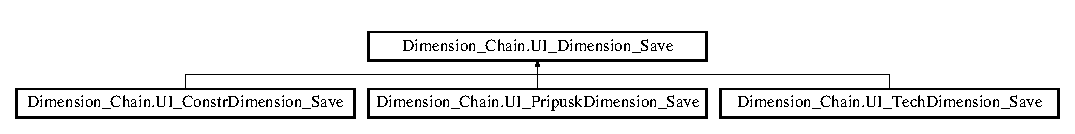
\includegraphics[height=1.352657cm]{class_dimension___chain_1_1_u_i___dimension___save}
\end{center}
\end{figure}
\subsection*{Public Member Functions}
\begin{DoxyCompactItemize}
\item 
\mbox{\hyperlink{class_dimension___chain_1_1_u_i___dimension___save_aae45b10d2ca9f2b9625adf6b1fccb0d4}{U\+I\+\_\+\+Dimension\+\_\+\+Save}} (\mbox{\hyperlink{class_dimension___chain_1_1_u_i___dimension}{U\+I\+\_\+\+Dimension}} dim)
\end{DoxyCompactItemize}
\subsection*{Public Attributes}
\begin{DoxyCompactItemize}
\item 
\mbox{\hyperlink{namespace_dimension___chain_a6ec9051138598c61cc00acf2547dced4}{type}} \mbox{\hyperlink{class_dimension___chain_1_1_u_i___dimension___save_aa786efebf27fc3c4223c35108ffe8876}{typ}}
\item 
double \mbox{\hyperlink{class_dimension___chain_1_1_u_i___dimension___save_ade2ef60cd8d44db6ad2c9be7fa3e40c7}{first\+ElX}}
\item 
double \mbox{\hyperlink{class_dimension___chain_1_1_u_i___dimension___save_a591f5c435d6dd1edc9fe3d91caa888c7}{first\+ElY}}
\item 
double \mbox{\hyperlink{class_dimension___chain_1_1_u_i___dimension___save_a3c51875b880963262a41d8a9e63e1267}{second\+ElX}}
\item 
double \mbox{\hyperlink{class_dimension___chain_1_1_u_i___dimension___save_a28b0b4c78413dd8954d383adc852c034}{second\+ElY}}
\item 
double \mbox{\hyperlink{class_dimension___chain_1_1_u_i___dimension___save_a4d7e3ef8c0639f4c4b10167b94e69d49}{main\+LineY}}
\end{DoxyCompactItemize}


\subsection{Constructor \& Destructor Documentation}
\mbox{\Hypertarget{class_dimension___chain_1_1_u_i___dimension___save_aae45b10d2ca9f2b9625adf6b1fccb0d4}\label{class_dimension___chain_1_1_u_i___dimension___save_aae45b10d2ca9f2b9625adf6b1fccb0d4}} 
\index{Dimension\+\_\+\+Chain\+::\+U\+I\+\_\+\+Dimension\+\_\+\+Save@{Dimension\+\_\+\+Chain\+::\+U\+I\+\_\+\+Dimension\+\_\+\+Save}!U\+I\+\_\+\+Dimension\+\_\+\+Save@{U\+I\+\_\+\+Dimension\+\_\+\+Save}}
\index{U\+I\+\_\+\+Dimension\+\_\+\+Save@{U\+I\+\_\+\+Dimension\+\_\+\+Save}!Dimension\+\_\+\+Chain\+::\+U\+I\+\_\+\+Dimension\+\_\+\+Save@{Dimension\+\_\+\+Chain\+::\+U\+I\+\_\+\+Dimension\+\_\+\+Save}}
\subsubsection{\texorpdfstring{U\+I\+\_\+\+Dimension\+\_\+\+Save()}{UI\_Dimension\_Save()}}
{\footnotesize\ttfamily Dimension\+\_\+\+Chain.\+U\+I\+\_\+\+Dimension\+\_\+\+Save.\+U\+I\+\_\+\+Dimension\+\_\+\+Save (\begin{DoxyParamCaption}\item[{\mbox{\hyperlink{class_dimension___chain_1_1_u_i___dimension}{U\+I\+\_\+\+Dimension}}}]{dim }\end{DoxyParamCaption})}



\subsection{Member Data Documentation}
\mbox{\Hypertarget{class_dimension___chain_1_1_u_i___dimension___save_ade2ef60cd8d44db6ad2c9be7fa3e40c7}\label{class_dimension___chain_1_1_u_i___dimension___save_ade2ef60cd8d44db6ad2c9be7fa3e40c7}} 
\index{Dimension\+\_\+\+Chain\+::\+U\+I\+\_\+\+Dimension\+\_\+\+Save@{Dimension\+\_\+\+Chain\+::\+U\+I\+\_\+\+Dimension\+\_\+\+Save}!first\+ElX@{first\+ElX}}
\index{first\+ElX@{first\+ElX}!Dimension\+\_\+\+Chain\+::\+U\+I\+\_\+\+Dimension\+\_\+\+Save@{Dimension\+\_\+\+Chain\+::\+U\+I\+\_\+\+Dimension\+\_\+\+Save}}
\subsubsection{\texorpdfstring{first\+ElX}{firstElX}}
{\footnotesize\ttfamily double Dimension\+\_\+\+Chain.\+U\+I\+\_\+\+Dimension\+\_\+\+Save.\+first\+ElX}

\mbox{\Hypertarget{class_dimension___chain_1_1_u_i___dimension___save_a591f5c435d6dd1edc9fe3d91caa888c7}\label{class_dimension___chain_1_1_u_i___dimension___save_a591f5c435d6dd1edc9fe3d91caa888c7}} 
\index{Dimension\+\_\+\+Chain\+::\+U\+I\+\_\+\+Dimension\+\_\+\+Save@{Dimension\+\_\+\+Chain\+::\+U\+I\+\_\+\+Dimension\+\_\+\+Save}!first\+ElY@{first\+ElY}}
\index{first\+ElY@{first\+ElY}!Dimension\+\_\+\+Chain\+::\+U\+I\+\_\+\+Dimension\+\_\+\+Save@{Dimension\+\_\+\+Chain\+::\+U\+I\+\_\+\+Dimension\+\_\+\+Save}}
\subsubsection{\texorpdfstring{first\+ElY}{firstElY}}
{\footnotesize\ttfamily double Dimension\+\_\+\+Chain.\+U\+I\+\_\+\+Dimension\+\_\+\+Save.\+first\+ElY}

\mbox{\Hypertarget{class_dimension___chain_1_1_u_i___dimension___save_a4d7e3ef8c0639f4c4b10167b94e69d49}\label{class_dimension___chain_1_1_u_i___dimension___save_a4d7e3ef8c0639f4c4b10167b94e69d49}} 
\index{Dimension\+\_\+\+Chain\+::\+U\+I\+\_\+\+Dimension\+\_\+\+Save@{Dimension\+\_\+\+Chain\+::\+U\+I\+\_\+\+Dimension\+\_\+\+Save}!main\+LineY@{main\+LineY}}
\index{main\+LineY@{main\+LineY}!Dimension\+\_\+\+Chain\+::\+U\+I\+\_\+\+Dimension\+\_\+\+Save@{Dimension\+\_\+\+Chain\+::\+U\+I\+\_\+\+Dimension\+\_\+\+Save}}
\subsubsection{\texorpdfstring{main\+LineY}{mainLineY}}
{\footnotesize\ttfamily double Dimension\+\_\+\+Chain.\+U\+I\+\_\+\+Dimension\+\_\+\+Save.\+main\+LineY}

\mbox{\Hypertarget{class_dimension___chain_1_1_u_i___dimension___save_a3c51875b880963262a41d8a9e63e1267}\label{class_dimension___chain_1_1_u_i___dimension___save_a3c51875b880963262a41d8a9e63e1267}} 
\index{Dimension\+\_\+\+Chain\+::\+U\+I\+\_\+\+Dimension\+\_\+\+Save@{Dimension\+\_\+\+Chain\+::\+U\+I\+\_\+\+Dimension\+\_\+\+Save}!second\+ElX@{second\+ElX}}
\index{second\+ElX@{second\+ElX}!Dimension\+\_\+\+Chain\+::\+U\+I\+\_\+\+Dimension\+\_\+\+Save@{Dimension\+\_\+\+Chain\+::\+U\+I\+\_\+\+Dimension\+\_\+\+Save}}
\subsubsection{\texorpdfstring{second\+ElX}{secondElX}}
{\footnotesize\ttfamily double Dimension\+\_\+\+Chain.\+U\+I\+\_\+\+Dimension\+\_\+\+Save.\+second\+ElX}

\mbox{\Hypertarget{class_dimension___chain_1_1_u_i___dimension___save_a28b0b4c78413dd8954d383adc852c034}\label{class_dimension___chain_1_1_u_i___dimension___save_a28b0b4c78413dd8954d383adc852c034}} 
\index{Dimension\+\_\+\+Chain\+::\+U\+I\+\_\+\+Dimension\+\_\+\+Save@{Dimension\+\_\+\+Chain\+::\+U\+I\+\_\+\+Dimension\+\_\+\+Save}!second\+ElY@{second\+ElY}}
\index{second\+ElY@{second\+ElY}!Dimension\+\_\+\+Chain\+::\+U\+I\+\_\+\+Dimension\+\_\+\+Save@{Dimension\+\_\+\+Chain\+::\+U\+I\+\_\+\+Dimension\+\_\+\+Save}}
\subsubsection{\texorpdfstring{second\+ElY}{secondElY}}
{\footnotesize\ttfamily double Dimension\+\_\+\+Chain.\+U\+I\+\_\+\+Dimension\+\_\+\+Save.\+second\+ElY}

\mbox{\Hypertarget{class_dimension___chain_1_1_u_i___dimension___save_aa786efebf27fc3c4223c35108ffe8876}\label{class_dimension___chain_1_1_u_i___dimension___save_aa786efebf27fc3c4223c35108ffe8876}} 
\index{Dimension\+\_\+\+Chain\+::\+U\+I\+\_\+\+Dimension\+\_\+\+Save@{Dimension\+\_\+\+Chain\+::\+U\+I\+\_\+\+Dimension\+\_\+\+Save}!typ@{typ}}
\index{typ@{typ}!Dimension\+\_\+\+Chain\+::\+U\+I\+\_\+\+Dimension\+\_\+\+Save@{Dimension\+\_\+\+Chain\+::\+U\+I\+\_\+\+Dimension\+\_\+\+Save}}
\subsubsection{\texorpdfstring{typ}{typ}}
{\footnotesize\ttfamily \mbox{\hyperlink{namespace_dimension___chain_a6ec9051138598c61cc00acf2547dced4}{type}} Dimension\+\_\+\+Chain.\+U\+I\+\_\+\+Dimension\+\_\+\+Save.\+typ}



The documentation for this class was generated from the following file\+:\begin{DoxyCompactItemize}
\item 
\mbox{\hyperlink{_save_8cs}{Save.\+cs}}\end{DoxyCompactItemize}

\hypertarget{class_dimension___chain_1_1_u_i___pripusk_dimension}{}\section{Dimension\+\_\+\+Chain.\+U\+I\+\_\+\+Pripusk\+Dimension Class Reference}
\label{class_dimension___chain_1_1_u_i___pripusk_dimension}\index{Dimension\+\_\+\+Chain.\+U\+I\+\_\+\+Pripusk\+Dimension@{Dimension\+\_\+\+Chain.\+U\+I\+\_\+\+Pripusk\+Dimension}}
Inheritance diagram for Dimension\+\_\+\+Chain.\+U\+I\+\_\+\+Pripusk\+Dimension\+:\begin{figure}[H]
\begin{center}
\leavevmode
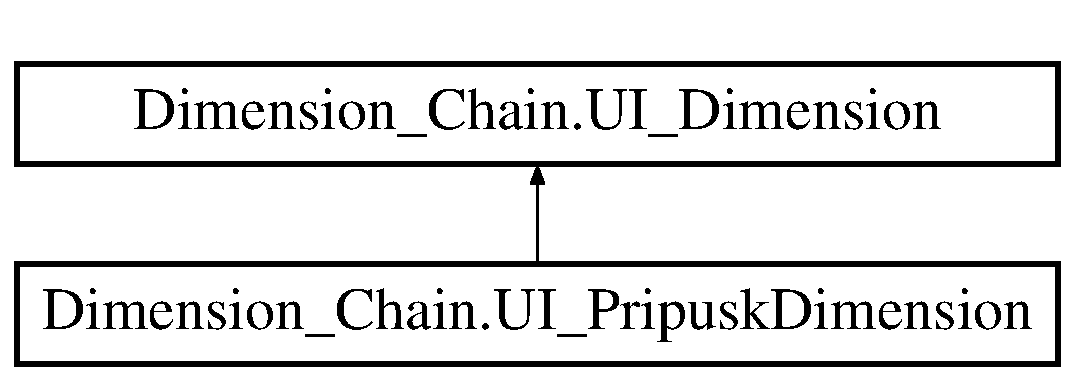
\includegraphics[height=2.000000cm]{class_dimension___chain_1_1_u_i___pripusk_dimension}
\end{center}
\end{figure}
\subsection*{Public Member Functions}
\begin{DoxyCompactItemize}
\item 
\mbox{\hyperlink{class_dimension___chain_1_1_u_i___pripusk_dimension_a1612d83a462124d01e52eb83ca8ca356}{U\+I\+\_\+\+Pripusk\+Dimension}} (\mbox{\hyperlink{class_dimension___chain_1_1_u_i___dimension___save}{U\+I\+\_\+\+Dimension\+\_\+\+Save}} saved)
\item 
delegate void \mbox{\hyperlink{class_dimension___chain_1_1_u_i___pripusk_dimension_a94481db964cf4a247a289d740f916590}{Pripusk\+Apdated\+Event\+Handler}} (\mbox{\hyperlink{class_dimension___chain_1_1_u_i___dimension}{U\+I\+\_\+\+Dimension}} dim)
\item 
\mbox{\hyperlink{class_dimension___chain_1_1_u_i___pripusk_dimension_abf04d49292432d097fb57c417623f27f}{U\+I\+\_\+\+Pripusk\+Dimension}} (\mbox{\hyperlink{class_dimension___chain_1_1_pripusk_user_control}{Pripusk\+User\+Control}} P\+UC)
\item 
override void \mbox{\hyperlink{class_dimension___chain_1_1_u_i___pripusk_dimension_a38ee5caabaa497743eaae261898d12b1}{Set\+Other\+Labels}} ()
\item 
override void \mbox{\hyperlink{class_dimension___chain_1_1_u_i___pripusk_dimension_a463f62358b9a1c671d3cc8c42dc0b6b2}{lbl\+Clicked\+Other\+Podpiska}} ()
\item 
override void \mbox{\hyperlink{class_dimension___chain_1_1_u_i___pripusk_dimension_a68204a8c2d20a3076f2a3bdd3e9bb97a}{Otpiska\+When\+Delate}} ()
\item 
override void \mbox{\hyperlink{class_dimension___chain_1_1_u_i___pripusk_dimension_a38d5be4b36896a5ad78b93c2194a07ac}{Remove\+Other\+Labels}} ()
\item 
override void \mbox{\hyperlink{class_dimension___chain_1_1_u_i___pripusk_dimension_af95139063be522fb5f68e5e0c9945ed2}{Not\+Alarm}} ()
\item 
void \mbox{\hyperlink{class_dimension___chain_1_1_u_i___pripusk_dimension_ab5c8016816db930abd0dc7526e7f2d55}{P\+U\+C\+\_\+\+Apdated}} ()
\end{DoxyCompactItemize}
\subsection*{Public Attributes}
\begin{DoxyCompactItemize}
\item 
double \mbox{\hyperlink{class_dimension___chain_1_1_u_i___pripusk_dimension_ab8f31817ed2cf42d2d645a4d8eb50746}{max}}
\item 
double \mbox{\hyperlink{class_dimension___chain_1_1_u_i___pripusk_dimension_a9f1f95e1d79a7c132271235057375e25}{min}}
\item 
Label \mbox{\hyperlink{class_dimension___chain_1_1_u_i___pripusk_dimension_af2d6a494ea0d7e35b1288a9caaa21ab2}{lbl\+Pripusk}}
\end{DoxyCompactItemize}
\subsection*{Protected Member Functions}
\begin{DoxyCompactItemize}
\item 
void \mbox{\hyperlink{class_dimension___chain_1_1_u_i___pripusk_dimension_a38baa1c8258bfa51eed2800eb90be0c7}{lbl\+Pripusk\+\_\+\+Mouse\+Left\+Button\+Down}} (object sender, Mouse\+Button\+Event\+Args e)
\end{DoxyCompactItemize}
\subsection*{Events}
\begin{DoxyCompactItemize}
\item 
\mbox{\hyperlink{class_dimension___chain_1_1_u_i___pripusk_dimension_a94481db964cf4a247a289d740f916590}{Pripusk\+Apdated\+Event\+Handler}} \mbox{\hyperlink{class_dimension___chain_1_1_u_i___pripusk_dimension_aea5b565f3486e8b370b0deb5ce47fdbc}{Pripusk\+Apdated\+Event}}
\end{DoxyCompactItemize}
\subsection*{Additional Inherited Members}


\subsection{Constructor \& Destructor Documentation}
\mbox{\Hypertarget{class_dimension___chain_1_1_u_i___pripusk_dimension_a1612d83a462124d01e52eb83ca8ca356}\label{class_dimension___chain_1_1_u_i___pripusk_dimension_a1612d83a462124d01e52eb83ca8ca356}} 
\index{Dimension\+\_\+\+Chain\+::\+U\+I\+\_\+\+Pripusk\+Dimension@{Dimension\+\_\+\+Chain\+::\+U\+I\+\_\+\+Pripusk\+Dimension}!U\+I\+\_\+\+Pripusk\+Dimension@{U\+I\+\_\+\+Pripusk\+Dimension}}
\index{U\+I\+\_\+\+Pripusk\+Dimension@{U\+I\+\_\+\+Pripusk\+Dimension}!Dimension\+\_\+\+Chain\+::\+U\+I\+\_\+\+Pripusk\+Dimension@{Dimension\+\_\+\+Chain\+::\+U\+I\+\_\+\+Pripusk\+Dimension}}
\subsubsection{\texorpdfstring{U\+I\+\_\+\+Pripusk\+Dimension()}{UI\_PripuskDimension()}\hspace{0.1cm}{\footnotesize\ttfamily [1/2]}}
{\footnotesize\ttfamily Dimension\+\_\+\+Chain.\+U\+I\+\_\+\+Pripusk\+Dimension.\+U\+I\+\_\+\+Pripusk\+Dimension (\begin{DoxyParamCaption}\item[{\mbox{\hyperlink{class_dimension___chain_1_1_u_i___dimension___save}{U\+I\+\_\+\+Dimension\+\_\+\+Save}}}]{saved }\end{DoxyParamCaption})}

\mbox{\Hypertarget{class_dimension___chain_1_1_u_i___pripusk_dimension_abf04d49292432d097fb57c417623f27f}\label{class_dimension___chain_1_1_u_i___pripusk_dimension_abf04d49292432d097fb57c417623f27f}} 
\index{Dimension\+\_\+\+Chain\+::\+U\+I\+\_\+\+Pripusk\+Dimension@{Dimension\+\_\+\+Chain\+::\+U\+I\+\_\+\+Pripusk\+Dimension}!U\+I\+\_\+\+Pripusk\+Dimension@{U\+I\+\_\+\+Pripusk\+Dimension}}
\index{U\+I\+\_\+\+Pripusk\+Dimension@{U\+I\+\_\+\+Pripusk\+Dimension}!Dimension\+\_\+\+Chain\+::\+U\+I\+\_\+\+Pripusk\+Dimension@{Dimension\+\_\+\+Chain\+::\+U\+I\+\_\+\+Pripusk\+Dimension}}
\subsubsection{\texorpdfstring{U\+I\+\_\+\+Pripusk\+Dimension()}{UI\_PripuskDimension()}\hspace{0.1cm}{\footnotesize\ttfamily [2/2]}}
{\footnotesize\ttfamily Dimension\+\_\+\+Chain.\+U\+I\+\_\+\+Pripusk\+Dimension.\+U\+I\+\_\+\+Pripusk\+Dimension (\begin{DoxyParamCaption}\item[{\mbox{\hyperlink{class_dimension___chain_1_1_pripusk_user_control}{Pripusk\+User\+Control}}}]{P\+UC }\end{DoxyParamCaption})}



\subsection{Member Function Documentation}
\mbox{\Hypertarget{class_dimension___chain_1_1_u_i___pripusk_dimension_a463f62358b9a1c671d3cc8c42dc0b6b2}\label{class_dimension___chain_1_1_u_i___pripusk_dimension_a463f62358b9a1c671d3cc8c42dc0b6b2}} 
\index{Dimension\+\_\+\+Chain\+::\+U\+I\+\_\+\+Pripusk\+Dimension@{Dimension\+\_\+\+Chain\+::\+U\+I\+\_\+\+Pripusk\+Dimension}!lbl\+Clicked\+Other\+Podpiska@{lbl\+Clicked\+Other\+Podpiska}}
\index{lbl\+Clicked\+Other\+Podpiska@{lbl\+Clicked\+Other\+Podpiska}!Dimension\+\_\+\+Chain\+::\+U\+I\+\_\+\+Pripusk\+Dimension@{Dimension\+\_\+\+Chain\+::\+U\+I\+\_\+\+Pripusk\+Dimension}}
\subsubsection{\texorpdfstring{lbl\+Clicked\+Other\+Podpiska()}{lblClickedOtherPodpiska()}}
{\footnotesize\ttfamily override void Dimension\+\_\+\+Chain.\+U\+I\+\_\+\+Pripusk\+Dimension.\+lbl\+Clicked\+Other\+Podpiska (\begin{DoxyParamCaption}{ }\end{DoxyParamCaption})\hspace{0.3cm}{\ttfamily [virtual]}}



Reimplemented from \mbox{\hyperlink{class_dimension___chain_1_1_u_i___dimension_a13210c593c5bd0f5e7b59b93f6ec5fdc}{Dimension\+\_\+\+Chain.\+U\+I\+\_\+\+Dimension}}.

\mbox{\Hypertarget{class_dimension___chain_1_1_u_i___pripusk_dimension_a38baa1c8258bfa51eed2800eb90be0c7}\label{class_dimension___chain_1_1_u_i___pripusk_dimension_a38baa1c8258bfa51eed2800eb90be0c7}} 
\index{Dimension\+\_\+\+Chain\+::\+U\+I\+\_\+\+Pripusk\+Dimension@{Dimension\+\_\+\+Chain\+::\+U\+I\+\_\+\+Pripusk\+Dimension}!lbl\+Pripusk\+\_\+\+Mouse\+Left\+Button\+Down@{lbl\+Pripusk\+\_\+\+Mouse\+Left\+Button\+Down}}
\index{lbl\+Pripusk\+\_\+\+Mouse\+Left\+Button\+Down@{lbl\+Pripusk\+\_\+\+Mouse\+Left\+Button\+Down}!Dimension\+\_\+\+Chain\+::\+U\+I\+\_\+\+Pripusk\+Dimension@{Dimension\+\_\+\+Chain\+::\+U\+I\+\_\+\+Pripusk\+Dimension}}
\subsubsection{\texorpdfstring{lbl\+Pripusk\+\_\+\+Mouse\+Left\+Button\+Down()}{lblPripusk\_MouseLeftButtonDown()}}
{\footnotesize\ttfamily void Dimension\+\_\+\+Chain.\+U\+I\+\_\+\+Pripusk\+Dimension.\+lbl\+Pripusk\+\_\+\+Mouse\+Left\+Button\+Down (\begin{DoxyParamCaption}\item[{object}]{sender,  }\item[{Mouse\+Button\+Event\+Args}]{e }\end{DoxyParamCaption})\hspace{0.3cm}{\ttfamily [protected]}}

\mbox{\Hypertarget{class_dimension___chain_1_1_u_i___pripusk_dimension_af95139063be522fb5f68e5e0c9945ed2}\label{class_dimension___chain_1_1_u_i___pripusk_dimension_af95139063be522fb5f68e5e0c9945ed2}} 
\index{Dimension\+\_\+\+Chain\+::\+U\+I\+\_\+\+Pripusk\+Dimension@{Dimension\+\_\+\+Chain\+::\+U\+I\+\_\+\+Pripusk\+Dimension}!Not\+Alarm@{Not\+Alarm}}
\index{Not\+Alarm@{Not\+Alarm}!Dimension\+\_\+\+Chain\+::\+U\+I\+\_\+\+Pripusk\+Dimension@{Dimension\+\_\+\+Chain\+::\+U\+I\+\_\+\+Pripusk\+Dimension}}
\subsubsection{\texorpdfstring{Not\+Alarm()}{NotAlarm()}}
{\footnotesize\ttfamily override void Dimension\+\_\+\+Chain.\+U\+I\+\_\+\+Pripusk\+Dimension.\+Not\+Alarm (\begin{DoxyParamCaption}{ }\end{DoxyParamCaption})\hspace{0.3cm}{\ttfamily [virtual]}}



Reimplemented from \mbox{\hyperlink{class_dimension___chain_1_1_u_i___dimension_a4ab4c36c068571222229db5f0a194dd2}{Dimension\+\_\+\+Chain.\+U\+I\+\_\+\+Dimension}}.

\mbox{\Hypertarget{class_dimension___chain_1_1_u_i___pripusk_dimension_a68204a8c2d20a3076f2a3bdd3e9bb97a}\label{class_dimension___chain_1_1_u_i___pripusk_dimension_a68204a8c2d20a3076f2a3bdd3e9bb97a}} 
\index{Dimension\+\_\+\+Chain\+::\+U\+I\+\_\+\+Pripusk\+Dimension@{Dimension\+\_\+\+Chain\+::\+U\+I\+\_\+\+Pripusk\+Dimension}!Otpiska\+When\+Delate@{Otpiska\+When\+Delate}}
\index{Otpiska\+When\+Delate@{Otpiska\+When\+Delate}!Dimension\+\_\+\+Chain\+::\+U\+I\+\_\+\+Pripusk\+Dimension@{Dimension\+\_\+\+Chain\+::\+U\+I\+\_\+\+Pripusk\+Dimension}}
\subsubsection{\texorpdfstring{Otpiska\+When\+Delate()}{OtpiskaWhenDelate()}}
{\footnotesize\ttfamily override void Dimension\+\_\+\+Chain.\+U\+I\+\_\+\+Pripusk\+Dimension.\+Otpiska\+When\+Delate (\begin{DoxyParamCaption}{ }\end{DoxyParamCaption})\hspace{0.3cm}{\ttfamily [virtual]}}



Reimplemented from \mbox{\hyperlink{class_dimension___chain_1_1_u_i___dimension_aad38da2794443edfca137c15e417bfd3}{Dimension\+\_\+\+Chain.\+U\+I\+\_\+\+Dimension}}.

\mbox{\Hypertarget{class_dimension___chain_1_1_u_i___pripusk_dimension_a94481db964cf4a247a289d740f916590}\label{class_dimension___chain_1_1_u_i___pripusk_dimension_a94481db964cf4a247a289d740f916590}} 
\index{Dimension\+\_\+\+Chain\+::\+U\+I\+\_\+\+Pripusk\+Dimension@{Dimension\+\_\+\+Chain\+::\+U\+I\+\_\+\+Pripusk\+Dimension}!Pripusk\+Apdated\+Event\+Handler@{Pripusk\+Apdated\+Event\+Handler}}
\index{Pripusk\+Apdated\+Event\+Handler@{Pripusk\+Apdated\+Event\+Handler}!Dimension\+\_\+\+Chain\+::\+U\+I\+\_\+\+Pripusk\+Dimension@{Dimension\+\_\+\+Chain\+::\+U\+I\+\_\+\+Pripusk\+Dimension}}
\subsubsection{\texorpdfstring{Pripusk\+Apdated\+Event\+Handler()}{PripuskApdatedEventHandler()}}
{\footnotesize\ttfamily delegate void Dimension\+\_\+\+Chain.\+U\+I\+\_\+\+Pripusk\+Dimension.\+Pripusk\+Apdated\+Event\+Handler (\begin{DoxyParamCaption}\item[{\mbox{\hyperlink{class_dimension___chain_1_1_u_i___dimension}{U\+I\+\_\+\+Dimension}}}]{dim }\end{DoxyParamCaption})}

\mbox{\Hypertarget{class_dimension___chain_1_1_u_i___pripusk_dimension_ab5c8016816db930abd0dc7526e7f2d55}\label{class_dimension___chain_1_1_u_i___pripusk_dimension_ab5c8016816db930abd0dc7526e7f2d55}} 
\index{Dimension\+\_\+\+Chain\+::\+U\+I\+\_\+\+Pripusk\+Dimension@{Dimension\+\_\+\+Chain\+::\+U\+I\+\_\+\+Pripusk\+Dimension}!P\+U\+C\+\_\+\+Apdated@{P\+U\+C\+\_\+\+Apdated}}
\index{P\+U\+C\+\_\+\+Apdated@{P\+U\+C\+\_\+\+Apdated}!Dimension\+\_\+\+Chain\+::\+U\+I\+\_\+\+Pripusk\+Dimension@{Dimension\+\_\+\+Chain\+::\+U\+I\+\_\+\+Pripusk\+Dimension}}
\subsubsection{\texorpdfstring{P\+U\+C\+\_\+\+Apdated()}{PUC\_Apdated()}}
{\footnotesize\ttfamily void Dimension\+\_\+\+Chain.\+U\+I\+\_\+\+Pripusk\+Dimension.\+P\+U\+C\+\_\+\+Apdated (\begin{DoxyParamCaption}{ }\end{DoxyParamCaption})}

\mbox{\Hypertarget{class_dimension___chain_1_1_u_i___pripusk_dimension_a38d5be4b36896a5ad78b93c2194a07ac}\label{class_dimension___chain_1_1_u_i___pripusk_dimension_a38d5be4b36896a5ad78b93c2194a07ac}} 
\index{Dimension\+\_\+\+Chain\+::\+U\+I\+\_\+\+Pripusk\+Dimension@{Dimension\+\_\+\+Chain\+::\+U\+I\+\_\+\+Pripusk\+Dimension}!Remove\+Other\+Labels@{Remove\+Other\+Labels}}
\index{Remove\+Other\+Labels@{Remove\+Other\+Labels}!Dimension\+\_\+\+Chain\+::\+U\+I\+\_\+\+Pripusk\+Dimension@{Dimension\+\_\+\+Chain\+::\+U\+I\+\_\+\+Pripusk\+Dimension}}
\subsubsection{\texorpdfstring{Remove\+Other\+Labels()}{RemoveOtherLabels()}}
{\footnotesize\ttfamily override void Dimension\+\_\+\+Chain.\+U\+I\+\_\+\+Pripusk\+Dimension.\+Remove\+Other\+Labels (\begin{DoxyParamCaption}{ }\end{DoxyParamCaption})\hspace{0.3cm}{\ttfamily [virtual]}}



Reimplemented from \mbox{\hyperlink{class_dimension___chain_1_1_u_i___dimension_a17854a85eba47798b7459b633f1db4bb}{Dimension\+\_\+\+Chain.\+U\+I\+\_\+\+Dimension}}.

\mbox{\Hypertarget{class_dimension___chain_1_1_u_i___pripusk_dimension_a38ee5caabaa497743eaae261898d12b1}\label{class_dimension___chain_1_1_u_i___pripusk_dimension_a38ee5caabaa497743eaae261898d12b1}} 
\index{Dimension\+\_\+\+Chain\+::\+U\+I\+\_\+\+Pripusk\+Dimension@{Dimension\+\_\+\+Chain\+::\+U\+I\+\_\+\+Pripusk\+Dimension}!Set\+Other\+Labels@{Set\+Other\+Labels}}
\index{Set\+Other\+Labels@{Set\+Other\+Labels}!Dimension\+\_\+\+Chain\+::\+U\+I\+\_\+\+Pripusk\+Dimension@{Dimension\+\_\+\+Chain\+::\+U\+I\+\_\+\+Pripusk\+Dimension}}
\subsubsection{\texorpdfstring{Set\+Other\+Labels()}{SetOtherLabels()}}
{\footnotesize\ttfamily override void Dimension\+\_\+\+Chain.\+U\+I\+\_\+\+Pripusk\+Dimension.\+Set\+Other\+Labels (\begin{DoxyParamCaption}{ }\end{DoxyParamCaption})\hspace{0.3cm}{\ttfamily [virtual]}}



Reimplemented from \mbox{\hyperlink{class_dimension___chain_1_1_u_i___dimension_a78774f971a6494a57310623f4bf0aa4f}{Dimension\+\_\+\+Chain.\+U\+I\+\_\+\+Dimension}}.



\subsection{Member Data Documentation}
\mbox{\Hypertarget{class_dimension___chain_1_1_u_i___pripusk_dimension_af2d6a494ea0d7e35b1288a9caaa21ab2}\label{class_dimension___chain_1_1_u_i___pripusk_dimension_af2d6a494ea0d7e35b1288a9caaa21ab2}} 
\index{Dimension\+\_\+\+Chain\+::\+U\+I\+\_\+\+Pripusk\+Dimension@{Dimension\+\_\+\+Chain\+::\+U\+I\+\_\+\+Pripusk\+Dimension}!lbl\+Pripusk@{lbl\+Pripusk}}
\index{lbl\+Pripusk@{lbl\+Pripusk}!Dimension\+\_\+\+Chain\+::\+U\+I\+\_\+\+Pripusk\+Dimension@{Dimension\+\_\+\+Chain\+::\+U\+I\+\_\+\+Pripusk\+Dimension}}
\subsubsection{\texorpdfstring{lbl\+Pripusk}{lblPripusk}}
{\footnotesize\ttfamily Label Dimension\+\_\+\+Chain.\+U\+I\+\_\+\+Pripusk\+Dimension.\+lbl\+Pripusk}

\mbox{\Hypertarget{class_dimension___chain_1_1_u_i___pripusk_dimension_ab8f31817ed2cf42d2d645a4d8eb50746}\label{class_dimension___chain_1_1_u_i___pripusk_dimension_ab8f31817ed2cf42d2d645a4d8eb50746}} 
\index{Dimension\+\_\+\+Chain\+::\+U\+I\+\_\+\+Pripusk\+Dimension@{Dimension\+\_\+\+Chain\+::\+U\+I\+\_\+\+Pripusk\+Dimension}!max@{max}}
\index{max@{max}!Dimension\+\_\+\+Chain\+::\+U\+I\+\_\+\+Pripusk\+Dimension@{Dimension\+\_\+\+Chain\+::\+U\+I\+\_\+\+Pripusk\+Dimension}}
\subsubsection{\texorpdfstring{max}{max}}
{\footnotesize\ttfamily double Dimension\+\_\+\+Chain.\+U\+I\+\_\+\+Pripusk\+Dimension.\+max}

\mbox{\Hypertarget{class_dimension___chain_1_1_u_i___pripusk_dimension_a9f1f95e1d79a7c132271235057375e25}\label{class_dimension___chain_1_1_u_i___pripusk_dimension_a9f1f95e1d79a7c132271235057375e25}} 
\index{Dimension\+\_\+\+Chain\+::\+U\+I\+\_\+\+Pripusk\+Dimension@{Dimension\+\_\+\+Chain\+::\+U\+I\+\_\+\+Pripusk\+Dimension}!min@{min}}
\index{min@{min}!Dimension\+\_\+\+Chain\+::\+U\+I\+\_\+\+Pripusk\+Dimension@{Dimension\+\_\+\+Chain\+::\+U\+I\+\_\+\+Pripusk\+Dimension}}
\subsubsection{\texorpdfstring{min}{min}}
{\footnotesize\ttfamily double Dimension\+\_\+\+Chain.\+U\+I\+\_\+\+Pripusk\+Dimension.\+min}



\subsection{Event Documentation}
\mbox{\Hypertarget{class_dimension___chain_1_1_u_i___pripusk_dimension_aea5b565f3486e8b370b0deb5ce47fdbc}\label{class_dimension___chain_1_1_u_i___pripusk_dimension_aea5b565f3486e8b370b0deb5ce47fdbc}} 
\index{Dimension\+\_\+\+Chain\+::\+U\+I\+\_\+\+Pripusk\+Dimension@{Dimension\+\_\+\+Chain\+::\+U\+I\+\_\+\+Pripusk\+Dimension}!Pripusk\+Apdated\+Event@{Pripusk\+Apdated\+Event}}
\index{Pripusk\+Apdated\+Event@{Pripusk\+Apdated\+Event}!Dimension\+\_\+\+Chain\+::\+U\+I\+\_\+\+Pripusk\+Dimension@{Dimension\+\_\+\+Chain\+::\+U\+I\+\_\+\+Pripusk\+Dimension}}
\subsubsection{\texorpdfstring{Pripusk\+Apdated\+Event}{PripuskApdatedEvent}}
{\footnotesize\ttfamily \mbox{\hyperlink{class_dimension___chain_1_1_u_i___pripusk_dimension_a94481db964cf4a247a289d740f916590}{Pripusk\+Apdated\+Event\+Handler}} Dimension\+\_\+\+Chain.\+U\+I\+\_\+\+Pripusk\+Dimension.\+Pripusk\+Apdated\+Event}



The documentation for this class was generated from the following files\+:\begin{DoxyCompactItemize}
\item 
\mbox{\hyperlink{_u_i___dimension_partial_8cs}{U\+I\+\_\+\+Dimension\+Partial.\+cs}}\item 
\mbox{\hyperlink{_u_i___pripusk_dimension_8cs}{U\+I\+\_\+\+Pripusk\+Dimension.\+cs}}\end{DoxyCompactItemize}

\hypertarget{class_dimension___chain_1_1_u_i___pripusk_dimension___save}{}\section{Dimension\+\_\+\+Chain.\+U\+I\+\_\+\+Pripusk\+Dimension\+\_\+\+Save Class Reference}
\label{class_dimension___chain_1_1_u_i___pripusk_dimension___save}\index{Dimension\+\_\+\+Chain.\+U\+I\+\_\+\+Pripusk\+Dimension\+\_\+\+Save@{Dimension\+\_\+\+Chain.\+U\+I\+\_\+\+Pripusk\+Dimension\+\_\+\+Save}}
Inheritance diagram for Dimension\+\_\+\+Chain.\+U\+I\+\_\+\+Pripusk\+Dimension\+\_\+\+Save\+:\begin{figure}[H]
\begin{center}
\leavevmode
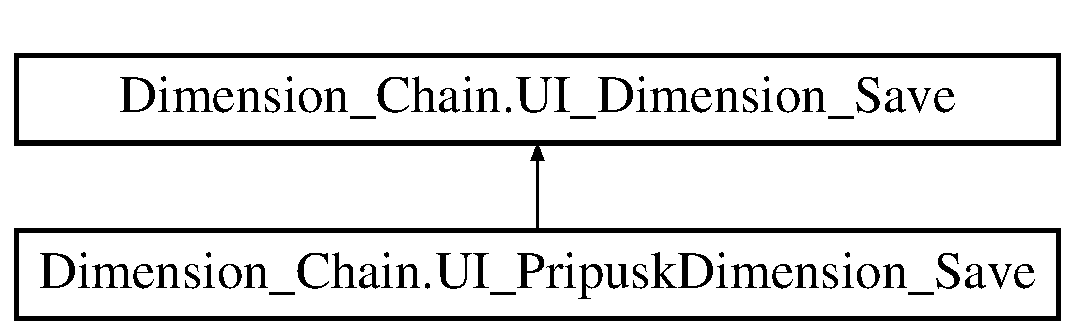
\includegraphics[height=2.000000cm]{class_dimension___chain_1_1_u_i___pripusk_dimension___save}
\end{center}
\end{figure}
\subsection*{Public Member Functions}
\begin{DoxyCompactItemize}
\item 
\mbox{\hyperlink{class_dimension___chain_1_1_u_i___pripusk_dimension___save_a5eaa1096da02b3f5dff6c6a2a8f0237d}{U\+I\+\_\+\+Pripusk\+Dimension\+\_\+\+Save}} (\mbox{\hyperlink{class_dimension___chain_1_1_u_i___pripusk_dimension}{U\+I\+\_\+\+Pripusk\+Dimension}} dim)
\end{DoxyCompactItemize}
\subsection*{Public Attributes}
\begin{DoxyCompactItemize}
\item 
double \mbox{\hyperlink{class_dimension___chain_1_1_u_i___pripusk_dimension___save_aaa4e1820ebace0d4cf7952bae2b8d012}{max}}
\item 
double \mbox{\hyperlink{class_dimension___chain_1_1_u_i___pripusk_dimension___save_a80d76285a268b8b24dba1c8d5160133a}{min}}
\end{DoxyCompactItemize}


\subsection{Constructor \& Destructor Documentation}
\mbox{\Hypertarget{class_dimension___chain_1_1_u_i___pripusk_dimension___save_a5eaa1096da02b3f5dff6c6a2a8f0237d}\label{class_dimension___chain_1_1_u_i___pripusk_dimension___save_a5eaa1096da02b3f5dff6c6a2a8f0237d}} 
\index{Dimension\+\_\+\+Chain\+::\+U\+I\+\_\+\+Pripusk\+Dimension\+\_\+\+Save@{Dimension\+\_\+\+Chain\+::\+U\+I\+\_\+\+Pripusk\+Dimension\+\_\+\+Save}!U\+I\+\_\+\+Pripusk\+Dimension\+\_\+\+Save@{U\+I\+\_\+\+Pripusk\+Dimension\+\_\+\+Save}}
\index{U\+I\+\_\+\+Pripusk\+Dimension\+\_\+\+Save@{U\+I\+\_\+\+Pripusk\+Dimension\+\_\+\+Save}!Dimension\+\_\+\+Chain\+::\+U\+I\+\_\+\+Pripusk\+Dimension\+\_\+\+Save@{Dimension\+\_\+\+Chain\+::\+U\+I\+\_\+\+Pripusk\+Dimension\+\_\+\+Save}}
\subsubsection{\texorpdfstring{U\+I\+\_\+\+Pripusk\+Dimension\+\_\+\+Save()}{UI\_PripuskDimension\_Save()}}
{\footnotesize\ttfamily Dimension\+\_\+\+Chain.\+U\+I\+\_\+\+Pripusk\+Dimension\+\_\+\+Save.\+U\+I\+\_\+\+Pripusk\+Dimension\+\_\+\+Save (\begin{DoxyParamCaption}\item[{\mbox{\hyperlink{class_dimension___chain_1_1_u_i___pripusk_dimension}{U\+I\+\_\+\+Pripusk\+Dimension}}}]{dim }\end{DoxyParamCaption})}



\subsection{Member Data Documentation}
\mbox{\Hypertarget{class_dimension___chain_1_1_u_i___pripusk_dimension___save_aaa4e1820ebace0d4cf7952bae2b8d012}\label{class_dimension___chain_1_1_u_i___pripusk_dimension___save_aaa4e1820ebace0d4cf7952bae2b8d012}} 
\index{Dimension\+\_\+\+Chain\+::\+U\+I\+\_\+\+Pripusk\+Dimension\+\_\+\+Save@{Dimension\+\_\+\+Chain\+::\+U\+I\+\_\+\+Pripusk\+Dimension\+\_\+\+Save}!max@{max}}
\index{max@{max}!Dimension\+\_\+\+Chain\+::\+U\+I\+\_\+\+Pripusk\+Dimension\+\_\+\+Save@{Dimension\+\_\+\+Chain\+::\+U\+I\+\_\+\+Pripusk\+Dimension\+\_\+\+Save}}
\subsubsection{\texorpdfstring{max}{max}}
{\footnotesize\ttfamily double Dimension\+\_\+\+Chain.\+U\+I\+\_\+\+Pripusk\+Dimension\+\_\+\+Save.\+max}

\mbox{\Hypertarget{class_dimension___chain_1_1_u_i___pripusk_dimension___save_a80d76285a268b8b24dba1c8d5160133a}\label{class_dimension___chain_1_1_u_i___pripusk_dimension___save_a80d76285a268b8b24dba1c8d5160133a}} 
\index{Dimension\+\_\+\+Chain\+::\+U\+I\+\_\+\+Pripusk\+Dimension\+\_\+\+Save@{Dimension\+\_\+\+Chain\+::\+U\+I\+\_\+\+Pripusk\+Dimension\+\_\+\+Save}!min@{min}}
\index{min@{min}!Dimension\+\_\+\+Chain\+::\+U\+I\+\_\+\+Pripusk\+Dimension\+\_\+\+Save@{Dimension\+\_\+\+Chain\+::\+U\+I\+\_\+\+Pripusk\+Dimension\+\_\+\+Save}}
\subsubsection{\texorpdfstring{min}{min}}
{\footnotesize\ttfamily double Dimension\+\_\+\+Chain.\+U\+I\+\_\+\+Pripusk\+Dimension\+\_\+\+Save.\+min}



The documentation for this class was generated from the following file\+:\begin{DoxyCompactItemize}
\item 
\mbox{\hyperlink{_save_8cs}{Save.\+cs}}\end{DoxyCompactItemize}

\hypertarget{class_dimension___chain_1_1_u_i___tech_dimension}{}\section{Dimension\+\_\+\+Chain.\+U\+I\+\_\+\+Tech\+Dimension Class Reference}
\label{class_dimension___chain_1_1_u_i___tech_dimension}\index{Dimension\+\_\+\+Chain.\+U\+I\+\_\+\+Tech\+Dimension@{Dimension\+\_\+\+Chain.\+U\+I\+\_\+\+Tech\+Dimension}}
Inheritance diagram for Dimension\+\_\+\+Chain.\+U\+I\+\_\+\+Tech\+Dimension\+:\begin{figure}[H]
\begin{center}
\leavevmode
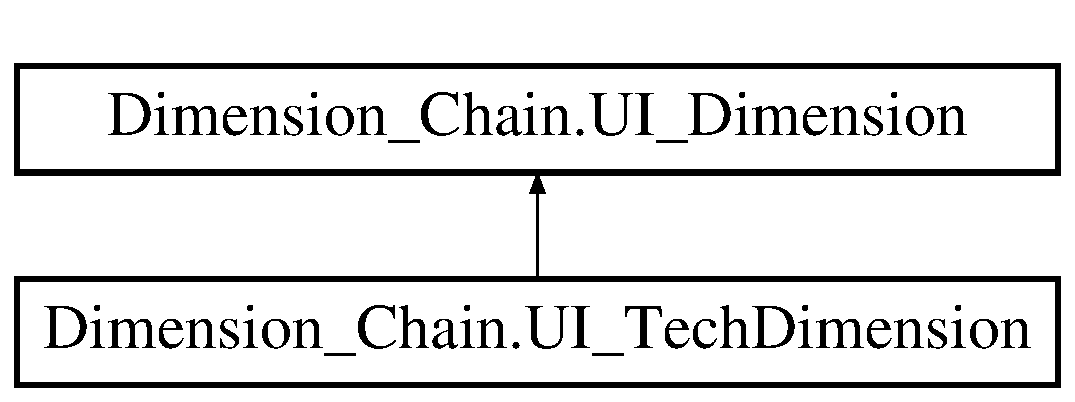
\includegraphics[height=2.000000cm]{class_dimension___chain_1_1_u_i___tech_dimension}
\end{center}
\end{figure}
\subsection*{Public Member Functions}
\begin{DoxyCompactItemize}
\item 
\mbox{\hyperlink{class_dimension___chain_1_1_u_i___tech_dimension_a8075dce6b26f265a61725c27a636aa38}{U\+I\+\_\+\+Tech\+Dimension}} (\mbox{\hyperlink{class_dimension___chain_1_1_u_i___dimension___save}{U\+I\+\_\+\+Dimension\+\_\+\+Save}} saved)
\item 
delegate void \mbox{\hyperlink{class_dimension___chain_1_1_u_i___tech_dimension_a55a3d4e5dad3a8b18f8bffb9adf5cb6f}{Tech\+Dimension\+Apdated\+Event\+Handler}} (\mbox{\hyperlink{class_dimension___chain_1_1_u_i___tech_dimension}{U\+I\+\_\+\+Tech\+Dimension}} dim)
\item 
\mbox{\hyperlink{class_dimension___chain_1_1_u_i___tech_dimension_a08e8bf66ff37909eb567ef9fddb0fb03}{U\+I\+\_\+\+Tech\+Dimension}} (\mbox{\hyperlink{class_dimension___chain_1_1_tech_user_control}{Tech\+User\+Control}} T\+UC)
\item 
void \mbox{\hyperlink{class_dimension___chain_1_1_u_i___tech_dimension_ade84015225ae3cd225d1db4e2c78b42c}{T\+U\+C\+\_\+\+Apdated}} ()
\item 
override void \mbox{\hyperlink{class_dimension___chain_1_1_u_i___tech_dimension_a4c37ac44bbc3b0fdf564e42961353a5f}{Otpiska\+When\+Delate}} ()
\item 
override void \mbox{\hyperlink{class_dimension___chain_1_1_u_i___tech_dimension_a7b8198570ba66a56ef0c78a8550916d2}{Remove\+Other\+Labels}} ()
\item 
override void \mbox{\hyperlink{class_dimension___chain_1_1_u_i___tech_dimension_a36fd2ba82028e120d68819acc5c50daf}{Unchoose}} ()
\end{DoxyCompactItemize}
\subsection*{Events}
\begin{DoxyCompactItemize}
\item 
\mbox{\hyperlink{class_dimension___chain_1_1_u_i___tech_dimension_a55a3d4e5dad3a8b18f8bffb9adf5cb6f}{Tech\+Dimension\+Apdated\+Event\+Handler}} \mbox{\hyperlink{class_dimension___chain_1_1_u_i___tech_dimension_a8bb9c9ee3e838f322941a839e37b9799}{Tech\+Dimension\+Apdated\+Event}}
\end{DoxyCompactItemize}
\subsection*{Additional Inherited Members}


\subsection{Constructor \& Destructor Documentation}
\mbox{\Hypertarget{class_dimension___chain_1_1_u_i___tech_dimension_a8075dce6b26f265a61725c27a636aa38}\label{class_dimension___chain_1_1_u_i___tech_dimension_a8075dce6b26f265a61725c27a636aa38}} 
\index{Dimension\+\_\+\+Chain\+::\+U\+I\+\_\+\+Tech\+Dimension@{Dimension\+\_\+\+Chain\+::\+U\+I\+\_\+\+Tech\+Dimension}!U\+I\+\_\+\+Tech\+Dimension@{U\+I\+\_\+\+Tech\+Dimension}}
\index{U\+I\+\_\+\+Tech\+Dimension@{U\+I\+\_\+\+Tech\+Dimension}!Dimension\+\_\+\+Chain\+::\+U\+I\+\_\+\+Tech\+Dimension@{Dimension\+\_\+\+Chain\+::\+U\+I\+\_\+\+Tech\+Dimension}}
\subsubsection{\texorpdfstring{U\+I\+\_\+\+Tech\+Dimension()}{UI\_TechDimension()}\hspace{0.1cm}{\footnotesize\ttfamily [1/2]}}
{\footnotesize\ttfamily Dimension\+\_\+\+Chain.\+U\+I\+\_\+\+Tech\+Dimension.\+U\+I\+\_\+\+Tech\+Dimension (\begin{DoxyParamCaption}\item[{\mbox{\hyperlink{class_dimension___chain_1_1_u_i___dimension___save}{U\+I\+\_\+\+Dimension\+\_\+\+Save}}}]{saved }\end{DoxyParamCaption})}

\mbox{\Hypertarget{class_dimension___chain_1_1_u_i___tech_dimension_a08e8bf66ff37909eb567ef9fddb0fb03}\label{class_dimension___chain_1_1_u_i___tech_dimension_a08e8bf66ff37909eb567ef9fddb0fb03}} 
\index{Dimension\+\_\+\+Chain\+::\+U\+I\+\_\+\+Tech\+Dimension@{Dimension\+\_\+\+Chain\+::\+U\+I\+\_\+\+Tech\+Dimension}!U\+I\+\_\+\+Tech\+Dimension@{U\+I\+\_\+\+Tech\+Dimension}}
\index{U\+I\+\_\+\+Tech\+Dimension@{U\+I\+\_\+\+Tech\+Dimension}!Dimension\+\_\+\+Chain\+::\+U\+I\+\_\+\+Tech\+Dimension@{Dimension\+\_\+\+Chain\+::\+U\+I\+\_\+\+Tech\+Dimension}}
\subsubsection{\texorpdfstring{U\+I\+\_\+\+Tech\+Dimension()}{UI\_TechDimension()}\hspace{0.1cm}{\footnotesize\ttfamily [2/2]}}
{\footnotesize\ttfamily Dimension\+\_\+\+Chain.\+U\+I\+\_\+\+Tech\+Dimension.\+U\+I\+\_\+\+Tech\+Dimension (\begin{DoxyParamCaption}\item[{\mbox{\hyperlink{class_dimension___chain_1_1_tech_user_control}{Tech\+User\+Control}}}]{T\+UC }\end{DoxyParamCaption})}



\subsection{Member Function Documentation}
\mbox{\Hypertarget{class_dimension___chain_1_1_u_i___tech_dimension_a4c37ac44bbc3b0fdf564e42961353a5f}\label{class_dimension___chain_1_1_u_i___tech_dimension_a4c37ac44bbc3b0fdf564e42961353a5f}} 
\index{Dimension\+\_\+\+Chain\+::\+U\+I\+\_\+\+Tech\+Dimension@{Dimension\+\_\+\+Chain\+::\+U\+I\+\_\+\+Tech\+Dimension}!Otpiska\+When\+Delate@{Otpiska\+When\+Delate}}
\index{Otpiska\+When\+Delate@{Otpiska\+When\+Delate}!Dimension\+\_\+\+Chain\+::\+U\+I\+\_\+\+Tech\+Dimension@{Dimension\+\_\+\+Chain\+::\+U\+I\+\_\+\+Tech\+Dimension}}
\subsubsection{\texorpdfstring{Otpiska\+When\+Delate()}{OtpiskaWhenDelate()}}
{\footnotesize\ttfamily override void Dimension\+\_\+\+Chain.\+U\+I\+\_\+\+Tech\+Dimension.\+Otpiska\+When\+Delate (\begin{DoxyParamCaption}{ }\end{DoxyParamCaption})\hspace{0.3cm}{\ttfamily [virtual]}}



Reimplemented from \mbox{\hyperlink{class_dimension___chain_1_1_u_i___dimension_aad38da2794443edfca137c15e417bfd3}{Dimension\+\_\+\+Chain.\+U\+I\+\_\+\+Dimension}}.

\mbox{\Hypertarget{class_dimension___chain_1_1_u_i___tech_dimension_a7b8198570ba66a56ef0c78a8550916d2}\label{class_dimension___chain_1_1_u_i___tech_dimension_a7b8198570ba66a56ef0c78a8550916d2}} 
\index{Dimension\+\_\+\+Chain\+::\+U\+I\+\_\+\+Tech\+Dimension@{Dimension\+\_\+\+Chain\+::\+U\+I\+\_\+\+Tech\+Dimension}!Remove\+Other\+Labels@{Remove\+Other\+Labels}}
\index{Remove\+Other\+Labels@{Remove\+Other\+Labels}!Dimension\+\_\+\+Chain\+::\+U\+I\+\_\+\+Tech\+Dimension@{Dimension\+\_\+\+Chain\+::\+U\+I\+\_\+\+Tech\+Dimension}}
\subsubsection{\texorpdfstring{Remove\+Other\+Labels()}{RemoveOtherLabels()}}
{\footnotesize\ttfamily override void Dimension\+\_\+\+Chain.\+U\+I\+\_\+\+Tech\+Dimension.\+Remove\+Other\+Labels (\begin{DoxyParamCaption}{ }\end{DoxyParamCaption})\hspace{0.3cm}{\ttfamily [virtual]}}



Reimplemented from \mbox{\hyperlink{class_dimension___chain_1_1_u_i___dimension_a17854a85eba47798b7459b633f1db4bb}{Dimension\+\_\+\+Chain.\+U\+I\+\_\+\+Dimension}}.

\mbox{\Hypertarget{class_dimension___chain_1_1_u_i___tech_dimension_a55a3d4e5dad3a8b18f8bffb9adf5cb6f}\label{class_dimension___chain_1_1_u_i___tech_dimension_a55a3d4e5dad3a8b18f8bffb9adf5cb6f}} 
\index{Dimension\+\_\+\+Chain\+::\+U\+I\+\_\+\+Tech\+Dimension@{Dimension\+\_\+\+Chain\+::\+U\+I\+\_\+\+Tech\+Dimension}!Tech\+Dimension\+Apdated\+Event\+Handler@{Tech\+Dimension\+Apdated\+Event\+Handler}}
\index{Tech\+Dimension\+Apdated\+Event\+Handler@{Tech\+Dimension\+Apdated\+Event\+Handler}!Dimension\+\_\+\+Chain\+::\+U\+I\+\_\+\+Tech\+Dimension@{Dimension\+\_\+\+Chain\+::\+U\+I\+\_\+\+Tech\+Dimension}}
\subsubsection{\texorpdfstring{Tech\+Dimension\+Apdated\+Event\+Handler()}{TechDimensionApdatedEventHandler()}}
{\footnotesize\ttfamily delegate void Dimension\+\_\+\+Chain.\+U\+I\+\_\+\+Tech\+Dimension.\+Tech\+Dimension\+Apdated\+Event\+Handler (\begin{DoxyParamCaption}\item[{\mbox{\hyperlink{class_dimension___chain_1_1_u_i___tech_dimension}{U\+I\+\_\+\+Tech\+Dimension}}}]{dim }\end{DoxyParamCaption})}

\mbox{\Hypertarget{class_dimension___chain_1_1_u_i___tech_dimension_ade84015225ae3cd225d1db4e2c78b42c}\label{class_dimension___chain_1_1_u_i___tech_dimension_ade84015225ae3cd225d1db4e2c78b42c}} 
\index{Dimension\+\_\+\+Chain\+::\+U\+I\+\_\+\+Tech\+Dimension@{Dimension\+\_\+\+Chain\+::\+U\+I\+\_\+\+Tech\+Dimension}!T\+U\+C\+\_\+\+Apdated@{T\+U\+C\+\_\+\+Apdated}}
\index{T\+U\+C\+\_\+\+Apdated@{T\+U\+C\+\_\+\+Apdated}!Dimension\+\_\+\+Chain\+::\+U\+I\+\_\+\+Tech\+Dimension@{Dimension\+\_\+\+Chain\+::\+U\+I\+\_\+\+Tech\+Dimension}}
\subsubsection{\texorpdfstring{T\+U\+C\+\_\+\+Apdated()}{TUC\_Apdated()}}
{\footnotesize\ttfamily void Dimension\+\_\+\+Chain.\+U\+I\+\_\+\+Tech\+Dimension.\+T\+U\+C\+\_\+\+Apdated (\begin{DoxyParamCaption}{ }\end{DoxyParamCaption})}

\mbox{\Hypertarget{class_dimension___chain_1_1_u_i___tech_dimension_a36fd2ba82028e120d68819acc5c50daf}\label{class_dimension___chain_1_1_u_i___tech_dimension_a36fd2ba82028e120d68819acc5c50daf}} 
\index{Dimension\+\_\+\+Chain\+::\+U\+I\+\_\+\+Tech\+Dimension@{Dimension\+\_\+\+Chain\+::\+U\+I\+\_\+\+Tech\+Dimension}!Unchoose@{Unchoose}}
\index{Unchoose@{Unchoose}!Dimension\+\_\+\+Chain\+::\+U\+I\+\_\+\+Tech\+Dimension@{Dimension\+\_\+\+Chain\+::\+U\+I\+\_\+\+Tech\+Dimension}}
\subsubsection{\texorpdfstring{Unchoose()}{Unchoose()}}
{\footnotesize\ttfamily override void Dimension\+\_\+\+Chain.\+U\+I\+\_\+\+Tech\+Dimension.\+Unchoose (\begin{DoxyParamCaption}{ }\end{DoxyParamCaption})\hspace{0.3cm}{\ttfamily [virtual]}}



Reimplemented from \mbox{\hyperlink{class_dimension___chain_1_1_u_i___dimension_a93110c560bdd2e03e4a943be85a0f913}{Dimension\+\_\+\+Chain.\+U\+I\+\_\+\+Dimension}}.



\subsection{Event Documentation}
\mbox{\Hypertarget{class_dimension___chain_1_1_u_i___tech_dimension_a8bb9c9ee3e838f322941a839e37b9799}\label{class_dimension___chain_1_1_u_i___tech_dimension_a8bb9c9ee3e838f322941a839e37b9799}} 
\index{Dimension\+\_\+\+Chain\+::\+U\+I\+\_\+\+Tech\+Dimension@{Dimension\+\_\+\+Chain\+::\+U\+I\+\_\+\+Tech\+Dimension}!Tech\+Dimension\+Apdated\+Event@{Tech\+Dimension\+Apdated\+Event}}
\index{Tech\+Dimension\+Apdated\+Event@{Tech\+Dimension\+Apdated\+Event}!Dimension\+\_\+\+Chain\+::\+U\+I\+\_\+\+Tech\+Dimension@{Dimension\+\_\+\+Chain\+::\+U\+I\+\_\+\+Tech\+Dimension}}
\subsubsection{\texorpdfstring{Tech\+Dimension\+Apdated\+Event}{TechDimensionApdatedEvent}}
{\footnotesize\ttfamily \mbox{\hyperlink{class_dimension___chain_1_1_u_i___tech_dimension_a55a3d4e5dad3a8b18f8bffb9adf5cb6f}{Tech\+Dimension\+Apdated\+Event\+Handler}} Dimension\+\_\+\+Chain.\+U\+I\+\_\+\+Tech\+Dimension.\+Tech\+Dimension\+Apdated\+Event}



The documentation for this class was generated from the following files\+:\begin{DoxyCompactItemize}
\item 
\mbox{\hyperlink{_u_i___dimension_partial_8cs}{U\+I\+\_\+\+Dimension\+Partial.\+cs}}\item 
\mbox{\hyperlink{_u_i___tech_dimension_8cs}{U\+I\+\_\+\+Tech\+Dimension.\+cs}}\end{DoxyCompactItemize}

\hypertarget{class_dimension___chain_1_1_u_i___tech_dimension___save}{}\section{Dimension\+\_\+\+Chain.\+U\+I\+\_\+\+Tech\+Dimension\+\_\+\+Save Class Reference}
\label{class_dimension___chain_1_1_u_i___tech_dimension___save}\index{Dimension\+\_\+\+Chain.\+U\+I\+\_\+\+Tech\+Dimension\+\_\+\+Save@{Dimension\+\_\+\+Chain.\+U\+I\+\_\+\+Tech\+Dimension\+\_\+\+Save}}
Inheritance diagram for Dimension\+\_\+\+Chain.\+U\+I\+\_\+\+Tech\+Dimension\+\_\+\+Save\+:\begin{figure}[H]
\begin{center}
\leavevmode
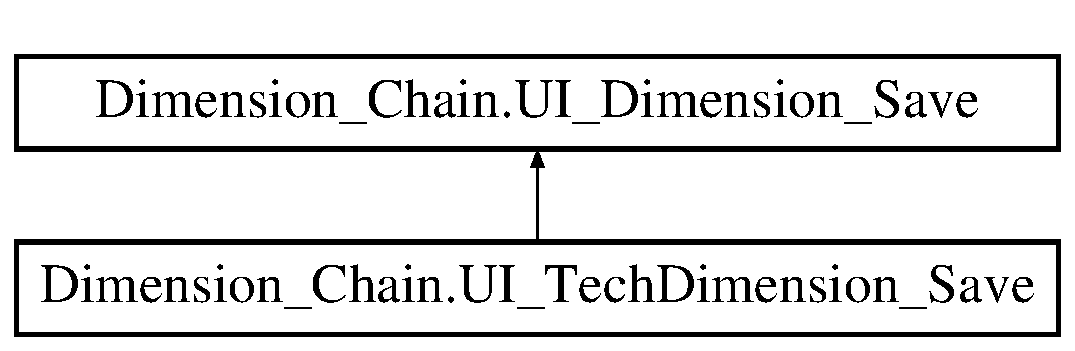
\includegraphics[height=2.000000cm]{class_dimension___chain_1_1_u_i___tech_dimension___save}
\end{center}
\end{figure}
\subsection*{Public Member Functions}
\begin{DoxyCompactItemize}
\item 
\mbox{\hyperlink{class_dimension___chain_1_1_u_i___tech_dimension___save_a3a30dd2f9cd3a59063a4d0203499d5d0}{U\+I\+\_\+\+Tech\+Dimension\+\_\+\+Save}} (\mbox{\hyperlink{class_dimension___chain_1_1_u_i___tech_dimension}{U\+I\+\_\+\+Tech\+Dimension}} dim)
\end{DoxyCompactItemize}
\subsection*{Public Attributes}
\begin{DoxyCompactItemize}
\item 
double \mbox{\hyperlink{class_dimension___chain_1_1_u_i___tech_dimension___save_ac901919246cbc990670d8167fbb74701}{nominal}}
\item 
double \mbox{\hyperlink{class_dimension___chain_1_1_u_i___tech_dimension___save_a772f22894e61f822e2e31981df04b1ed}{up}}
\item 
double \mbox{\hyperlink{class_dimension___chain_1_1_u_i___tech_dimension___save_aa66f7ad4eae6810976b333fdcf4da52c}{down}}
\end{DoxyCompactItemize}


\subsection{Constructor \& Destructor Documentation}
\mbox{\Hypertarget{class_dimension___chain_1_1_u_i___tech_dimension___save_a3a30dd2f9cd3a59063a4d0203499d5d0}\label{class_dimension___chain_1_1_u_i___tech_dimension___save_a3a30dd2f9cd3a59063a4d0203499d5d0}} 
\index{Dimension\+\_\+\+Chain\+::\+U\+I\+\_\+\+Tech\+Dimension\+\_\+\+Save@{Dimension\+\_\+\+Chain\+::\+U\+I\+\_\+\+Tech\+Dimension\+\_\+\+Save}!U\+I\+\_\+\+Tech\+Dimension\+\_\+\+Save@{U\+I\+\_\+\+Tech\+Dimension\+\_\+\+Save}}
\index{U\+I\+\_\+\+Tech\+Dimension\+\_\+\+Save@{U\+I\+\_\+\+Tech\+Dimension\+\_\+\+Save}!Dimension\+\_\+\+Chain\+::\+U\+I\+\_\+\+Tech\+Dimension\+\_\+\+Save@{Dimension\+\_\+\+Chain\+::\+U\+I\+\_\+\+Tech\+Dimension\+\_\+\+Save}}
\subsubsection{\texorpdfstring{U\+I\+\_\+\+Tech\+Dimension\+\_\+\+Save()}{UI\_TechDimension\_Save()}}
{\footnotesize\ttfamily Dimension\+\_\+\+Chain.\+U\+I\+\_\+\+Tech\+Dimension\+\_\+\+Save.\+U\+I\+\_\+\+Tech\+Dimension\+\_\+\+Save (\begin{DoxyParamCaption}\item[{\mbox{\hyperlink{class_dimension___chain_1_1_u_i___tech_dimension}{U\+I\+\_\+\+Tech\+Dimension}}}]{dim }\end{DoxyParamCaption})}



\subsection{Member Data Documentation}
\mbox{\Hypertarget{class_dimension___chain_1_1_u_i___tech_dimension___save_aa66f7ad4eae6810976b333fdcf4da52c}\label{class_dimension___chain_1_1_u_i___tech_dimension___save_aa66f7ad4eae6810976b333fdcf4da52c}} 
\index{Dimension\+\_\+\+Chain\+::\+U\+I\+\_\+\+Tech\+Dimension\+\_\+\+Save@{Dimension\+\_\+\+Chain\+::\+U\+I\+\_\+\+Tech\+Dimension\+\_\+\+Save}!down@{down}}
\index{down@{down}!Dimension\+\_\+\+Chain\+::\+U\+I\+\_\+\+Tech\+Dimension\+\_\+\+Save@{Dimension\+\_\+\+Chain\+::\+U\+I\+\_\+\+Tech\+Dimension\+\_\+\+Save}}
\subsubsection{\texorpdfstring{down}{down}}
{\footnotesize\ttfamily double Dimension\+\_\+\+Chain.\+U\+I\+\_\+\+Tech\+Dimension\+\_\+\+Save.\+down}

\mbox{\Hypertarget{class_dimension___chain_1_1_u_i___tech_dimension___save_ac901919246cbc990670d8167fbb74701}\label{class_dimension___chain_1_1_u_i___tech_dimension___save_ac901919246cbc990670d8167fbb74701}} 
\index{Dimension\+\_\+\+Chain\+::\+U\+I\+\_\+\+Tech\+Dimension\+\_\+\+Save@{Dimension\+\_\+\+Chain\+::\+U\+I\+\_\+\+Tech\+Dimension\+\_\+\+Save}!nominal@{nominal}}
\index{nominal@{nominal}!Dimension\+\_\+\+Chain\+::\+U\+I\+\_\+\+Tech\+Dimension\+\_\+\+Save@{Dimension\+\_\+\+Chain\+::\+U\+I\+\_\+\+Tech\+Dimension\+\_\+\+Save}}
\subsubsection{\texorpdfstring{nominal}{nominal}}
{\footnotesize\ttfamily double Dimension\+\_\+\+Chain.\+U\+I\+\_\+\+Tech\+Dimension\+\_\+\+Save.\+nominal}

\mbox{\Hypertarget{class_dimension___chain_1_1_u_i___tech_dimension___save_a772f22894e61f822e2e31981df04b1ed}\label{class_dimension___chain_1_1_u_i___tech_dimension___save_a772f22894e61f822e2e31981df04b1ed}} 
\index{Dimension\+\_\+\+Chain\+::\+U\+I\+\_\+\+Tech\+Dimension\+\_\+\+Save@{Dimension\+\_\+\+Chain\+::\+U\+I\+\_\+\+Tech\+Dimension\+\_\+\+Save}!up@{up}}
\index{up@{up}!Dimension\+\_\+\+Chain\+::\+U\+I\+\_\+\+Tech\+Dimension\+\_\+\+Save@{Dimension\+\_\+\+Chain\+::\+U\+I\+\_\+\+Tech\+Dimension\+\_\+\+Save}}
\subsubsection{\texorpdfstring{up}{up}}
{\footnotesize\ttfamily double Dimension\+\_\+\+Chain.\+U\+I\+\_\+\+Tech\+Dimension\+\_\+\+Save.\+up}



The documentation for this class was generated from the following file\+:\begin{DoxyCompactItemize}
\item 
\mbox{\hyperlink{_save_8cs}{Save.\+cs}}\end{DoxyCompactItemize}

\hypertarget{class_dimension___chain_1_1_value}{}\section{Dimension\+\_\+\+Chain.\+Value Class Reference}
\label{class_dimension___chain_1_1_value}\index{Dimension\+\_\+\+Chain.\+Value@{Dimension\+\_\+\+Chain.\+Value}}
\subsection*{Public Member Functions}
\begin{DoxyCompactItemize}
\item 
\mbox{\hyperlink{class_dimension___chain_1_1_value_a20ddc0b81f42f4fd162f00340beb093f}{Value}} ()
\item 
\mbox{\hyperlink{class_dimension___chain_1_1_value_adbce27eeb02d593d6baba31ef988f7a8}{Value}} (double \mbox{\hyperlink{class_dimension___chain_1_1_value_ad8021f1acadd25ca6ed51539a54abcff}{nominal}}, double \mbox{\hyperlink{class_dimension___chain_1_1_value_a527768f61f2911e1ccadcb479974c073}{up\+Tolerance}}, double \mbox{\hyperlink{class_dimension___chain_1_1_value_a03fea4a7e636ffccff17ba0dc711d681}{down\+Tolerance}})
\item 
\mbox{\hyperlink{class_dimension___chain_1_1_value}{Value}} \mbox{\hyperlink{class_dimension___chain_1_1_value_a85d60135a70b5e670bf0a1e1cc0967da}{Inverse}} ()
\end{DoxyCompactItemize}
\subsection*{Public Attributes}
\begin{DoxyCompactItemize}
\item 
double \mbox{\hyperlink{class_dimension___chain_1_1_value_ad8021f1acadd25ca6ed51539a54abcff}{nominal}}
\item 
double \mbox{\hyperlink{class_dimension___chain_1_1_value_a527768f61f2911e1ccadcb479974c073}{up\+Tolerance}}
\item 
double \mbox{\hyperlink{class_dimension___chain_1_1_value_a03fea4a7e636ffccff17ba0dc711d681}{down\+Tolerance}}
\item 
bool \mbox{\hyperlink{class_dimension___chain_1_1_value_a6095f62a5449867ec99c705006846734}{error}} = false
\end{DoxyCompactItemize}


\subsection{Constructor \& Destructor Documentation}
\mbox{\Hypertarget{class_dimension___chain_1_1_value_a20ddc0b81f42f4fd162f00340beb093f}\label{class_dimension___chain_1_1_value_a20ddc0b81f42f4fd162f00340beb093f}} 
\index{Dimension\+\_\+\+Chain\+::\+Value@{Dimension\+\_\+\+Chain\+::\+Value}!Value@{Value}}
\index{Value@{Value}!Dimension\+\_\+\+Chain\+::\+Value@{Dimension\+\_\+\+Chain\+::\+Value}}
\subsubsection{\texorpdfstring{Value()}{Value()}\hspace{0.1cm}{\footnotesize\ttfamily [1/2]}}
{\footnotesize\ttfamily Dimension\+\_\+\+Chain.\+Value.\+Value (\begin{DoxyParamCaption}{ }\end{DoxyParamCaption})}

\mbox{\Hypertarget{class_dimension___chain_1_1_value_adbce27eeb02d593d6baba31ef988f7a8}\label{class_dimension___chain_1_1_value_adbce27eeb02d593d6baba31ef988f7a8}} 
\index{Dimension\+\_\+\+Chain\+::\+Value@{Dimension\+\_\+\+Chain\+::\+Value}!Value@{Value}}
\index{Value@{Value}!Dimension\+\_\+\+Chain\+::\+Value@{Dimension\+\_\+\+Chain\+::\+Value}}
\subsubsection{\texorpdfstring{Value()}{Value()}\hspace{0.1cm}{\footnotesize\ttfamily [2/2]}}
{\footnotesize\ttfamily Dimension\+\_\+\+Chain.\+Value.\+Value (\begin{DoxyParamCaption}\item[{double}]{nominal,  }\item[{double}]{up\+Tolerance,  }\item[{double}]{down\+Tolerance }\end{DoxyParamCaption})}



\subsection{Member Function Documentation}
\mbox{\Hypertarget{class_dimension___chain_1_1_value_a85d60135a70b5e670bf0a1e1cc0967da}\label{class_dimension___chain_1_1_value_a85d60135a70b5e670bf0a1e1cc0967da}} 
\index{Dimension\+\_\+\+Chain\+::\+Value@{Dimension\+\_\+\+Chain\+::\+Value}!Inverse@{Inverse}}
\index{Inverse@{Inverse}!Dimension\+\_\+\+Chain\+::\+Value@{Dimension\+\_\+\+Chain\+::\+Value}}
\subsubsection{\texorpdfstring{Inverse()}{Inverse()}}
{\footnotesize\ttfamily \mbox{\hyperlink{class_dimension___chain_1_1_value}{Value}} Dimension\+\_\+\+Chain.\+Value.\+Inverse (\begin{DoxyParamCaption}{ }\end{DoxyParamCaption})}



\subsection{Member Data Documentation}
\mbox{\Hypertarget{class_dimension___chain_1_1_value_a03fea4a7e636ffccff17ba0dc711d681}\label{class_dimension___chain_1_1_value_a03fea4a7e636ffccff17ba0dc711d681}} 
\index{Dimension\+\_\+\+Chain\+::\+Value@{Dimension\+\_\+\+Chain\+::\+Value}!down\+Tolerance@{down\+Tolerance}}
\index{down\+Tolerance@{down\+Tolerance}!Dimension\+\_\+\+Chain\+::\+Value@{Dimension\+\_\+\+Chain\+::\+Value}}
\subsubsection{\texorpdfstring{down\+Tolerance}{downTolerance}}
{\footnotesize\ttfamily double Dimension\+\_\+\+Chain.\+Value.\+down\+Tolerance}

\mbox{\Hypertarget{class_dimension___chain_1_1_value_a6095f62a5449867ec99c705006846734}\label{class_dimension___chain_1_1_value_a6095f62a5449867ec99c705006846734}} 
\index{Dimension\+\_\+\+Chain\+::\+Value@{Dimension\+\_\+\+Chain\+::\+Value}!error@{error}}
\index{error@{error}!Dimension\+\_\+\+Chain\+::\+Value@{Dimension\+\_\+\+Chain\+::\+Value}}
\subsubsection{\texorpdfstring{error}{error}}
{\footnotesize\ttfamily bool Dimension\+\_\+\+Chain.\+Value.\+error = false}

\mbox{\Hypertarget{class_dimension___chain_1_1_value_ad8021f1acadd25ca6ed51539a54abcff}\label{class_dimension___chain_1_1_value_ad8021f1acadd25ca6ed51539a54abcff}} 
\index{Dimension\+\_\+\+Chain\+::\+Value@{Dimension\+\_\+\+Chain\+::\+Value}!nominal@{nominal}}
\index{nominal@{nominal}!Dimension\+\_\+\+Chain\+::\+Value@{Dimension\+\_\+\+Chain\+::\+Value}}
\subsubsection{\texorpdfstring{nominal}{nominal}}
{\footnotesize\ttfamily double Dimension\+\_\+\+Chain.\+Value.\+nominal}

\mbox{\Hypertarget{class_dimension___chain_1_1_value_a527768f61f2911e1ccadcb479974c073}\label{class_dimension___chain_1_1_value_a527768f61f2911e1ccadcb479974c073}} 
\index{Dimension\+\_\+\+Chain\+::\+Value@{Dimension\+\_\+\+Chain\+::\+Value}!up\+Tolerance@{up\+Tolerance}}
\index{up\+Tolerance@{up\+Tolerance}!Dimension\+\_\+\+Chain\+::\+Value@{Dimension\+\_\+\+Chain\+::\+Value}}
\subsubsection{\texorpdfstring{up\+Tolerance}{upTolerance}}
{\footnotesize\ttfamily double Dimension\+\_\+\+Chain.\+Value.\+up\+Tolerance}



The documentation for this class was generated from the following file\+:\begin{DoxyCompactItemize}
\item 
\mbox{\hyperlink{_dimension_8cs}{Dimension.\+cs}}\end{DoxyCompactItemize}

\hypertarget{class_dimension___chain_1_1_vertex}{}\section{Dimension\+\_\+\+Chain.\+Vertex Class Reference}
\label{class_dimension___chain_1_1_vertex}\index{Dimension\+\_\+\+Chain.\+Vertex@{Dimension\+\_\+\+Chain.\+Vertex}}
\subsection*{Public Member Functions}
\begin{DoxyCompactItemize}
\item 
\mbox{\hyperlink{class_dimension___chain_1_1_vertex_a57ae2d0098e07307070c4e140980527c}{Vertex}} (int \mbox{\hyperlink{class_dimension___chain_1_1_vertex_aa803e8c5e381e30ad498686633a3a4ae}{num}})
\item 
void \mbox{\hyperlink{class_dimension___chain_1_1_vertex_a027ea03e13737bce5e7de4fab41c828d}{Add\+Neighbor}} (\mbox{\hyperlink{class_dimension___chain_1_1_vertex}{Vertex}} neighbor, \mbox{\hyperlink{class_dimension___chain_1_1_value}{Value}} val, \mbox{\hyperlink{class_dimension___chain_1_1_dimension}{Dimension}} dim)
\item 
void \mbox{\hyperlink{class_dimension___chain_1_1_vertex_a912f3caec2dfba7f1e3f955ad20d1736}{Delete\+Neighbor}} (\mbox{\hyperlink{class_dimension___chain_1_1_vertex}{Vertex}} neighbor)
\end{DoxyCompactItemize}
\subsection*{Public Attributes}
\begin{DoxyCompactItemize}
\item 
int \mbox{\hyperlink{class_dimension___chain_1_1_vertex_aa803e8c5e381e30ad498686633a3a4ae}{num}}
\item 
List$<$ \mbox{\hyperlink{class_dimension___chain_1_1_vertex}{Vertex}} $>$ \mbox{\hyperlink{class_dimension___chain_1_1_vertex_a88374fb71c7e0c494307b501cf1cd3bd}{neighbors}} = new List$<$\mbox{\hyperlink{class_dimension___chain_1_1_vertex}{Vertex}}$>$()
\item 
bool \mbox{\hyperlink{class_dimension___chain_1_1_vertex_af2e30f955bb2d8cba8f8c4846ecc767d}{visited}} = false
\item 
Dictionary$<$ \mbox{\hyperlink{class_dimension___chain_1_1_vertex}{Vertex}}, \mbox{\hyperlink{class_dimension___chain_1_1_dimension}{Dimension}} $>$ \mbox{\hyperlink{class_dimension___chain_1_1_vertex_af26ff58e451fc5b0777e08a2fb849800}{dimension\+To}} = new Dictionary$<$\mbox{\hyperlink{class_dimension___chain_1_1_vertex}{Vertex}}, \mbox{\hyperlink{class_dimension___chain_1_1_dimension}{Dimension}}$>$()
\item 
Dictionary$<$ \mbox{\hyperlink{class_dimension___chain_1_1_vertex}{Vertex}}, \mbox{\hyperlink{class_dimension___chain_1_1_value}{Value}} $>$ \mbox{\hyperlink{class_dimension___chain_1_1_vertex_a4143488432955c4f229b0329ab8cd6e1}{distance\+To}} = new Dictionary$<$\mbox{\hyperlink{class_dimension___chain_1_1_vertex}{Vertex}}, \mbox{\hyperlink{class_dimension___chain_1_1_value}{Value}}$>$()
\end{DoxyCompactItemize}


\subsection{Constructor \& Destructor Documentation}
\mbox{\Hypertarget{class_dimension___chain_1_1_vertex_a57ae2d0098e07307070c4e140980527c}\label{class_dimension___chain_1_1_vertex_a57ae2d0098e07307070c4e140980527c}} 
\index{Dimension\+\_\+\+Chain\+::\+Vertex@{Dimension\+\_\+\+Chain\+::\+Vertex}!Vertex@{Vertex}}
\index{Vertex@{Vertex}!Dimension\+\_\+\+Chain\+::\+Vertex@{Dimension\+\_\+\+Chain\+::\+Vertex}}
\subsubsection{\texorpdfstring{Vertex()}{Vertex()}}
{\footnotesize\ttfamily Dimension\+\_\+\+Chain.\+Vertex.\+Vertex (\begin{DoxyParamCaption}\item[{int}]{num }\end{DoxyParamCaption})}



\subsection{Member Function Documentation}
\mbox{\Hypertarget{class_dimension___chain_1_1_vertex_a027ea03e13737bce5e7de4fab41c828d}\label{class_dimension___chain_1_1_vertex_a027ea03e13737bce5e7de4fab41c828d}} 
\index{Dimension\+\_\+\+Chain\+::\+Vertex@{Dimension\+\_\+\+Chain\+::\+Vertex}!Add\+Neighbor@{Add\+Neighbor}}
\index{Add\+Neighbor@{Add\+Neighbor}!Dimension\+\_\+\+Chain\+::\+Vertex@{Dimension\+\_\+\+Chain\+::\+Vertex}}
\subsubsection{\texorpdfstring{Add\+Neighbor()}{AddNeighbor()}}
{\footnotesize\ttfamily void Dimension\+\_\+\+Chain.\+Vertex.\+Add\+Neighbor (\begin{DoxyParamCaption}\item[{\mbox{\hyperlink{class_dimension___chain_1_1_vertex}{Vertex}}}]{neighbor,  }\item[{\mbox{\hyperlink{class_dimension___chain_1_1_value}{Value}}}]{val,  }\item[{\mbox{\hyperlink{class_dimension___chain_1_1_dimension}{Dimension}}}]{dim }\end{DoxyParamCaption})}

\mbox{\Hypertarget{class_dimension___chain_1_1_vertex_a912f3caec2dfba7f1e3f955ad20d1736}\label{class_dimension___chain_1_1_vertex_a912f3caec2dfba7f1e3f955ad20d1736}} 
\index{Dimension\+\_\+\+Chain\+::\+Vertex@{Dimension\+\_\+\+Chain\+::\+Vertex}!Delete\+Neighbor@{Delete\+Neighbor}}
\index{Delete\+Neighbor@{Delete\+Neighbor}!Dimension\+\_\+\+Chain\+::\+Vertex@{Dimension\+\_\+\+Chain\+::\+Vertex}}
\subsubsection{\texorpdfstring{Delete\+Neighbor()}{DeleteNeighbor()}}
{\footnotesize\ttfamily void Dimension\+\_\+\+Chain.\+Vertex.\+Delete\+Neighbor (\begin{DoxyParamCaption}\item[{\mbox{\hyperlink{class_dimension___chain_1_1_vertex}{Vertex}}}]{neighbor }\end{DoxyParamCaption})}



\subsection{Member Data Documentation}
\mbox{\Hypertarget{class_dimension___chain_1_1_vertex_af26ff58e451fc5b0777e08a2fb849800}\label{class_dimension___chain_1_1_vertex_af26ff58e451fc5b0777e08a2fb849800}} 
\index{Dimension\+\_\+\+Chain\+::\+Vertex@{Dimension\+\_\+\+Chain\+::\+Vertex}!dimension\+To@{dimension\+To}}
\index{dimension\+To@{dimension\+To}!Dimension\+\_\+\+Chain\+::\+Vertex@{Dimension\+\_\+\+Chain\+::\+Vertex}}
\subsubsection{\texorpdfstring{dimension\+To}{dimensionTo}}
{\footnotesize\ttfamily Dictionary$<$\mbox{\hyperlink{class_dimension___chain_1_1_vertex}{Vertex}}, \mbox{\hyperlink{class_dimension___chain_1_1_dimension}{Dimension}}$>$ Dimension\+\_\+\+Chain.\+Vertex.\+dimension\+To = new Dictionary$<$\mbox{\hyperlink{class_dimension___chain_1_1_vertex}{Vertex}}, \mbox{\hyperlink{class_dimension___chain_1_1_dimension}{Dimension}}$>$()}

\mbox{\Hypertarget{class_dimension___chain_1_1_vertex_a4143488432955c4f229b0329ab8cd6e1}\label{class_dimension___chain_1_1_vertex_a4143488432955c4f229b0329ab8cd6e1}} 
\index{Dimension\+\_\+\+Chain\+::\+Vertex@{Dimension\+\_\+\+Chain\+::\+Vertex}!distance\+To@{distance\+To}}
\index{distance\+To@{distance\+To}!Dimension\+\_\+\+Chain\+::\+Vertex@{Dimension\+\_\+\+Chain\+::\+Vertex}}
\subsubsection{\texorpdfstring{distance\+To}{distanceTo}}
{\footnotesize\ttfamily Dictionary$<$\mbox{\hyperlink{class_dimension___chain_1_1_vertex}{Vertex}}, \mbox{\hyperlink{class_dimension___chain_1_1_value}{Value}}$>$ Dimension\+\_\+\+Chain.\+Vertex.\+distance\+To = new Dictionary$<$\mbox{\hyperlink{class_dimension___chain_1_1_vertex}{Vertex}}, \mbox{\hyperlink{class_dimension___chain_1_1_value}{Value}}$>$()}

\mbox{\Hypertarget{class_dimension___chain_1_1_vertex_a88374fb71c7e0c494307b501cf1cd3bd}\label{class_dimension___chain_1_1_vertex_a88374fb71c7e0c494307b501cf1cd3bd}} 
\index{Dimension\+\_\+\+Chain\+::\+Vertex@{Dimension\+\_\+\+Chain\+::\+Vertex}!neighbors@{neighbors}}
\index{neighbors@{neighbors}!Dimension\+\_\+\+Chain\+::\+Vertex@{Dimension\+\_\+\+Chain\+::\+Vertex}}
\subsubsection{\texorpdfstring{neighbors}{neighbors}}
{\footnotesize\ttfamily List$<$\mbox{\hyperlink{class_dimension___chain_1_1_vertex}{Vertex}}$>$ Dimension\+\_\+\+Chain.\+Vertex.\+neighbors = new List$<$\mbox{\hyperlink{class_dimension___chain_1_1_vertex}{Vertex}}$>$()}

\mbox{\Hypertarget{class_dimension___chain_1_1_vertex_aa803e8c5e381e30ad498686633a3a4ae}\label{class_dimension___chain_1_1_vertex_aa803e8c5e381e30ad498686633a3a4ae}} 
\index{Dimension\+\_\+\+Chain\+::\+Vertex@{Dimension\+\_\+\+Chain\+::\+Vertex}!num@{num}}
\index{num@{num}!Dimension\+\_\+\+Chain\+::\+Vertex@{Dimension\+\_\+\+Chain\+::\+Vertex}}
\subsubsection{\texorpdfstring{num}{num}}
{\footnotesize\ttfamily int Dimension\+\_\+\+Chain.\+Vertex.\+num}

\mbox{\Hypertarget{class_dimension___chain_1_1_vertex_af2e30f955bb2d8cba8f8c4846ecc767d}\label{class_dimension___chain_1_1_vertex_af2e30f955bb2d8cba8f8c4846ecc767d}} 
\index{Dimension\+\_\+\+Chain\+::\+Vertex@{Dimension\+\_\+\+Chain\+::\+Vertex}!visited@{visited}}
\index{visited@{visited}!Dimension\+\_\+\+Chain\+::\+Vertex@{Dimension\+\_\+\+Chain\+::\+Vertex}}
\subsubsection{\texorpdfstring{visited}{visited}}
{\footnotesize\ttfamily bool Dimension\+\_\+\+Chain.\+Vertex.\+visited = false}



The documentation for this class was generated from the following file\+:\begin{DoxyCompactItemize}
\item 
\mbox{\hyperlink{_vertex_8cs}{Vertex.\+cs}}\end{DoxyCompactItemize}

\chapter{File Documentation}
\hypertarget{_app_8xaml_8cs}{}\section{App.\+xaml.\+cs File Reference}
\label{_app_8xaml_8cs}\index{App.\+xaml.\+cs@{App.\+xaml.\+cs}}
\subsection*{Classes}
\begin{DoxyCompactItemize}
\item 
class \mbox{\hyperlink{class_dimension___chain_1_1_app}{Dimension\+\_\+\+Chain.\+App}}
\begin{DoxyCompactList}\small\item\em Логика взаимодействия для App.\+xaml \end{DoxyCompactList}\end{DoxyCompactItemize}
\subsection*{Namespaces}
\begin{DoxyCompactItemize}
\item 
namespace \mbox{\hyperlink{namespace_dimension___chain}{Dimension\+\_\+\+Chain}}
\end{DoxyCompactItemize}

\hypertarget{_constructor_user_control_8xaml_8cs}{}\section{Constructor\+User\+Control.\+xaml.\+cs File Reference}
\label{_constructor_user_control_8xaml_8cs}\index{Constructor\+User\+Control.\+xaml.\+cs@{Constructor\+User\+Control.\+xaml.\+cs}}
\subsection*{Classes}
\begin{DoxyCompactItemize}
\item 
class \mbox{\hyperlink{class_dimension___chain_1_1_constructor_user_control}{Dimension\+\_\+\+Chain.\+Constructor\+User\+Control}}
\begin{DoxyCompactList}\small\item\em Логика взаимодействия для Constructor\+User\+Control.\+xaml \end{DoxyCompactList}\end{DoxyCompactItemize}
\subsection*{Namespaces}
\begin{DoxyCompactItemize}
\item 
namespace \mbox{\hyperlink{namespace_dimension___chain}{Dimension\+\_\+\+Chain}}
\end{DoxyCompactItemize}

\hypertarget{_controller_8cs}{}\section{Controller.\+cs File Reference}
\label{_controller_8cs}\index{Controller.\+cs@{Controller.\+cs}}
\subsection*{Classes}
\begin{DoxyCompactItemize}
\item 
interface \mbox{\hyperlink{interface_dimension___chain_1_1_i_controller}{Dimension\+\_\+\+Chain.\+I\+Controller}}
\item 
class \mbox{\hyperlink{class_dimension___chain_1_1_controller}{Dimension\+\_\+\+Chain.\+Controller}}
\end{DoxyCompactItemize}
\subsection*{Namespaces}
\begin{DoxyCompactItemize}
\item 
namespace \mbox{\hyperlink{namespace_dimension___chain}{Dimension\+\_\+\+Chain}}
\end{DoxyCompactItemize}

\hypertarget{_dimension_8cs}{}\section{Dimension.\+cs File Reference}
\label{_dimension_8cs}\index{Dimension.\+cs@{Dimension.\+cs}}
\subsection*{Classes}
\begin{DoxyCompactItemize}
\item 
class \mbox{\hyperlink{class_dimension___chain_1_1_dimension}{Dimension\+\_\+\+Chain.\+Dimension}}
\item 
class \mbox{\hyperlink{class_dimension___chain_1_1_value}{Dimension\+\_\+\+Chain.\+Value}}
\end{DoxyCompactItemize}
\subsection*{Namespaces}
\begin{DoxyCompactItemize}
\item 
namespace \mbox{\hyperlink{namespace_dimension___chain}{Dimension\+\_\+\+Chain}}
\end{DoxyCompactItemize}
\subsection*{Enumerations}
\begin{DoxyCompactItemize}
\item 
enum \mbox{\hyperlink{namespace_dimension___chain_a6ec9051138598c61cc00acf2547dced4}{Dimension\+\_\+\+Chain.\+type}} \{ \mbox{\hyperlink{namespace_dimension___chain_a6ec9051138598c61cc00acf2547dced4a86476dc11574d5a7c834b43c2b3cb307}{Dimension\+\_\+\+Chain.\+type.\+konstr}}, 
\mbox{\hyperlink{namespace_dimension___chain_a6ec9051138598c61cc00acf2547dced4a7d5fd127b63e3b749194757afe78502e}{Dimension\+\_\+\+Chain.\+type.\+pripusk}}, 
\mbox{\hyperlink{namespace_dimension___chain_a6ec9051138598c61cc00acf2547dced4ad9f9133fb120cd6096870bc2b496805b}{Dimension\+\_\+\+Chain.\+type.\+tech}}, 
\mbox{\hyperlink{namespace_dimension___chain_a6ec9051138598c61cc00acf2547dced4a40a8712b29ac76182ed0c4f632b7d543}{Dimension\+\_\+\+Chain.\+type.\+nul}}
 \}
\end{DoxyCompactItemize}

\hypertarget{_graph_8cs}{}\section{Graph.\+cs File Reference}
\label{_graph_8cs}\index{Graph.\+cs@{Graph.\+cs}}
\subsection*{Classes}
\begin{DoxyCompactItemize}
\item 
class \mbox{\hyperlink{class_dimension___chain_1_1_graph}{Dimension\+\_\+\+Chain.\+Graph}}
\end{DoxyCompactItemize}
\subsection*{Namespaces}
\begin{DoxyCompactItemize}
\item 
namespace \mbox{\hyperlink{namespace_dimension___chain}{Dimension\+\_\+\+Chain}}
\end{DoxyCompactItemize}

\hypertarget{_main_window_8xaml_8cs}{}\section{Main\+Window.\+xaml.\+cs File Reference}
\label{_main_window_8xaml_8cs}\index{Main\+Window.\+xaml.\+cs@{Main\+Window.\+xaml.\+cs}}
\subsection*{Classes}
\begin{DoxyCompactItemize}
\item 
class \mbox{\hyperlink{class_dimension___chain_1_1_main_window}{Dimension\+\_\+\+Chain.\+Main\+Window}}
\begin{DoxyCompactList}\small\item\em Логика взаимодействия для Main\+Window.\+xaml -\/ V\+I\+EW \end{DoxyCompactList}\end{DoxyCompactItemize}
\subsection*{Namespaces}
\begin{DoxyCompactItemize}
\item 
namespace \mbox{\hyperlink{namespace_dimension___chain}{Dimension\+\_\+\+Chain}}
\end{DoxyCompactItemize}

\hypertarget{_mega_vertex_8cs}{}\section{Mega\+Vertex.\+cs File Reference}
\label{_mega_vertex_8cs}\index{Mega\+Vertex.\+cs@{Mega\+Vertex.\+cs}}
\subsection*{Classes}
\begin{DoxyCompactItemize}
\item 
class \mbox{\hyperlink{class_dimension___chain_1_1_mega_vertex}{Dimension\+\_\+\+Chain.\+Mega\+Vertex}}
\end{DoxyCompactItemize}
\subsection*{Namespaces}
\begin{DoxyCompactItemize}
\item 
namespace \mbox{\hyperlink{namespace_dimension___chain}{Dimension\+\_\+\+Chain}}
\end{DoxyCompactItemize}

\hypertarget{_methods_8cs}{}\section{Methods.\+cs File Reference}
\label{_methods_8cs}\index{Methods.\+cs@{Methods.\+cs}}
\subsection*{Classes}
\begin{DoxyCompactItemize}
\item 
class {\bfseries Dimension\+\_\+\+Chain.\+Methods}
\end{DoxyCompactItemize}
\subsection*{Namespaces}
\begin{DoxyCompactItemize}
\item 
namespace \mbox{\hyperlink{namespace_dimension___chain}{Dimension\+\_\+\+Chain}}
\end{DoxyCompactItemize}

\hypertarget{_pripusk_user_control_8xaml_8cs}{}\section{Pripusk\+User\+Control.\+xaml.\+cs File Reference}
\label{_pripusk_user_control_8xaml_8cs}\index{Pripusk\+User\+Control.\+xaml.\+cs@{Pripusk\+User\+Control.\+xaml.\+cs}}
\subsection*{Classes}
\begin{DoxyCompactItemize}
\item 
class \mbox{\hyperlink{class_dimension___chain_1_1_pripusk_user_control}{Dimension\+\_\+\+Chain.\+Pripusk\+User\+Control}}
\begin{DoxyCompactList}\small\item\em Логика взаимодействия для Pripusk\+User\+Control.\+xaml \end{DoxyCompactList}\end{DoxyCompactItemize}
\subsection*{Namespaces}
\begin{DoxyCompactItemize}
\item 
namespace \mbox{\hyperlink{namespace_dimension___chain}{Dimension\+\_\+\+Chain}}
\end{DoxyCompactItemize}

\hypertarget{_save_8cs}{}\section{Save.\+cs File Reference}
\label{_save_8cs}\index{Save.\+cs@{Save.\+cs}}
\subsection*{Classes}
\begin{DoxyCompactItemize}
\item 
class \mbox{\hyperlink{class_dimension___chain_1_1_save}{Dimension\+\_\+\+Chain.\+Save}}
\item 
class \mbox{\hyperlink{class_dimension___chain_1_1_u_i___dimension___save}{Dimension\+\_\+\+Chain.\+U\+I\+\_\+\+Dimension\+\_\+\+Save}}
\item 
class \mbox{\hyperlink{class_dimension___chain_1_1_u_i___tech_dimension___save}{Dimension\+\_\+\+Chain.\+U\+I\+\_\+\+Tech\+Dimension\+\_\+\+Save}}
\item 
class \mbox{\hyperlink{class_dimension___chain_1_1_u_i___constr_dimension___save}{Dimension\+\_\+\+Chain.\+U\+I\+\_\+\+Constr\+Dimension\+\_\+\+Save}}
\item 
class \mbox{\hyperlink{class_dimension___chain_1_1_u_i___pripusk_dimension___save}{Dimension\+\_\+\+Chain.\+U\+I\+\_\+\+Pripusk\+Dimension\+\_\+\+Save}}
\end{DoxyCompactItemize}
\subsection*{Namespaces}
\begin{DoxyCompactItemize}
\item 
namespace \mbox{\hyperlink{namespace_dimension___chain}{Dimension\+\_\+\+Chain}}
\end{DoxyCompactItemize}

\hypertarget{_tech_graph_8cs}{}\section{Tech\+Graph.\+cs File Reference}
\label{_tech_graph_8cs}\index{Tech\+Graph.\+cs@{Tech\+Graph.\+cs}}
\subsection*{Classes}
\begin{DoxyCompactItemize}
\item 
class \mbox{\hyperlink{class_dimension___chain_1_1_tech_graph}{Dimension\+\_\+\+Chain.\+Tech\+Graph}}
\begin{DoxyCompactList}\small\item\em Граф, состоящий из вершин, которые связаны технологическими дугами \end{DoxyCompactList}\end{DoxyCompactItemize}
\subsection*{Namespaces}
\begin{DoxyCompactItemize}
\item 
namespace \mbox{\hyperlink{namespace_dimension___chain}{Dimension\+\_\+\+Chain}}
\end{DoxyCompactItemize}

\hypertarget{_tech_user_control_8xaml_8cs}{}\section{Tech\+User\+Control.\+xaml.\+cs File Reference}
\label{_tech_user_control_8xaml_8cs}\index{Tech\+User\+Control.\+xaml.\+cs@{Tech\+User\+Control.\+xaml.\+cs}}
\subsection*{Classes}
\begin{DoxyCompactItemize}
\item 
class \mbox{\hyperlink{class_dimension___chain_1_1_tech_user_control}{Dimension\+\_\+\+Chain.\+Tech\+User\+Control}}
\begin{DoxyCompactList}\small\item\em Логика взаимодействия для Dimension\+User\+Control.\+xaml \end{DoxyCompactList}\end{DoxyCompactItemize}
\subsection*{Namespaces}
\begin{DoxyCompactItemize}
\item 
namespace \mbox{\hyperlink{namespace_dimension___chain}{Dimension\+\_\+\+Chain}}
\end{DoxyCompactItemize}

\hypertarget{_u_i___constr_dimension_8cs}{}\section{U\+I\+\_\+\+Constr\+Dimension.\+cs File Reference}
\label{_u_i___constr_dimension_8cs}\index{U\+I\+\_\+\+Constr\+Dimension.\+cs@{U\+I\+\_\+\+Constr\+Dimension.\+cs}}
\subsection*{Classes}
\begin{DoxyCompactItemize}
\item 
class \mbox{\hyperlink{class_dimension___chain_1_1_u_i___constr_dimension}{Dimension\+\_\+\+Chain.\+U\+I\+\_\+\+Constr\+Dimension}}
\end{DoxyCompactItemize}
\subsection*{Namespaces}
\begin{DoxyCompactItemize}
\item 
namespace \mbox{\hyperlink{namespace_dimension___chain}{Dimension\+\_\+\+Chain}}
\end{DoxyCompactItemize}

\hypertarget{_u_i___dimension_8cs}{}\section{U\+I\+\_\+\+Dimension.\+cs File Reference}
\label{_u_i___dimension_8cs}\index{U\+I\+\_\+\+Dimension.\+cs@{U\+I\+\_\+\+Dimension.\+cs}}
\subsection*{Classes}
\begin{DoxyCompactItemize}
\item 
class \mbox{\hyperlink{class_dimension___chain_1_1_u_i___dimension}{Dimension\+\_\+\+Chain.\+U\+I\+\_\+\+Dimension}}
\item 
class \mbox{\hyperlink{class_dimension___chain_1_1_native_methods}{Dimension\+\_\+\+Chain.\+Native\+Methods}}
\end{DoxyCompactItemize}
\subsection*{Namespaces}
\begin{DoxyCompactItemize}
\item 
namespace \mbox{\hyperlink{namespace_dimension___chain}{Dimension\+\_\+\+Chain}}
\end{DoxyCompactItemize}

\hypertarget{_u_i___dimension_partial_8cs}{}\section{U\+I\+\_\+\+Dimension\+Partial.\+cs File Reference}
\label{_u_i___dimension_partial_8cs}\index{U\+I\+\_\+\+Dimension\+Partial.\+cs@{U\+I\+\_\+\+Dimension\+Partial.\+cs}}
\subsection*{Classes}
\begin{DoxyCompactItemize}
\item 
class \mbox{\hyperlink{class_dimension___chain_1_1_u_i___dimension}{Dimension\+\_\+\+Chain.\+U\+I\+\_\+\+Dimension}}
\item 
class \mbox{\hyperlink{class_dimension___chain_1_1_u_i___tech_dimension}{Dimension\+\_\+\+Chain.\+U\+I\+\_\+\+Tech\+Dimension}}
\item 
class \mbox{\hyperlink{class_dimension___chain_1_1_u_i___pripusk_dimension}{Dimension\+\_\+\+Chain.\+U\+I\+\_\+\+Pripusk\+Dimension}}
\item 
class \mbox{\hyperlink{class_dimension___chain_1_1_u_i___constr_dimension}{Dimension\+\_\+\+Chain.\+U\+I\+\_\+\+Constr\+Dimension}}
\end{DoxyCompactItemize}
\subsection*{Namespaces}
\begin{DoxyCompactItemize}
\item 
namespace \mbox{\hyperlink{namespace_dimension___chain}{Dimension\+\_\+\+Chain}}
\end{DoxyCompactItemize}

\hypertarget{_u_i___pripusk_dimension_8cs}{}\section{U\+I\+\_\+\+Pripusk\+Dimension.\+cs File Reference}
\label{_u_i___pripusk_dimension_8cs}\index{U\+I\+\_\+\+Pripusk\+Dimension.\+cs@{U\+I\+\_\+\+Pripusk\+Dimension.\+cs}}
\subsection*{Classes}
\begin{DoxyCompactItemize}
\item 
class \mbox{\hyperlink{class_dimension___chain_1_1_u_i___pripusk_dimension}{Dimension\+\_\+\+Chain.\+U\+I\+\_\+\+Pripusk\+Dimension}}
\end{DoxyCompactItemize}
\subsection*{Namespaces}
\begin{DoxyCompactItemize}
\item 
namespace \mbox{\hyperlink{namespace_dimension___chain}{Dimension\+\_\+\+Chain}}
\end{DoxyCompactItemize}

\hypertarget{_u_i___tech_dimension_8cs}{}\section{U\+I\+\_\+\+Tech\+Dimension.\+cs File Reference}
\label{_u_i___tech_dimension_8cs}\index{U\+I\+\_\+\+Tech\+Dimension.\+cs@{U\+I\+\_\+\+Tech\+Dimension.\+cs}}
\subsection*{Classes}
\begin{DoxyCompactItemize}
\item 
class \mbox{\hyperlink{class_dimension___chain_1_1_u_i___tech_dimension}{Dimension\+\_\+\+Chain.\+U\+I\+\_\+\+Tech\+Dimension}}
\end{DoxyCompactItemize}
\subsection*{Namespaces}
\begin{DoxyCompactItemize}
\item 
namespace \mbox{\hyperlink{namespace_dimension___chain}{Dimension\+\_\+\+Chain}}
\end{DoxyCompactItemize}

\hypertarget{_vertex_8cs}{}\section{Vertex.\+cs File Reference}
\label{_vertex_8cs}\index{Vertex.\+cs@{Vertex.\+cs}}
\subsection*{Classes}
\begin{DoxyCompactItemize}
\item 
class \mbox{\hyperlink{class_dimension___chain_1_1_vertex}{Dimension\+\_\+\+Chain.\+Vertex}}
\end{DoxyCompactItemize}
\subsection*{Namespaces}
\begin{DoxyCompactItemize}
\item 
namespace \mbox{\hyperlink{namespace_dimension___chain}{Dimension\+\_\+\+Chain}}
\end{DoxyCompactItemize}
\subsection*{Macros}
\begin{DoxyCompactItemize}
\item 
\#define \mbox{\hyperlink{_vertex_8cs_ae285311ed52dd83bff9d175ded67efb3}{d2}}
\end{DoxyCompactItemize}


\subsection{Macro Definition Documentation}
\mbox{\Hypertarget{_vertex_8cs_ae285311ed52dd83bff9d175ded67efb3}\label{_vertex_8cs_ae285311ed52dd83bff9d175ded67efb3}} 
\index{Vertex.\+cs@{Vertex.\+cs}!d2@{d2}}
\index{d2@{d2}!Vertex.\+cs@{Vertex.\+cs}}
\subsubsection{\texorpdfstring{d2}{d2}}
{\footnotesize\ttfamily \#define d2}


%--- End generated contents ---

% Index
\backmatter
\newpage
\phantomsection
\clearemptydoublepage
\addcontentsline{toc}{chapter}{Index}
\printindex

\end{document}
